
%-----------------------------------------------------------------------------------------------------  
%	INCLUSIÓN DE PAQUETES BÁSICOS.
%-----------------------------------------------------------------------------------------------------

\documentclass[11pt, a4paper,twoside]{article}
\usepackage{enumerate}
\usepackage{wrapfig}
\usepackage{graphicx}
\usepackage{tikz,pgfplots}
\pgfplotsset{compat=1.15}
\usepackage{mathrsfs}
\usetikzlibrary{arrows}
\usepackage{wrapfig}
\usepackage{cutwin}
\usetikzlibrary{quotes,angles}
\usepackage{changepage}
\usetikzlibrary{decorations.pathmorphing}
\usepackage[bottom]{footmisc}
\usepackage{imakeidx}

% Comando para índice final de términos, que enfatice conceptos y los añada al indice final.

\newcommand{\iindex}[1]{\emph{#1}\index{#1}} 

%-----------------------------------------------------------------------------------------------------
%	SELECCIÓN DEL LENGUAJE
%-----------------------------------------------------------------------------------------------------

% Paquetes para adaptar Látex al Español:
\usepackage[spanish,es-noquoting, es-tabla, es-lcroman,galician]{babel} % Cambia
\usepackage[utf8]{inputenc}                                    % Permite los acentos.
\selectlanguage{galician}                                       % Selecciono como lenguaje el Español.


%-----------------------------------------------------------------------------------------------------
%	SELECCIÓN DE LA FUENTE
%-----------------------------------------------------------------------------------------------------

% Fuente utilizada.
\usepackage{courier}                    % Fuente Courier.
\usepackage{microtype}                  % Mejora la letra final de cara al lector.

%-----------------------------------------------------------------------------------------------------
%	ESTILO DE PÁGINA
%-----------------------------------------------------------------------------------------------------

% Paquetes para el diseño de página:
\usepackage{fancyhdr}               % Utilizado para hacer títulos propios.
\usepackage{lastpage}               % Referencia a la última página. Utilizado para el pie de página.
\usepackage{extramarks}             % Marcas extras. Utilizado en pie de página y cabecera.
\usepackage[parfill]{parskip}       % Crea una nueva línea entre párrafos.
\usepackage{geometry}               % Asigna la "geometría" de las páginas.

% Se elige el estilo fancy y márgenes de 2 centímetros.

\geometry{left=2cm,right=2cm,top=2cm,bottom=2cm,headheight=1cm,headsep=0.5cm} % Márgenes y cabecera.
% Se limpia la cabecera y el pie de página para poder rehacerlos luego.
\pagestyle{fancy} %Importante que esté despues de \geometry
\fancyhf{}

% Espacios en el documento:
\linespread{1.1}                        % Espacio entre líneas.
\setlength\parindent{0pt}               % Selecciona la indentación para cada inicio de párrafo.

% Cabecera del documento. Se ajusta la línea de la cabecera.
\renewcommand\headrule{
	\begin{minipage}{1\textwidth}
		\hrule width \hsize
	\end{minipage}
}

% Texto de la cabecera:
\lhead{\docauthor}                          % Parte izquierda.
\chead{}                                    % Centro.
\rhead{IEDO}              % Parte derecha.

% Pie de página del documento. Se ajusta la línea del pie de página.
\renewcommand\footrule{
	\begin{minipage}{1\textwidth}
		\hrule width \hsize
	\end{minipage}\par
}

\lfoot{}                                                 % Parte izquierda.
\cfoot{}                                                 % Centro.
\rfoot{Página\ \thepage\ de\ \protect\pageref{LastPage}} % Parte derecha.

%----------------------------------------------------------------------------------------
%	MATEMÁTICAS
%----------------------------------------------------------------------------------------

% Paquetes para matemáticas:
\usepackage{amsmath, amsthm, amssymb, amsfonts, amscd} % Teoremas, fuentes y símbolos.
\usepackage[all]{xy} % Diagramas conmutativos

% Nuevo estilo para definiciones
\newtheoremstyle{definition-style} % Nombre del estilo
{5pt}                % Espacio por encima
{5pt}                % Espacio por debajo
{}                   % Fuente del cuerpo
{}                   % Identación: vacío= sin identación, \parindent = identación del parráfo
{\bf}                % Fuente para la cabecera
{.}                  % Puntuación tras la cabecera
{.5em}               % Espacio tras la cabecera: { } = espacio usal entre palabras, \newline = nueva línea
{}                   % Especificación de la cabecera (si se deja vaía implica 'normal')

% Nuevo estilo para teoremas
\newtheoremstyle{theorem-style} % Nombre del estilo
{5pt}                % Espacio por encima
{5pt}                % Espacio por debajo
{\itshape}           % Fuente del cuerpo
{}                   % Identación: vacío= sin identación, \parindent = identación del parráfo
{\bf}                % Fuente para la cabecera
{.}                  % Puntuación tras la cabecera
{.5em}               % Espacio tras la cabecera: { } = espacio usal entre palabras, \newline = nueva línea
{}                   % Especificación de la cabecera (si se deja vaía implica 'normal')

% Nuevo estilo para ejemplos y ejercicios
\newtheoremstyle{example-style} % Nombre del estilo
{5pt}                % Espacio por encima
{5pt}                % Espacio por debajo
{}                   % Fuente del cuerpo
{}                   % Identación: vacío= sin identación, \parindent = identación del parráfo
{\scshape}           % Fuente para la cabecera
{:}                  % Puntuación tras la cabecera
{.5em}               % Espacio tras la cabecera: { } = espacio usal entre palabras, \newline = nueva línea
{}                   % Especificación de la cabecera (si se deja vaía implica 'normal')

% Teoremas:
\theoremstyle{theorem-style}  % Otras posibilidades: plain (por defecto), definition, remark
\newtheorem{theorem}{Teorema}[section]  % [section] indica que el contador se reinicia cada sección
\newtheorem{corollary}[theorem]{Corolario} % [theorem] indica que comparte el contador con theorem
\newtheorem{lemma}[theorem]{Lema}
\newtheorem{proposition}[theorem]{Proposición}
\newtheorem*{question}{Cuestión} % * indica que no tiene contador

%Hacemos que las demostraciones estén identadas
\makeatletter
\renewenvironment{proof}[1][\proofname]{\par
	\pushQED{\qed}%
	\normalfont \topsep6\p@\@plus6\p@\relax
	\list{}{%
		\settowidth{\leftmargin}{\quad:\hskip\labelsep}%
		\setlength{\labelwidth}{0pt}%
		\setlength{\itemindent}{-\leftmargin}%
	}%
	\item[\hskip\labelsep\itshape#1\@addpunct{:}]\ignorespaces
}{%
	\popQED\endlist\@endpefalse
}
\makeatother



% Definiciones, notas, conjeturas
\theoremstyle{definition-style}
\newtheorem{definition}{Definición}[section]
\newtheorem{conjecture}{Conxetura}[section]
\newtheorem*{note}{Nota} % * indica que no tiene contador
\newtheorem*{observation}{Observación} % * indica que no tiene contador
\newtheorem*{properties}{Propiedades}
\newtheorem*{comment}{Comentario}

% Ejemplos, ejercicios
\theoremstyle{example-style}
\newtheorem{example}{Exemplo}[section]
\newtheorem{exercise}{Exercicio}[section]

%Operadores de matematicas

\providecommand{\norm}[1]{\left\lVert#1\right\rVert} % Norma que se adapta a la altura de lo de dentro
\providecommand{\abs}[1]{\left\lvert#1\right\rvert} % Valor absoluto que se adapta a la altura de lo de dentro

%Flechas de inyectividad y sobreyectividad. Notación no estándar.
\def\flechaSobreyectiva{\mathrel{\mkern16mu  \vcenter{\hbox{$\scriptscriptstyle+$}}%
		\mkern-25mu{\longrightarrow}}}
\def\flechaInyectiva{\mathrel{\mkern0mu  \vcenter{\hbox{$\scriptscriptstyle+$}}%
		\mkern-9mu{\longrightarrow}}}
\def\flechaBiyectiva{\mathrel{\mkern16mu  \vcenter{\hbox{$\scriptscriptstyle+$}}\mkern-25mu{\mathrel{\mkern0mu\vcenter{\hbox{$\scriptscriptstyle+$}}\mkern-9mu{\longrightarrow}}}}}
\def\xFlechaInyectiva #1{\mathrel{\ooalign{\thinspace\thinspace$\mapstochar\mkern5mu$\hfil\cr$\xrightarrow{#1}$\cr}}}
\def\xFlechaSobreyectiva #1{\mathrel{\ooalign{\hfil$\mapstochar\mkern5mu$\thinspace\thinspace\cr$\xrightarrow{#1}$\cr}}}

%Llave a la derecha de los elementos, para expresar cascadas lógicas condensando varias lineas en una conclusión. Reciproco a \cases
\newenvironment{rcases}
{\left.\begin{aligned}}
	{\end{aligned}\right\rbrace}

%Apilado de varias lineas en pruebas logicas, sin llaves
\newenvironment{bcases}
{\left.\begin{aligned}}
	{\end{aligned}\right.}

%-----------------------------------------------------------------------------------------------------
%	PORTADA
%-----------------------------------------------------------------------------------------------------

% Formato del titulo. Archivo portada.sty asociado es necesario en el mismo directorio.
\usepackage{portada}


%-----------------------------------------------------------------------------------------------------
%	TÍTULO, AUTOR Y OTROS DATOS DEL DOCUMENTO
%-----------------------------------------------------------------------------------------------------

% Título del documento.
\newcommand{\doctitle}{}
% Subtítulo.
\newcommand{\docsubtitle}{}
% Fecha.
\newcommand{\docdate}{6 \ de \ Xuño \ de \ 2019}
% Asignatura.
\newcommand{\subject}{Introducción ás Ecuacións Diferenciais Ordinarias}
% Autor.
\newcommand{\docauthor}{Manuel de Prada, Jorge Vázquez}
\newcommand{\docaddress}{USC}
\newcommand{\docemail}{manuel.deprada@rai.usc.es\\jorge.vazquez.perez@rai.usc.es}

%-----------------------------------------------------------------------------------------------------
%	RESUMEN
%-------------------------------					----------------------------------------------------------------------

% Resumen del documento. Va en la portada.
% Puedes también dejarlo vacío, en cuyo caso no aparece en la portada.
%\newcommand{\docabstract}{}
\newcommand{\docabstract}{Apuntamentos de parte da materia Introdución ás Ecuacións Diferenciais Ordinarias impartida por Óscar Otero Zarraquiños e Daniel Cao Labora.}


%% Indice con enlaces interactivos en el PDF

\usepackage{hyperref}
\hypersetup{
	colorlinks,
	citecolor=black,
	filecolor=black,
	linkcolor=black,
	urlcolor=black
}
\makeindex[columns=1,  intoc]

%%Diseño de impresión: las secciones empiezan en paginas impares.
\let\oldsection\section
\def\section{\cleardoublepage\oldsection}

\begin{document}

\maketitle

%-----------------------------------------------------------------------------------------------------
%	ÍNDICE
%-----------------------------------------------------------------------------------------------------

% Profundidad del Índice:
%\setcounter{tocdepth}{1}

\newpage
\tableofcontents
\newpage

\section{Tema 1.}

\subsection{Motivacións, xeneralidades e exemplos de ecuacións diferenciais ordinarias.}
\begin{example}
	Un tren viaxa a 90 km/h. Ás 10:00 está no quilómetro 22. Onde está ás 12:30?
\end{example}
\begin{proof}[Solución]
	Tomando $x(t)$ como a posición no instante $t$, sabemos que $ x'(t)=90 $, polo que $ x(t)=90t+k $. Ademais, $ x(10)=22 $, polo que coa ecuación anterior, $ k=-878 $. 
	
	É dicir, $ x(t)=90t-878 $ e en particular $ x(12,5)= 247 $.
\end{proof}

\begin{example}
	Un tren está parado nunha cidade A e avanza cunha velocidade $ v(t)=2170t+20t^3 $ en m/min ata que chega á velocidade de cruceiro, que é de 4500 m/min. Pídese achar:
	\begin{enumerate}[\qquad a)]
		\item Distancia percorrida en 1 minuto.
		\item Tempo que tarda en alcanzar a velocidade de cruceiro.
		\item Metros percorridos cando se alcanza a velocidade de cruceiro.
		\item Quilómetros percorridos en 30 minutos.
		\item Hora á que pasará pola cidade B, situada a 243 km de distancia, saíndo ás 7:00.
	\end{enumerate}
\end{example}
\begin{proof}[Solución] \ 
	\begin{enumerate}[\qquad a)]
	\item[b)] Sexa $x(t)$ a posición no instante $t$. Tomando $v(t)=x'(t)=2170t+20t^3=4500$, despexando resulta $ t=2 $. 
	
	\item Buscamos $ x(1) $, para o que primeiros obteremos a expresión xeral $ x(t) $ que cumpra a condición $ x'(t)=2170t+20t^3 $.
	
	A primitiva desta expresión é $ x(t)=\frac{2170t^2}{2}+\frac{20t^4}{4}+k $. Como $ x(0)=0 $, $ k=0 $ e $ x(1)=1090 $.
	
	\item[c)] Trivial a partir dos apartados a) e b). $ x(2)=4420 $m.
	
	\item[d)] Nos dous primeiros minutos, ata alcanzar a velocidade de cruceiro xa habemos visto que se percorren 4420m. Para os 28 restantes, a velocidade é constante polo que expomos a ecuación $ x'(t)=4500 $. 
	
	Por tanto, $ x(t)=4500t+k $. Sabendo que $ x(2)=4420 $, resulta $ k=-4580 $ e $ x(t)=4500t-4580 $ para $ t>2 $. En particular, $ x(30)=130420 $m $ =130,420 $km.
	
	\item[e)] Sabemos polo apartado anterior que se alcanza o punto D (130420m) aos 30 minutos. Os 112,58 metros restantes percórrense en $ \frac{112,58}{4,5\text{m/min}}\simeq 25 $ minutos, polo que o traxecto en total require de 55 minutos e a hora de chegada é as 7:55. 
	
	Outra maneira rápida é despexar $ t $ na ecuación $ x(t)= 243000=4500t-4580 $.
	\end{enumerate}
\end{proof}
\begin{example}
	$ x(t) $ é a cantidade de medicamento presente no organismo nun instante $ t $. A cantidade diminúe proporcionalmente á cantidade de produto presente no organismo. En $ t_0 $, tomamos 500mg. En 1 hora, a cantidade de medicamento no organismo é de 380mg.
	\begin{enumerate}[\qquad a)]
		\item ¿Que cantidade quedará no corpo en 6h?
		\item ¿Cada canto tempo hai que tomar o medicamento para que haxa entre 100mg e 700mg no organismo? 
	\end{enumerate}
\end{example}
\begin{proof}[Solución] \ 
	\begin{enumerate}[\qquad a)]
		\item Como a cantidade diminúe proporcionalmente á cantidade de medicamento no corpo, temos que se $ x(t) $ é a cantidade de medicamento nun instante $ t $, $ x'(t)=-kx(t) $. Ademais sabemos que $ x(0)=500 $ e $ x(1)=380 $. Para obter a expresión correspondente, razoamos:

		Se $ x'(t)=x(t) $, a única opción é que se trate da exponencial. A nosa expresión é parecida, tratemos de cumprir a igualdade $ x'(t)=-kx(t) $. Observamos que se cumpre para $ x(t)=e^{-kt} $. Agora fixámonos no primeiro punto,  $ x(0)=500 $. Con  $ x(t)=500e^{-kt} $ cumprimos esa condición. Por último, quédanos achar unha $ k $ que cumpra $ x(1)=500e^{-k}=380 $. 
		
		Quédanos $ k=-\log(\frac{38}{50}) $ e por tanto $ x(t)=500e^{\log(\frac{38}{50})t} =500(\frac{19}{25})^t$. En consecuencia, $ x(6)=96,35 $mg.

		\item Queremos obter o $ t $ que cumpra $ 100<x(t)<200 $, para que a dose non baixe do 100mg prescritos e ao tomar de novo a dose de 500mg non supere o 700mg.

		$ x(t)=500(\frac{19}{25})^t$ é unha exponencial decrecente en todo o seu dominio, $ (0, +\infty) $. Despexando $ x(t)=500(\frac{19}{25})^t=100$ obtemos $ t=\log_{\frac{19}{25}}(\frac{1}{5})=5,86 $ e para $ x(t)=200 $, $ t=3,33 $. Por tanto, para manter o medicamento entre o 100mg e 700mg debe renovarse a dose pasada entre 3,33 e 5,86 horas.
	\end{enumerate}
\end{proof}

\subsection{Concepto de EDO e solución.}
\begin{definition}
	Sexa $f: A \subset \mathbb{R} \times \mathbb{R}^n \longrightarrow \mathbb{R}^n$ con $f(t, x)$ unha aplicación. Chamamos \iindex{Ecuación Diferencial Ordinaria} (EDO) de primeira orde dada en forma normal relativa á función $f$ a: 
	\[ x' = f(t, x) \]
	Dise que é de primeira orde porque soamente aparece a primeira derivada e en forma normal xa que $x'$ está despexada (se non sería en forma implícita, é dicir, $h(t, x, x')=0$).
\end{definition}

\begin{definition}
	Dada $\varphi: t \in I \subseteq \mathbb{R} \longrightarrow \varphi (t) \in \mathbb{R}^n$ dicimos que $\varphi$ é \iindex{solución} de $x'=f(t, x)$ se verifica:
	\begin{enumerate}[\quad i)]
		\item $(t, \varphi (t)) \in A$, $\forall t \in I$.
		\item Existe $ \varphi' (t)$, $\forall t \in I$.
		\item $\varphi'(t)=f(t, \varphi(t))$,  $\forall t \in I$.
	\end{enumerate}
	Se $I$ contén a un dos seus extremos entenderemos no punto $2$ que exista a súa derivada lateral.
\end{definition}
\begin{observation}
	Temos que $\varphi: t \in \mathbb{R} \longrightarrow \mathbb{R}^n$ con $\varphi (t) = (\varphi_1 (t), ..., \varphi_n (t))$. Por tanto, que $\varphi' (t) = f(t, \varphi (t))$ significa o seguinte:
	\[\varphi' (t) = (\varphi_1' (t), ..., \varphi_n' (t))\] 
	\[f(t, (x_1, ..., x_n)) = (f_1(t, (x_1, ..., x_n)), ..., f_n(t, (x_1, ..., x_n))) \]
	\[
	M=
	\left({\begin{array}{cc}
		\varphi_1' (t) \\
		\vdots \\
		\varphi_n' (t)
		\end{array} } \right)
	=
	\left({\begin{array}{cc}
		f_1(t, \varphi_1 (t), ..., \varphi_n (t)) \\
		\vdots \\
		f_n(t, \varphi_1 (t), ..., \varphi_n (t))
		\end{array} } \right)
	\]
	É dicir:
	\[\left . {\begin{array}{cc}
		\varphi_1' (t) = f_1(t, \varphi_1 (t), ..., \varphi_n (t)) \\
		\vdots \\
		\varphi_n' (t) = f_n(t, \varphi_1 (t), ..., \varphi_n (t))
		\end{array} } \right. \]
\end{observation}
\subsubsection{Continuidade e clase da solución dunha EDO.}
\begin{definition}
	Dicimos que $ f:A\longrightarrow B $ é de clase $ r $, e escribimos $ f\in C^r(A) $ se as súas derivadas parciais de orde $ r $ son continuas.
\end{definition}
\begin{proposition}
	Se $f$ é continua en $A$, entón $\varphi$ é de clase $C^1$ en $I$.
\end{proposition}
\begin{proof} \ \\
	Por definición de solución $\varphi' (t) = f(t, \varphi (t))$, $t \in I$. Compoñendo da seguinte forma
	\[t \stackrel{g}{\longrightarrow} (t, \varphi (t)) \stackrel{f}{\longrightarrow} f(t, \varphi (t))\]
	temos que, tal e como está definida, $g$ é unha función continua por estar composta de $id$, que é a identidade, e de $\varphi$, que é continua por ser derivable en todos os seus puntos. Ademais, como $f$ é continua por definición e temos que $\varphi' (t) = f(t, \varphi (t))$, $\varphi'$ é continua por composición de continuas.
\end{proof}
\begin{theorem}
	Se $f \in C^r$, $r \in \mathbb{N}$ e $r \geq 1$, entón $\varphi \in C^{r+1}(I)$.
\end{theorem}
\begin{proof}\ \\
	Realizaremos a proba empregando indución. En primeiro lugar probarémolo para $r=1$, é dicir, vexamos que:
	\[f\in C^1(A) \Rightarrow \varphi \in C^2(I).\]
	Como $\varphi' (t) = f(t, \varphi (t))$, como vimos antes temos que:
		\[t \stackrel{g}{\longrightarrow} (t, \varphi (t)) \stackrel{f}{\longrightarrow} f(t, \varphi (t)),\]
	pero, temos que $f \in C^1(A)$ polo que $f$ é continua e pola proposición anterior temos que $\varphi \in C^1$. Por tanto, a composición anterior cumpre que é de clase $C^1$, polo que concluímos que $\varphi \in C^2$. \\
	Supoñamos agora certo para un $r$ arbitrario e probémoslo para $r+1$. Sexa $f \in C^{r+1} (A)$ (polo que $f \in C^r \stackrel{\text{hip.}}{\Rightarrow}$ $\varphi \in C^{r+1}$). Vexamos que $\varphi \in C^{r+2}$.
	\[t \longrightarrow (t, \varphi (t)) \longrightarrow f(t, \varphi (t)) = \varphi' (t).\]
	Neste caso, polo mesmo razoamento que no caso $r=1$ temos que a composición é de clase $C^{r+1}$ por composición de funcións de clase $C^{r+1}$. Por tanto existe $\varphi^{r+2)}$ e é continua, polo que $\varphi \in C^{r+2}$. 
\end{proof}
\subsubsection{Problema do valor inicial.}
Co seguinte exemplo introducimos a problemática de elixir correctamente o intervalo de definición da solución, entre os candidatos. Serviranos para introducir a seguinte sección.
\begin{example}
	Sexa $x' = x^2$, é dicir, $f: (t, x) \in \mathbb{R} \times \mathbb{R} \longrightarrow f(t,x) = x^2 \in \mathbb{R}$. Comprobar que $x(t) = \frac{-1}{t+c}$, $c \in \mathbb{R}$, é solución. Estudar en $ t=1 $.
\end{example}
\begin{proof}[Solución]\ \\
	En primeiro lugar temos que ver que $x'(t) = (x(t))^2 = f(t, x(t))$.
	\[x'(t) = \frac{1}{(t+c)^2} \Rightarrow x'(t) = (\frac{-1}{t+c})^2\]
	Ademais, desta solución sabemos que:
	\[\left. {\begin{array}{cc}
		\lim\limits_{t \to (-c)^{-}} x(t) = \lim\limits_{t \to (-c)^{-}} \frac{-1}{t+c} = +\infty\\
		\lim\limits_{t \to (-c)^{+}} x(t) = \lim\limits_{t \to (-c)^{+}} \frac{-1}{t+c} = -\infty
		\end{array}} \right . \]
	polo que a función ten unha asíntota vertical en $t = -c$. Tamén sabemos que:
	\[\left. {\begin{array}{cc}
		\lim\limits_{t \to +\infty} x(t) = \lim\limits_{t \to +\infty} \frac{-1}{t+c} = 0^-\\
		\lim\limits_{t \to -\infty} x(t) = \lim\limits_{t \to -+\infty} \frac{-1}{t+c} = 0^+
		\end{array}} \right .\]
	polo que temos unha asíntota horizontal en $x = 0$. 
	
	
	\begin{figure}[h]
		\centering
		\begin{tikzpicture}[line cap=round,line join=round,>=triangle 45,x=1cm,y=1cm,scale=0.7]
		\begin{axis}[
		x=1cm,y=1cm,
		axis lines=middle,
		xmin=-2.2696161464380893,
		xmax=5.5453285056459745,
		ymin=-3.5608451100207597,
		ymax=3.87288272976652,
		xtick={-2,-1,...,5},
		ytick={-3,-2,...,3},]
		\clip(-2.2696161464380893,-3.5608451100207597) rectangle (5.5453285056459745,3.87288272976652);
		\draw[line width=1pt,smooth,samples=100,domain=-2.2696161464380893:5.5453285056459745] plot(\x,{0-1/((\x)-4/3)});
		
		\draw (1.371004410996194,0.7087831877032161) node[anchor=north west] {x=4/3};
		\end{axis}
		\end{tikzpicture}
		\caption{Solución do exemplo para $ c=-4/3 $.} \label{E1}
	\end{figure}
	
	

	
	
	Neste caso $A = \mathbb{R} \times \mathbb{R} = \mathbb{R}^2$. Ademais,
	\[\psi:t \in (- \infty, - c) \longrightarrow \psi(t) = \frac{-1}{t+c}\]
	\begin{enumerate}
		\item $(t, \psi(t)) \in A$
		\item $\exists \psi' (t) \ \forall t \in I$
		\item $\psi (t) = f(t, \psi (t))$
	\end{enumerate}
	Por tanto, $\psi$ é unha solución de $x'=x^2$. Ademais,
	\[\varphi:t \in (-c, +\infty ) \longrightarrow \varphi(t) = \frac{-1}{t+c}\]
	tamén é solución pola mesma razón que $\psi$, mentres que:
	\[t \in (- \infty, - c) \cup (-c, +\infty ) \longrightarrow f(t) = \frac{-1}{t+c}\]
	non é solución xa que non está definida nun intervalo. \\
	Ademais, se queremos calcular a solución de $x'=x^2$ que en $t =1$ valla $3$ temos que:
	\[3 = x(1) = \frac{-1}{1+c} \Rightarrow 3 + 3c = -1 \Rightarrow c = -\frac{4}{3}\]
	Por tanto, $x(t) = \frac{-1}{t-\frac{4}{3}}$ verifica que $x'(t) = (x(t))^2$, pasando por $ t=1 $. Ademais, polo visto anteriormente, $\psi$ e $\varphi$ son solucións nos seus respectivos intervalos se facemos que $c = - \frac{4}{3}$. Con todo, neste caso, só $ \psi $ está definida en $ t=1 $.
\end{proof}
\subsection{Problema de Cauchy.}

\begin{definition}
	Dada $x' = f(t, x)$ con $f: A \subset \mathbb{R} \times \mathbb{R}^n \longrightarrow \mathbb{R}^n$ e un punto $(t_0, x_0) \in A$, o problema de Cauchy consiste en buscar unha función:
	\[\varphi : I \subset \mathbb{R} \longrightarrow \mathbb{R}^n\]
	con $I$ un intervalo, que sexa solución de $x' = f(t, x)$ tal que $\varphi (t_0) = x_0$.
\end{definition}

\begin{observation}
¿Unha circunferencia pode ser solución dunha EDO?
\end{observation}
\[ t^2+x^2=c \]
\begin{wrapfigure}{l}{3.5cm}   
	\begin{tikzpicture}[cap=round,>=latex,every node/.style={scale=0.5}]
	\draw[thick] (0cm,0cm) circle(1cm);
	\node[circle,draw=white, fill=white, inner sep=0pt,minimum size=5pt] (b) at (1cm,0) {};
	\node[circle,draw=white, fill=white, inner sep=0pt,minimum size=5pt] (b) at (-1cm,0) {};
	\draw[->] (-1.5cm,0cm) -- (1.5cm,0cm) node[right,fill=white]{$t$};
	\draw[->] (0cm,-1.5cm) -- (0cm,1.5cm) node[above,fill=white]{};
	\node[above left] at (-1cm,0) {$(-\sqrt{c},0)$};
	\node[above right] at (1cm,0) {$(\sqrt{c},0)$};
	\node[above right] at (0.7cm,0.7cm) {$x_1(t)$};
	\node[below right] at (0.7cm,-0.7cm) {$x_2(t)$};
	\end{tikzpicture}
\end{wrapfigure}
Non, xa que non é unha función. Con todo, se tomamos $ x_1=\sqrt{c-t^2} $ e $ x_2=-\sqrt{c-t^2} $, son solución da ecuación $ xx'+t=0 $.

Vexámolo para $ x_1 $.
\[ (c-t^2)^{\frac{1}{2}}\frac{1}{2} (c-t^2)^{-\frac{1}{2}}(-2t)+t=-t+t=0 \]
O seu intervalo de definición será $ c-t^2\geq 0 \Rightarrow t \in [-\sqrt{c}, \sqrt{c}], c>0 $ e é derivable en $ (-\sqrt{c}, \sqrt{c}) $.

A solución escollida será unha ou outra en función da condición inicial.
\[ t\in (-\sqrt{c}, \sqrt{c}) \longrightarrow \begin{cases}
x_1(t)=\sqrt{c-t^2}\\
x_2(t)=-\sqrt{c-t^2}
\end{cases}  \]


\section{Tema 2.}

\begin{definition}
	Sexa $ \varphi:t\in I \subset \mathbb{R}\longrightarrow \mathbb{R}^n $, con $ I $ intervalo, solución da ecuación diferencial definida por $ f:(t,x) \in A \subset \mathbb{R}\times \mathbb{R}^n\longrightarrow f(t,x)\in \mathbb{R}^n$, tal que $ x'=f(t,x) $.
\end{definition}

Chamamos \iindex{traxectoria} de $ \varphi $ ao conxunto:
\[  \tau (\varphi)=\{ (t, \varphi(t)), t\in I\} \]
Se $ \varphi(t_0)=x_0 $, chamaremos \iindex{semitraxectoria positiva} de $ \varphi $ ao conxunto:
\[ \tau^+ (\varphi)=\{ (t, \varphi(t)) : t\in I, t>t_0\}  \]
Analogamente, a \iindex{semitraxectoria negativa}  de $ \varphi $ será o conxunto:
\[ \tau^- (\varphi)=\{ (t, \varphi(t)) : t\in I, t\leq t_0\} \]

\begin{definition}
	Sexa a ecuación diferencial definida por $ f:(t,x) \in A \subset \mathbb{R}\times \mathbb{R}^n\longrightarrow f(t,x)\in \mathbb{R}^n$, tal que $ x'=f(t,x) $.
	
	Sexa $ \varepsilon\in \mathbb{R}, \varepsilon\geq 0 $, e sexa $ \pi : I\subset \mathbb{R} \longrightarrow \mathbb{R}^n $ continua. Diremos que $ \pi $ é unha \iindex{solución $ \varepsilon $-aproximada} se verifica:
	
	\begin{enumerate}
		\item $ (t,\pi (t))\in A, \forall t \in I $.
		\item $ \pi $ continua e $C^1$ a anacos (é dicir, é $C^1$ salvo como máximo unha cantidade finita de puntos)
		\item $ || \pi'(t)-f(t, \pi(t))|| \leq \varepsilon$ para os puntos $ t\in I $ onde $ \pi $ é derivable. (Nótese que todas as normas son equivalentes en dimensión finita).
	\end{enumerate} 
\end{definition}
\begin{proposition}
	Sexa a ecuación diferencial definida por $ f:(t,x) \in A \subset \mathbb{R}\times \mathbb{R}^n\longrightarrow f(t,x)\in \mathbb{R}^n$, tal que $ x'=f(t,x) $.
	
	Sexa $ f $ continua e sexa $ \pi : t \in I \subset \mathbb{R} \longrightarrow\mathbb{R}^n $, entón:
	\begin{center}
		$ \pi  $ solución $ \Leftrightarrow $ $ \pi $ solución 0-aproximada.
	\end{center}
\end{proposition}
\begin{proof}\ \\
	"$ \Rightarrow $"
	
	$ \pi $	solución $\Rightarrow \begin{cases}
	i)\  (t, \pi (t)) \in A, \forall t \in I.\\
	ii)\  \text{Existe }  \pi' (t), \forall t \in I \Rightarrow \pi \in C^1(I). \\
	iii)\  \pi'(t)=f(t, \pi(t)),  \forall t \in I \Rightarrow \pi'(t)-f(t, \pi(t))=0 \Rightarrow \norm{\pi'(t)-f(t, \pi(t))}=0.
	\end{cases}$ 
	
	é dicir, é solución 0-aproximada.
	
	"$ \Leftarrow $" \\Supoñemos que $ \pi $ solución 0-aproximada e vexamos que $ \pi $ é solución. En primeiro lugar temos que $(t, \pi (t)) \in A$, $\forall t \in I$, verifícase trivialmente. \\
	Sexa $ \{t_i\}_{i=1}^k $ os puntos nos que $ \pi $ pode, en principio, non ser derivable, e vexamos que existe a derivada neles. Por unha banda, por ser  $ \pi $ solución 0-aproximada:
	 \[ ||\pi'(t)-f(t,\pi(t))||\leq 0\Rightarrow ||\pi'(t)-f(t,\pi(t))||=0 \Rightarrow \pi'(t)=f(t, \pi(t)), \forall t \in I, t\neq t_i.\]
	Do que deducimos que cumpre o punto iii) da definición de solución. Ademais, fixado $ t_i\in \{t_1, \dots, t_k\} $, punto no que $ \pi $ podería non ser derivable, como $ f $ e $ \pi $ son continuas, 
	\[ \lim\limits_{t\rightarrow t_i^-}\pi'(t)=\lim\limits_{t\rightarrow t_i^-} f(t, \pi(t))= f(t_i, \pi(t_i))= \lim\limits_{t\rightarrow t_i^+} f(t, \pi(t))=\lim\limits_{t\rightarrow t_i^+}\pi'(t)\]
	E por tanto:
	\[ \begin{rcases}
	\lim\limits_{t\rightarrow t_i^-}\pi'(t)=\lim\limits_{t\rightarrow t_i^+}\pi'(t) \\
	\pi \text{ continua en } t_i
	\end{rcases}\Rightarrow \exists \pi'(t_i), \forall i \in \{1,\dots,k \} \]
	Co que se ten que tamén cumpre a condición ii).	
\end{proof}

\begin{theorem}
	Sexa $ \pi: t  \in I \subset \mathbb{R} \longrightarrow\mathbb{R}^n $, con $ I  $ intervalo, unha solución $ \varepsilon $-aproximada da ecuación diferencial definida por $ f:(t,x) \in A \subset \mathbb{R}\times \mathbb{R}^n\longrightarrow f(t,x)\in \mathbb{R}^n$, tal que $ x'=f(t,x) $.
	
	Se $ f $ é continua, entón:
	\[ ||\pi(t)-\pi(t_0)-\int_{t_0}^{t}f(s,\pi(s))ds||\leq \varepsilon |t-t_0|,\  \forall t, t_0 \in I\]
	 
\end{theorem}
\begin{proof}\ \\ 
	\textbf{Caso I.}
	
	Supoñamos $ \pi \in C^1 $ salvo nos puntos $ t_1<\dots<t_k $.
	\begin{center}
		\begin{tikzpicture}[cap=round,>=latex,every node/.style={scale=1}]
			\foreach \x/\y in {0/t_1, 1/t_2, 4/t_k}
			\draw[thick] (\x,0.25) -- (\x,-0.25) node[below]{$\y$};
			\draw[thick] (-0.5,0)--(4.5,0);
			\draw (2.5,-0.25) -- (2.5,-0.25) node[below]{$\dots$};
		\end{tikzpicture}
	\end{center}
	
	
	Supoñamos $ t,t_0 \in [t_i, t_{i+1}], i \in \{1, \dots, k-1\}$, é dicir, supoñamos que están no mesmo intervalo e que $ t_0<t $, sen perdida de xeneralidade:
	\begin{center}
		\begin{tikzpicture}[cap=round,>=latex,every node/.style={scale=1}]
			\foreach \x/\y in {0/t_i, 3/t_{i+1}, 6/t_{i+2}}
			\draw[thick] (\x/1.5,0.25) -- (\x/1.5,-0.25) node[below]{$\y$};
			\draw[very thick] (1/1.5,0.10) -- (1/1.5,-0.10) node[below]{$t_0$};	
			\draw[very thick] (2/1.5,0.10) -- (2/1.5,-0.10) node[below]{$t$};
			\draw[thick] (-0.5,0)--(4.5,0);
		\end{tikzpicture}
	\end{center}
	Sexa $ J=[t_0,t], J \subset [t_i, t_{i+1}] $. Sexa a función:
	\begin{align*}
	g:J&\longrightarrow \mathbb{R}^n\\
	u&\longrightarrow g(u)=\pi(u)-\pi(t_0)- \int_{t_0}^{u}f(s, \pi(s)) ds
	\end{align*}
	Sabemos que:
	\begin{enumerate}
	 \item $\pi$  continua por ser solución  $\varepsilon$-aproximada.\\
	 \item $s \longrightarrow (s, \pi(s))\longrightarrow f(s, \pi(s))$ é composición de continuas.\\
	 \item $F:J\longrightarrow \mathbb{R}$ que leva $u \longrightarrow  \int_{t_0}^{u}f(s, \pi(s)) ds$ continua.
	\end{enumerate}
	Por tanto, podemos afirmar que $g$ é continua en $J$. Ademais $\pi$ é derivable en $\mathring{J}$ e $F$ é derivable en $J$, polo que $g$ é derivable en $\mathring{J}$. Polo Teorema dos Incrementos Finitos\footnote{O Teorema dos Incrementos Finitos di que dada calquera función $f$ continua no conxunto $A$ e diferenciable en $\mathring{A}$ entón existe polo menos algún punto $\xi$ en $\mathring{A}$ tal que $\norm{f(t)-f(t_0)}\leq \sup\norm{f'(\xi)}|t-t_0|$.}:
	\[\norm{g(t)-g(t_0)}\leq \sup \norm{g'(\xi)}|t-t_0|\]
	e, pola definición de $g$,
	\begin{align*}
	\norm{\pi(t)-\pi(t_0)-\int_{t_0}^{t} f(s, \pi(s)) ds -(\pi(t_0)-\pi(t_0)-\int_{t_0}^{t_0} f(s,\pi(s)) ds)} =\\ =\norm{\pi(t)-\pi(t_0)-\int_{t_0}^{t} f(s, \pi(s)) ds} \leq \sup \norm{g'(\xi)} |t-t_0|
	\end{align*}  
	Agora ben, polo Teorema Fundamental do Cálculo e a definición de solución $\varepsilon$-aproximada: 
	\begin{align*}
	g'(u)=\pi'(u)-f(u,\pi(u))\Rightarrow ||g'(u)||=||\pi'(u)-f(u,\pi(u))||\leq \varepsilon 
	\end{align*}
	E finalmente:
	\[ \begin{rcases}
	||\pi(t)-\pi(t_0)-\int_{t_0}^{t} f(s, \pi(s)) ds|| \leq \sup ||g'(\xi)|| |t-t_0|\\
	||g'(u)||=||\pi'(u)-f(u,\pi(u))||\leq \varepsilon 
	\end{rcases} \Rightarrow	||\pi(t)-\pi(t_0)-\int_{t_0}^{t} f(s, \pi(s)) ds|| \leq \varepsilon |t-t_0|\]
	
	
	\textbf{Caso II.}
	Neste caso temos dous puntos en dous intervalos diferentes pero consecutivos. É dicir:
	\begin{center}
		\begin{tikzpicture}[cap=round,>=latex,every node/.style={scale=1}]
			\foreach \x/\y in {0/t_i, 3/t_{i+1}, 6/t_{i+2}}
			\draw[thick] (\x/1.5,0.25) -- (\x/1.5,-0.25) node[below]{$\y$};
			\draw[very thick] (1/1.5,0.10) -- (1/1.5,-0.10) node[below]{$t_0$};	
			\draw[very thick] (4/1.5,0.10) -- (4/1.5,-0.10) node[below]{$t$};
			\draw[thick] (-0.5,0)--(4.5,0);
		\end{tikzpicture}
	\end{center}
	Así, neste caso, temos que $t_0 \in [t_i, t_{i+1}]$ e que $t \in [t_{i+1}, t_{i+2}]$. Por tanto, definiremos $J_j = [t_0, t_{i+1}]$ e $J_r = [t_{i+1}, t]$. Repetindo o proceso en cada intervalo respecto ao extremo común, tense que:
	\begin{enumerate}
		\item $\norm{\pi (t) - \pi (t_{i+1}) - \int_{t_{i+1}}^{t} f(s, \pi(s))ds} \leq \varepsilon |t - t_{i+1} |$ en $J_r$.
		\item $\norm{\pi (t_{i+1}) - \pi (t_0) - \int_{t_0}^{t_{i+1}} f(s, \pi(s))ds} \leq \varepsilon |t_{i+1} - t_0|$ en $J_j$.
	\end{enumerate}
	Consideramos agora a suma seguinte:
	\[\pi (t) - \pi (t_{i+1}) - \int_{t_{i+1}}^{t} f(s, \pi(s))ds + \pi (t_{i+1}) - \pi (t_0) - \int_{t_0}^{t_{i+1}} f(s, \pi(s))ds = \pi (t) - \pi (t_0) - \int_{t}^{t_0} f(s, \pi(s))ds \]
	Doutra banda sabemos que:
	\[\norm{\pi (t) - \pi (t_{i+1}) - \int_{t_{i+1}}^{t} f(s, \pi(s))ds + \pi (t_{i+1}) - \pi (t_0) - \int_{t_0}^{t_{i+1}} f(s, \pi(s))ds} \stackrel{Des. Triangular}{\leq} \]
	\[\norm{\pi (t) - \pi (t_{i+1}) - \int_{t_{i+1}}^{t} f(s, \pi(s))ds} + \norm{\pi (t_{i+1}) - \pi (t_0) - \int_{t_0}^{t_{i+1}} f(s, \pi(s))ds} \stackrel{1. \text{ y } 2.}{\leq}  \]
	\[ \leq \varepsilon |t - t_{i+1} | + \varepsilon |t_{i+1} - t_0| = \varepsilon |t-t_0| \]
	Polo que, como queriamos probar:
	\[\norm{\pi (t) - \pi (t_0) - \int_{t}^{t_0} f(s, \pi(s))ds} \leq \varepsilon |t-t_0|\]
	
	\textbf{Caso III.} Exercicio proposto. Basta con realizar indución e basearse no caso II.
\end{proof}
\begin{theorem}[Teorema de caracterización da solución]\label{carac-sol}
	Sexa a ecuación diferencial definida por $ f:(t,x) \in A \subset \mathbb{R}\times \mathbb{R}^n\longrightarrow f(t,x)\in \mathbb{R}^n$, tal que $ x'=f(t,x) $. 
	
	Sexa $f$ continua e $\varphi :t \in I \subset \mathbb{R} \longrightarrow \mathbb{R}^n$ tal que $(t, \varphi (t)) \in A$ $\forall t \in A$. Equivalen:
	\begin{center}
		$\varphi$ solución da ecuación $\Leftrightarrow \begin{cases}
		(1) \hspace{0,2cm} \varphi \hspace{0,2cm} continua \\
		(2) \hspace{0,2cm} \varphi (t)= \varphi (t_0) + \int_{t_0}^{t} f(s, \varphi (s))ds
		\end{cases}$
	\end{center}
\end{theorem}
\begin{proof}\ \\
	$"\Rightarrow"$ \\
	Supoñamos $\varphi$ solución de $x' = f(t, x)$ temos entón que:
	\begin{enumerate}[\qquad i)]
	\item $(t, \varphi (t)) \in A$ $\forall t \in I$.
	\item $ \exists \varphi' (t)$ $\forall t \in I$.
	\item $ \varphi' (t) = f(t, \varphi (t)) t \in I$.
	\end{enumerate}
	En primeiro lugar $ii)$ implica que $\varphi$ continua. Ademais, por $iii)$ sabemos que $\varphi' (t) = f(t, \varphi (t))$. Vemos que a composición:
	\[t \stackrel{g}{\longrightarrow } (t, \varphi (t)) \stackrel{f}{\longrightarrow } f(t, \varphi (t)) = \varphi'(t)\]
	é continua por ser continuas $g$ e $f$, polo que $\varphi '$ é integrable. Entón, polo Teorema Fundamental do cálculo,
	\[\varphi (t) - \varphi (t_0) = \int_{t_0}^{t} \varphi' (s)ds = \int_{t_0}^{t} f(s, \varphi (s))ds \Rightarrow \varphi (t) = \varphi (t_0) + \int_{t_0}^{t} f(s, \varphi (s))ds\]
	$"\Leftarrow"$ \\
	Agora supoñamos que se cumpren $(1)$ e $(2)$. Por hipótese $(t, \varphi (t)) \in A$ $\forall t \in I$. Pero, ¿$\exists \varphi' (t)$ $\forall t \in I$?\\
	Temos en primeiro lugar que $f$ continua e que $\varphi$ é continua, o que implica que $\int_{t_0}^{t} f(s, \varphi (s))ds$ é derivable e a súa derivada vale $f(t, \varphi (t))$. Por tanto $\varphi (t)$ é suma dunha constante e unha función derivable con derivada $ f(t,\varphi(t)) $. \\
	É dicir, é derivable e $\varphi' (t) = f(t, \varphi (t))$.
\end{proof}
\subsection{Existencia da solución. Teorema de Cauchy-Peano.}
\begin{theorem}\label{thm:sucesion}
	Sexa $\{\varepsilon_m\}$ sucesión de números reais $\varepsilon_m \geq 0$ tal que $\{\varepsilon_m\}_{m\in \mathbb{N}}\xrightarrow{m\to \infty}0$ e sexa $I \subset \mathbb{R}$ intervalo compacto. 
	Sexa a ecuación diferencial habitual, $ f:(t,x) \in A \subset \mathbb{R}\times \mathbb{R}^n\longrightarrow f(t,x)\in \mathbb{R}^n$, tal que $ x'=f(t,x) $, con $A$ aberto e $f$ continua en $A$.
	
	Supoñamos que $\exists \pi_m : I \longrightarrow \mathbb{R}^n$ sucesión de solucións $\varepsilon_m$-aproximadas da ecuación diferencial. Entón, se $\exists \ \varphi : t \in I \longrightarrow \mathbb{R}^n$ tal que $(t, \varphi (t)) \in A$ $\forall t \in I$ e $\{\pi_m\}_{m\in \mathbb{N}}$ converxe a $\varphi$ uniformemente en $I$, entón $\varphi$ é solución da ecuación diferencial. 
\end{theorem}

\begin{definition}
	Sexa $I \subset \mathbb{R}$ intervalo compacto, $M \subset C(I, \mathbb{R})$ é \iindex{equicontinuo}\footnote{ $ C(I, \mathbb{R})$ denota o conxunto de funcións continuas de $ I $ en $ \mathbb{R} $.} se:
	\[\forall \varepsilon > 0 \hspace{0,2cm} \exists \delta > 0 \hspace{0,2cm} / \hspace{0,2cm} \forall x, y\in |x-y| < \delta \Rightarrow \norm{h(x) - h(y)} < \varepsilon, \forall \ h \in M.\]
	Intuitivamente, significa que todas as funcións dun conxunto sexan continuas e varíen de maneira parecida sobre contornas do dominio.
\end{definition}
\begin{example} \ \\
	Exemplos de conxuntos de funcións equicontinuos son:
	\begin{enumerate}
		\item Un conxunto finito de funcións de $C(I, \mathbb{R}^n)$. Tomemos $n = 2$. Sexa $\varepsilon_0 > 0$ tense que:
		\begin{center}
			$\begin{cases}
			h_1 \hspace{0,2cm} continua \hspace{0,2cm} \exists \delta_1 > 0 \hspace{0,2cm} / \hspace{0,2cm} |x-y|<\delta_1 \Rightarrow \norm{h_1(x) - h_1(y)} < \varepsilon_0 \\
			h_2 \hspace{0,2cm} continua \hspace{0,2cm} \exists \delta_2 > 0 \hspace{0,2cm} / \hspace{0,2cm} |x-y|<\delta_2 \Rightarrow \norm{h_2(x) - h_2(y)} < \varepsilon_0
			\end{cases}$
		\end{center}
		Basta tomar $\delta = min\{\delta_1, \delta_2\}$.
		\item Un conxunto de funcións lipschitzianas coa mesma constante de Lipschitz $k$.
		\begin{center}
			$\norm{h(x) - h(y)}\leq k|x-y|$ $\forall h \in M$ \\
			$\varepsilon > 0$ $\exists \delta > 0$ tal que $|x-y|<\delta \Rightarrow \norm{h(x) - h(y)} < k\delta = \varepsilon$
		\end{center}
	\end{enumerate}
\end{example}


\begin{theorem}[Construccion de solución $ \varepsilon $-aproximada.]
	Consideramos a ecuación diferencial definida por $ f:(t,x) \in A \subset \mathbb{R}\times \mathbb{R}^n\longrightarrow f(t,x)\in \mathbb{R}^n$, tal que $ x'=f(t,x) $, con $ A $ aberto, $ f $ continua e acoutada en $ A $ e $ \varepsilon\in \mathbb{R}, \varepsilon>0$. 
	
	Entón fixado $ (t_0, x_0) \in A $ existe solución $ \varepsilon $-aproximada pasando por $ (t_0, x_0)$.
\end{theorem}
\begin{proof} \ 
	
	\begin{figure}[h]
		\centering
	\begin{tikzpicture}
	\draw[->] (-1,0) -- (5,0) node[right] {$t \in \mathbb{R}$}; %eje x, en este caso t
	\draw[->] (0,-0.5) -- (0,3.5) node[above] {$x \in \mathbb{R}^n$};% eje y
	\draw  plot[tension=.7] coordinates {(1,1) (1,2.5) (4,2.5) (4,1) (1,1) }; %conjunto R
	\draw  plot[scale=0.53,shift={(4.3,2.75)},smooth, tension=.7] coordinates {(-3.5,0.5) (-3,2.5) (-1,3.5) (1.5,3) (4,3.5) (5,2.5) (5,0.5) (2.5,-2) (0.5,-1) (-3,-2) (-3.5,0.5)}; % conjunto A
	\draw[-] (2.5,0.10) -- (2.5,-0.10) node[below][scale=0.8]{$t_0$}; %t0 y puntos de x
	\draw[-] (1,0.10) -- (1,-0.10) node[below][scale=0.8]{$t_0-\delta$};
	\draw[-] (4,0.10) -- (4,-0.10) node[below][scale=0.8]{$t_0+\delta$};
	\draw[-] (3.0,0.10) -- (3.0,-0.10) node[below][scale=0.8]{$t_1$};
	\draw[-] (-0.10,1.75) -- (0.10,1.75) node[left=2mm][scale=0.8]{$x_0$}; %x_0 y puntos de y
	\draw[-] (-0.10,1) -- (0.10,1) node[left=2mm][scale=0.8]{$x_0-H\delta$};
	\draw[-] (-0.10,2.5) -- (0.10,2.5) node[left=2mm][scale=0.8]{$x_0+H\delta$};
	\coordinate[label=above:A] (A) at (5.2,2.8); %etiqueta de A
	\coordinate[label=above:R] (R) at (4.2,2.2); %etiqueta de R
	\draw  plot[tension=.7] coordinates {(1.25,1.75) (1.5,2.2) (1.7,2) (2.0,2.4) (2.5,1.75) (3.0, 2.3) (3.4, 1.9) (3.7, 2.3)}; %linea poligonal
	\fill (2.5,1.75)  circle[radius=1pt]; %punto en t0,x_0
	\coordinate[label={[scale=0.6] right:$(t_0,x_0)$}] (p0) at (2.5,1.7); %etiqueta de t0 x0
	\coordinate[label={[scale=0.6] above:$\rho_1$}] (rho1) at (2.7,2.0); %etiqueta de rho 1
	\draw[-,dashed] (2.5,0.9275) -- (2.5, 1.75) node[right=1mm][below=3mm][scale=0.6]{$d$}; %linea punteada de distancia
	\end{tikzpicture}
	\caption{Esquema orientativo da demostración.} \label{M1}
\end{figure}
	
	Sexa $ d=d_\infty((t_0, x_0), \text{Fr} (A))>0 $ (xa que $ A $ aberto).
	\[ d=\inf \{d_\infty ( (t_0,x_0), (t,x)):(t,x)\in \text{Fr} (A) \}=\inf \{\max \{|t-t_0|,||x-x_0||\}:(t,x)\in \text{Fr} (A)\}\]
	Como $ f $ acoutada, $ \exists H $ para $ f $, tal que $ \forall(t,x) \in A, ||f(t,x)||<H $.
	
	Definamos o seguinte conxunto $ R $, con $ \delta $ tal que $ 0<\delta<\min \{d, \frac{d}{H}\} $:
	\[ R=\{(t,x):|t-t_0|<\delta, ||x-x_0||\leq H\delta\} \]
	Vexamos que $ R \subset A $. $ (t_1,x_1)\in R \Rightarrow \begin{cases}
	|t_1-t_0|<\delta<\min\{d,\frac{d}{H}\}\leq d\Rightarrow |t_1-t_0|<d\\
	||x_1-x_0||\leq H\delta<H\min\{d,\frac{d}{H}\}\leq H \frac{d}{H}=d \Rightarrow ||x_1-x_0||<d
	\end{cases}$  
	
	$\begin{rcases}
	\text{De estas duas condicións dedúcese } d_\infty ( (t_0,x_0), (t_1,x_1)) <d\\
	A \text{ aberto}\\
	d=d_\infty((t_0, x_0), \text{Fr} (A))
	\end{rcases} \Rightarrow (t_1,x_1)\in A \Rightarrow R \subset A$.
	
	Se existe $ \varphi $ solución da ecuación diferencial do enunciado, a tangente a $ \varphi $ en $ (t_0,\varphi(t_0))=(t_0,x_0) $ sería (xa que $ \varphi $ é solución):
	\[ \varphi'(t)|_{t_0}=f(t, \varphi(t))|_{t_0}=f(t_0,\varphi (t_0))=f(t_0,x_0) \]
	Definimos entón a seguinte función, que aproxima mediante unha recta a $ \varphi $ nunha contorna de $ (t_0,x_0) $: 
	\[ \rho_1:I\subset \mathbb{R}\longrightarrow \mathbb{R}^n \]
	\[ t \mapsto \rho_1(t)=x_0+f(t_0,x_0)(t-t_0) \]
	É a ecuación da recta pasando por $ (t_0,x_0) $ con pendente $ f(t_0,x_0) $.
	
	Vexamos para que valores de $ t $, $ \rho_1(t) $ é solución $ \varepsilon $-aproximada. 
	Se $ t\geq t_0 $, a pendente de $ \rho_1 $ en $ t $ é $ f(t_0,x_0) $.
	Como $ f $ acoutada en $ A $, temos $ ||f(t_0,x_0)||\leq H $.
	
	Vexamos se $ \rho_1 $ verifica as condicións de ser $ \varepsilon $-aproximada.
	\begin{enumerate}[\qquad i)]
		\item  $ (t,\rho(t)) \in \mathbb{R}\subset A$.
		
		\item $ \rho_1 $ é continua e $ C^1 $ a anacos xa que $ \rho_1 \in C^\infty $.
		
		\item ¿Cúmprese $ ||\rho_1'(t)-f(t,\rho_1(t))||\leq \varepsilon $?
	\end{enumerate}
	
	Por unha banda,  \[||\rho_1'(t)-f(t,\rho_1(t))||=||f(t_0,x_0)-f(t,x_0+f(t_0,x_0)(t-t_0))|| .\]
	Por outra, temos que $f$ é continua en $A$ e $R\subset A$ é compacto, polo que $f$ é uniformemente continua en $R$, é dicir, 
	\[\forall \varepsilon > 0 \ \exists \hat{\delta} >0 : \forall y,z \in R, ||y-z||<\hat{\delta} \Rightarrow||f(y)-f(z)||<\varepsilon .\]
	Temos que demostrar entón que:  \[||\rho_1'(t)-f(t,\rho_1(t))||=||f(t_0,x_0)-f(t,x_0)+f(t_0,x_0)(t-t_0)||=||f(y)-f(z)||<\varepsilon \]
	
	polo que, polo anterior ($ f $ uniformemente continua), se para $ \varepsilon>0 $ probamos que 
	\[||y-z||=||(t_0,x_0)-(t, x_0+f(t_0,x_0)(t-t_0))||< \hat{\delta}, \]
	xa queda demostrado que $ ||f(y)-f(z)||<\varepsilon $, o cal equivale ao apartado iii). Vexamos para que valores de $ t $, tense 
	\[||(t_0,x_0)-(t, x_0+f(t_0,x_0)(t-t_0))||< \hat{\delta} \Rightarrow ||(t_0-t),( x_0-x_0 -f(t_0,x_0)(t-t_0))||\]
	\[=||(t_0-t),(-f(t_0,x_0)(t-t_0))||< \hat{\delta} .\]
	
	Notemos que ao traballar coa norma infinito o que temos que comprobar é que os máximos dos valores absolutos das compoñentes son menores que a cota, é dicir:	
	\[ \begin{rcases}
	 |t-t_0|< \hat{\delta}\\
	 \text{ e }\qquad\\
	|| -f(t_0,x_0)(t-t_0)||< \hat{\delta}
	\end{rcases} \Rightarrow ||(t_0-t), f(t_0,x_0)(t-t_0)||< \hat{\delta} \]
	Sexa $ \alpha >0 $ tal que $ \alpha < \min \{ \hat{\delta}, \frac{\hat{\delta}}{H}\} $ vexamos que $ \forall t \in [t_0,t_0+\alpha] $, $\rho_1(t)$ é solución $ \varepsilon $-aproximada, é dicir, cúmprese $ ||t_0-t,f(t_0,x_0)(t-t_0)||< \hat{\delta}\Rightarrow ||\rho_1'(t)-f(t,\rho_1(t))||\leq \varepsilon $.
	
	\[ t \in [t_0, t_0+\alpha]\Rightarrow |t-t_0|\leq \alpha  
	\begin{rcases}
	< \hat{\delta}\leq\frac{\hat{\delta}}{H} \text{(se } min\{ \hat{\delta}, \frac{\hat{\delta}}{H}\}= \hat{\delta})\ \  \\
	< \frac{\hat{\delta}}{H}<\hat{\delta} \text{(se }  min\{ \hat{\delta}, \frac{\hat{\delta}}{H}\}=  \frac{\hat{\delta}}{H})
	\end{rcases}\Rightarrow \begin{cases}
	|t-t_0|<\hat{\delta}\\
	|t-t_0|<\frac{\hat{\delta}}{H}
	\end{cases}
	 \]
	 Só falta comprobar se $ || -f(t_0,x_0)(t-t_0)||< \hat{\delta} $:	 
	  \[ t \in [t_0, t_0+\alpha]\Rightarrow ||-f(t_0,x_0)(t-t_0)|| = || f(t_0,x_0)||\cdot|t-t_0|<H\alpha < H \frac{\hat{\delta}}{H}= \hat{\delta}   \]
	Entón, temos visto que $ \rho_1 $ é solución $ \varepsilon $-aproximada en $ [t_0,t_0+\alpha] $. Sexa agora $ t_1=t_0+\alpha $ e $ x_1=\rho_1(t_1) $ e definimos a seguinte función:
	\[ \rho_2:I\longrightarrow \mathbb{R} \]
	\[ t \longmapsto \rho_2(t)=x_1+f(t_1,x_1)(t-t_1) \]
	veremos de forma análoga que $ \rho_2(t) $ é solución $ \varepsilon $-aproximada $  \forall t \in [t_1,t_1+\alpha]  $, repetindo o proceso para construír a solución $ \varepsilon $-aproximada por poligonales. 
	
	
	Así, $ \varphi_2 $ é solución $ \forall t \in [t_1,t_1+\alpha] $, se $ t_1+\alpha\leq t_0+\delta $ ou ben $\forall t \in [t_1, t_0+\delta] $ se $ t_1+\alpha >t_0+\delta $. 
	
	Se $ t_1+\alpha \leq t_0 +\delta $, seguimos construíndo ata atopar un $ k $ tal que $ \begin{cases}
	t_0+\alpha (k-1)<t_0+\delta\\
	t_0+\alpha k\geq t_0 +\delta
	\end{cases} $.
	
	Chamando $ t_i=t_0+\alpha i $,
	
	\begin{adjustwidth}{1cm}{}
		$ \rho_1(t)=x_0+f(t_0,x_0)(t-t_0) $
	
		$ \rho_2(t)=x_1+f(t_1,x_1)(t-t_1)=\rho_1(t_1)+f(t_1,x_1)(t-t_1) $
	
		$ \qquad \vdots $
	
		$\rho_i (t)=\rho_{i-1}(t_{i-1})+f(t_{i-1},x_{i-1})(t-t_{i-1})  $, con $ x_{i-1}=\rho_{i-1}(t_{i-1}) $
	\end{adjustwidth}

	Entón $ \pi: t \in [t_0, t_0+\delta]\longrightarrow \pi(t)=\rho_i(t), t \in [t_{i-1}, t_i], i=1\dots k  $ é solución $ \varepsilon $-aproximada da ecuación diferencial do enunciado en $ [t_0, t_0+\delta] $. Falta o caso $ t\leq t_0 $ para en $ [t_0-\delta, t_0] $, que é análogo.
\end{proof}

\begin{exercise}
	A solución  $ \varepsilon $-aproximada construída verifica:
	\begin{enumerate}[\quad 1)]
		\item $ ||\pi(t)||\leq |x_0|+H\delta \ \forall t \in [t_0-\delta,t_0+\delta]$
		\item $ \pi $ é lipschitziana con constante $ H $, i.e., $ ||\pi(t)- \pi(s)|| \leq H |t-s| \ \forall t,s \in [t_0-\delta, t_0+\delta] $
	\end{enumerate}
\end{exercise}
\begin{proof}[Solución:]\ 
	\begin{enumerate}[\quad 1)]
		\item Sabemos que $\norm{\pi (t)} = \norm{p_0}$ e:
		\[\norm{p_0} = \norm{x_0 + f(t_0, x_0) (t - t_0)} \leq \norm{x_0} + \norm{f(t_0, x_0) (t - t_0)} = \]
		\[= \norm{x_0} + \norm{f(t_0, x_0)} \abs{(t - t_0)} \leq \norm{x_0} + H\delta\]
		Polo que $\norm{\pi (t)} \leq \norm{x_0} + H\delta$.
		\item Neste caso, temos que:
		\[\norm{\pi (t) - \pi (s)} = \norm{x_0 + f(t_0, x_0) (t - t_0) - x_0 - f(t_0, x_0) (s - t_0)} =\]
		\[= \norm{f(t_0, x_0)} \abs{t - s} \leq H\abs{t - s}\]
		Polo que $ ||\pi(t)- \pi(s)|| \leq H |t-s| \ \forall t,s \in [t_0-\delta, t_0+\delta]$.
	\end{enumerate}
\end{proof}
\begin{note}
	A solución $ \varepsilon $-aproximada construída é local en $ (t_0,x_0) $, é dicir, soamente está definida nunha contorna do punto.
\end{note}

\begin{definition}
	Diremos que un conxunto $ M $ é \iindex{relativamente compacto} se verifica: toda sucesión de elementos de de $ M $ posúe unha subsucesión converxente.
\end{definition}
\begin{theorem}[Ascoli-Arzelá]
	Sexa $ I\subset \mathbb{R} $ intervalo compacto, $ M \subset \mathcal{C} (I, \mathbb{R}^n) $.
	
	$ M $ é relativamente compacto se e só se:
	\begin{enumerate}[\quad 1)]
		\item $ M $ é equicontinuo.
		\item  $ M $ é puntualmente acoutado ($ \forall t \in I,\exists K $ cte $ :||h(t)||\leq K , \forall h \in M$)
	\end{enumerate}
\end{theorem}
\begin{theorem}[Teorema de Cauchy-Peano]\label{cauchy-peano}
	Sexan $ A $ un aberto de $ \mathbb{R}^{n+1} $ e $ f $ a aplicación $ f:(t,x)\in A\subset \mathbb{R}\times \mathbb{R}^n \longrightarrow f(t,x)\in \mathbb{R}^n $, con $  x'=f(t,x) $ a súa ecuación diferencial asociada. 
	
	Fixado un punto $ (t_0,x_0) \in A $, se $ f $ é continua en $ A $, existe solución da ecuación pasando por $ (t_0,x_0) $, definida nunha contorna de $ t_0 $.
\end{theorem}
\begin{proof} \ \\
	\begin{figure}[h]
		\centering
		\begin{tikzpicture}
		\draw  plot[tension=.7] coordinates {(1.5,1.5) (1.5,2.5) (3,2.5) (3,1.5) (1.5,1.5) }; %conjunto R
		\draw  plot[scale=0.53,shift={(4.3,3)},smooth, tension=.7] coordinates {(-3.5,0.5) (-3,2.5) (-1,3.5) (1.5,3) (4,3.5) (5,2.5) (5,0.5) (2.5,-2) (0.5,-1.5) (-3,-2) (-3.5,0.5)}; % conjunto A
		\coordinate[label=above:A] (A) at (5.2,2.8); %etiqueta de A
		\coordinate[label=above:R] (R) at (2.7,2.4); %etiqueta de R
		\coordinate[label=above:K] (K) at (3.3,2.2); %etiqueta de K
		\fill (2.0,2)  circle[radius=1pt]; %punto en t0,x_0
		\coordinate[label={[scale=0.6] right:$(t_0,x_0)$}] (p0) at (2,2); %etiqueta de t0 x0
		\draw (2,2) circle (1.2);
		\end{tikzpicture}
		\caption{Esquema da demostración.} \label{M2}
	\end{figure}
	Sexa $ \{\varepsilon_m \} $ sucesión de números reais, $ \varepsilon_m>0  $ tal que $ \lim\limits_{m\to\infty} \{\varepsilon_m\} =0$.
	
	Sexa $ K $ compacto ($ K $ bóla de centro $ (t_0,x_0) $ e radio $ r<d_\infty((t_0,x_0), \text{Fr}(A)), K\subset A, (t_0,x_0) \in \mathring{K} $).
	
	$ \begin{rcases}
	K \text{ compacto}\\
	f \text{ continua en } K
	\end{rcases} \Rightarrow  f $ acoutada en $ K $.
	
	Aplicando o teorema de construción de solución $ \varepsilon $-aproximada, $ \exists I=[t_0-\delta, t_0+\delta] $ no cal esta definida $ \pi_m $ solución  $ \varepsilon $-aproximada para cada $ \varepsilon_m $.
	
	Polo exercicio, $ \begin{cases}
		||\pi_m(t)||< x_0+H\delta \ \forall m \text{ con } H \text{ cota para } f.\ (1)\\
		\pi_m \text{ es } H\text{-lipschitziana.}
	\end{cases} $
	
	$ M = \{\pi_m\} \subset  \mathcal{C} (I, \mathbb{R}^n)$ é equicontinuo porque todas os seus elementos son funcións lipschitzianas coa mesma constante $ H $.
	
	$ M $ é puntualmente acoutado por (1). 
	
	Como $ M $ é puntualmente acoutado e equicontinuo, polo Teorema de Ascoli-Arzelá, $ M$ é relativamente compacto $ \Rightarrow \ \exists \{\pi_{m_k}\}$ subsucesión de $ \{\pi_m\} $ que converxe a unha función $ \varphi\in \mathcal{C}(I, \mathbb{R}^n) $.
	
	$ \begin{rcases}
		\text{Por tanto } \exists \varphi: I\longrightarrow \mathbb{R}^n \text{ tal que } \{\pi_{m_k} \}\longrightarrow \varphi \text{ uniformemente }\\
		\{\varepsilon_{m_k}\xrightarrow{k\to \infty}0  \} \text{ por ser subsucesión.}
	\end{rcases} \Rightarrow \varphi$ solución de $ x'=f(t,x) $, polo Teorema \ref{thm:sucesion}.
	
	Por construción, $ \pi_{m_k}(t_0)=x_0 \Rightarrow \varphi(t_0) = \lim\limits_{k\to \infty}\pi_{m_k}(t_0)=x_0$.
\end{proof}

\subsection{Unicidade da solución. Teorema de Picard-Lipschitz.}
\begin{example}
	O seguinte exemplo é dunha ecuación con varias solucións. É a ecuación:
	\[x'=x^{\frac{2}{3}}\]
	Así, temos que:
	\[f:(t, x)\in A = \mathbb{R} \times \mathbb{R} \longrightarrow f(t, x) = x^{\frac{2}{3}} \in \mathbb{R}\]
	e estas son posibles solucións: 
	\begin{enumerate}
		\item Temos que a aplicación:
		\begin{align*}
		\varphi_1: t \in I \subset \mathbb{R}& \longrightarrow \mathbb{R}\\
		t& \longrightarrow \varphi_1 (t) = 0
		\end{align*}
		é solución pasando polo $(0,0)$, xa que:\\
		$
		\begin{rcases}
			\quad&\text{i) } (t, \varphi_1 (t)) \in A \\
			&\text{ii) }\exists \varphi_1' (t),  \hspace{0,2cm} \forall t \in I \\
			&\text{iii) } \varphi_1' = f(t, \varphi_1 (t)), \hspace{0,2cm} \forall t \in I
		\end{rcases}$ $\Rightarrow \varphi_1$ solución de $x'=x^{\frac{2}{3}}$ pasando por $(0,0)$
		
		\item Tamén se ten que $\varphi_2: t \in \mathbb{R} \longrightarrow \varphi_2 (t) = (\frac{t}{3})^3$ é solución, xa que:\\
		$
		\begin{rcases}
			\quad&\text{i) } (t, \varphi_2 (t)) \in A \\
			&\text{ii) }\exists \varphi_2' (t),  \hspace{0,2cm} \forall t \in I \\
			&\text{iii) } \varphi_2' = f(t, \varphi_2 (t)), \hspace{0,2cm} \forall t \in I
		\end{rcases}$
		\item Polo mesmo motivo tamén son solución:\\
		$\varphi_3 (t) = \begin{cases}
			0, &t\leq 0 \\
			(\frac{t}{3})^3, &t>0 
		\end{cases}$ \\
		$\varphi_4 (t) = \begin{cases}
		(\frac{t}{3})^3, &t\leq 0\\
		0, &t>0 
		\end{cases}$ 
	\end{enumerate}
O teorema de Cauchy-Peano non asegura nada respecto a a unicidade da solución.
\end{example}
\begin{definition}
	Sexa a ecuación diferencial definida por  $ f:(t,x) \in A \subset \mathbb{R}\times \mathbb{R}^n\longrightarrow f(t,x)\in \mathbb{R}^n$, tal que $ x'=f(t,x) $. 
	
	Dicimos que ten \iindex{solución única} pasando por $(t_0, x_0) \in A$ se calquera que sexan $\varphi_1 : I_1 \longrightarrow \mathbb{R}^n$ e $\varphi_2 : I_2 \longrightarrow \mathbb{R}^n$ solucións pasando por $(t_0, x_0)$ cúmprese que $\varphi_1 (t) = \varphi_2 (t)$ $\forall t \in I_1 \cap I_2$.
\end{definition}
\begin{definition}
	Sexa $ f:(t,x) \in A \subset \mathbb{R}\times \mathbb{R}^n\longrightarrow f(t,x)\in \mathbb{R}^n$.
	
	Dicimos que $f$ é \iindex{lipschitziana} en $A$ con respecto á variable $x$ se $\exists k \in \mathbb{R}$, $k \geq 0$ tal que:
	\[\norm{f(t, x) - f(t, y)} \leq k\norm{x-y} \hspace{0,2cm} \forall (t, x), (t, y) \in A\]
	Denótase $f\in L(A, x)$ ou ben $f \in L_k (A, x)$. Convén lembrar que unha función lipschitziana é uniformemente continua e por tanto continua, que se $ k=1 $ a función denomínase función curta e se $ k<1 $ é unha función contractiva.
\end{definition}
\begin{example}
	Sexa $f(t, x) = x^2$, ¿é $f$ lipschitziana con respecto a $x$? Será lipschitziana se $\norm{f(t, x) - f(t, y)} < k\norm{x-y}$. ¿Existe tal $k$? \\
	Se $x \neq y$, 
	\[\frac{\norm{x^2 - y^2}}{x-y} \stackrel{??}{\leq} k\]
	\[\frac{\norm{x^2 - y^2}}{x-y} \leq \frac{\abs{x^2 - y^2}}{\abs{x - y}} = \abs{\frac{x^2 - y^2}{x - y}} = \abs{x+y} \leq k\]
	Polo que non existe $k$ tal que $\abs{x+y} \leq k$, logo $f$ non é lipschitziana.
\end{example}
\begin{note}
	Una das condicións que pedimos para que $f$ sexa lipschitziana é que:
	\[\frac{\norm{f(t, x) - f(t, y)}}{\norm{x - y}}\]
	estea acoutado. 
\end{note}
\begin{definition}
	Sexa $f: A \subset \mathbb{R} \times \mathbb{R}^n \longrightarrow \mathbb{R}^n$. Dicimos que $f$ é \iindex{localmente lipschitziana} en $A$ con respecto á variable $x$ se $\forall (t_0, x_0) \in A$, $\exists\xi_0$ contorna de $(t_0, x_0)$ tal que $f \in L(\xi_0, x)$. Denótase como $f \in L_{loc}(A, x)$.
\end{definition}
\begin{theorem}\label{lloc_suf}
	Sexa $A = I \times V$, con $I$ intervalo e $V$ convexo. Tense:
	\begin{enumerate}
		\item Se $\exists D_x f$ e está acoutada $\Rightarrow f \in L(A, x)$
		\item Se $\exists D_x f$ e é continua $\Rightarrow f \in L_{loc}(A, x)$
	\end{enumerate}
\end{theorem}
\begin{proof}\ 
	\begin{enumerate}
		\item Polo teorema de incrementos finitos:
		\[\norm{f(t, x_1) - f(t, x_2)} \leq \norm{D_xf(t, x_3)} \norm{x_2 - x_1} \leq k\norm{x_2 - x_1}\]
		\item Ao non estar acoutada, non podemos afirmar o mesmo que en 1 para todo o dominio. Con todo, en todo contorna compacto, unha función continúa se está acoutada e nesa contorna podemos proceder igual que no punto 1, asegurando lipschitzianidad local.
	\end{enumerate}
\end{proof}
\begin{definition}
	Sexa $(M, d)$ un espazo métrico e sexa $T: M \longrightarrow M$, $0 \leq \lambda < 1$. Dise que $T$ é unha \iindex{$\lambda$-contracción} se $\forall x, y \in M$, 
	\[d(T(x), T(y)) \leq \lambda \, d(x, y) \stackrel{\lambda < 1}{\Leftrightarrow} d(T(x), T(y)) < d(x, y)\]
\end{definition}
\begin{observation}
	As funcións no espazo euclídeo usual lipschitzianas contractivas ($ k<0 $) son $\lambda$-contraccións con $ \lambda=k $.
\end{observation}
\begin{theorem}[Teorema da transformada contractiva]\label{transformada}
	Sexa $(M, d)$ un espazo métrico completo e $T: M \longrightarrow M$ unha $\lambda$-contracción entón $T$ ten un único punto fixo, é dicir,
	\[\exists! \, x \in M \,/\, T(x) = x\]
\end{theorem}
\begin{theorem}[Teorema de Picard - Lipschitz] \label{picard}
	Sexa $f : A \subset \mathbb{R} \times \mathbb{R}^n \longrightarrow \mathbb{R}^n$ e $x' = f(t, x)$ a súa ecuación diferencial asociada. Se:
	\begin{enumerate}[\quad i)]
		\item $A$ aberto.
		\item $f \in C(A)$.
		\item $f \in L_{loc} (A, x)$.
	\end{enumerate}
	entón, fixado $(t_0, x_0) \in A$, existe solución pasando por $(t_0, x_0) \in A$ e é única.
\end{theorem}
\begin{note}
	Como en $f(t, x) = x' = x^{\frac{2}{3}}$ temos que é continua e non ten solución única, entón $f \notin L_{loc}(\mathbb{R}^2,x)$. \\
	En $(t, 0)$ $f \notin L_{loc}(\mathbb{R}^2,x)$ pois se $\xi$ é unha contorna de $(t, 0)$, tomando $(t, x), \, (t, y) \in \xi$, con $y=0$:
	\[\frac{\abs{f(t, x) - f(t, y)}}{\abs{x - y}} = \abs{\frac{x^{\frac{2}{3}}}{x}} = \abs{x^{-\frac{1}{3}}}\]
	e como:
	\[\lim\limits_{x \to 0} \frac{1}{x^{\frac{1}{3}}} = +\infty\] 
	vemos que en efecto, non é localmente lipschitziana.
\end{note}
\begin{proof}\ \\
	A demostración baséase en dous resultados, o teorema \ref{transformada} da transformada contractiva e o teorema \ref{carac-sol} de caracterización da solución. En primeiro lugar definiremos unha serie de elementos que se empregarán ao longo da demostración:
	\begin{enumerate}
		\item Sexa $ B_1 $  contorna aberta de $ (t_0,x_0) $ no cal $ f $ está acoutada, que existe por ser $ f $ continua. Sexa $ H $ cota para $ f $.
		
		\item Sexa $ B_2 $ unha contorna aberta de $ (t_0,x_0) $ no cal $ f $ é lipschitziana. (Sexa $ K $ constante de Lipschitz).
		
		\item Sexa $ B=B_1 \cap B_2 $, $ B $ aberto, $ (t_0,x_0) \in B$.
		
		\item Sexa $ d=d_\infty((t_0,x_0),\text{Fr}(B)) $ e eliximos $ \delta : 0<\delta <\min \{d,\frac{d}{H},\frac{1}{K}\} $. Engadimos $ \frac{1}{K} $ para probar $ \lambda $-contracción.
		\item  $ R=\{(t,x) : |t-t_0|\leq \delta, ||x-x_0||\leq H\delta \}\subset B $.
	\end{enumerate}
	
	\begin{figure}[h]
		\centering
		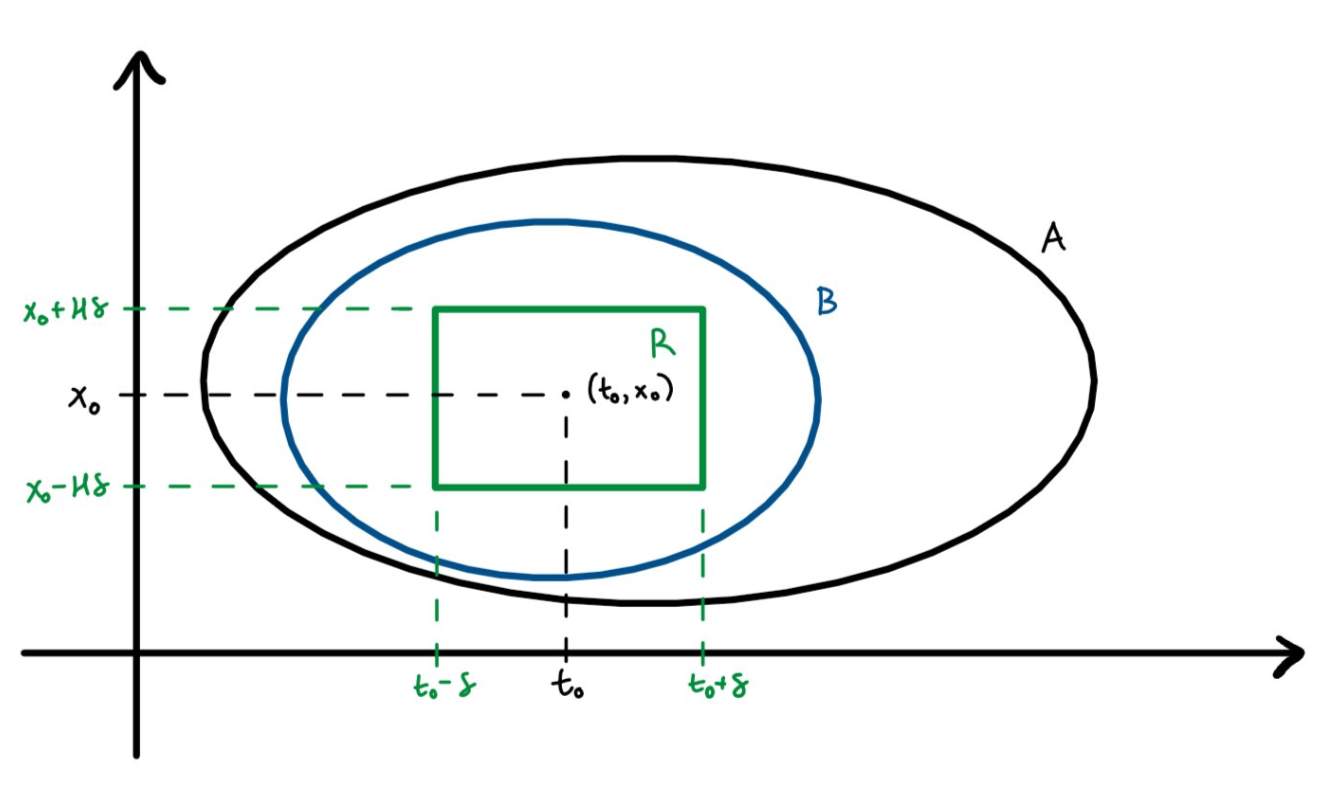
\includegraphics[scale=0.3]{picard}
		\caption{Esquema da demostración.}
	\end{figure}
	
	Definimos o conxunto:
	 \[X=\{\varphi : I=[t_0-\delta, t_0+\delta]\longrightarrow \mathbb{R}^n : \varphi \text{ continua, } ||\varphi(t)-x_0||\leq H \delta \hspace{0,2cm} \forall t \in I  \} \]
	das aplicacións continuas cuxo grafo está en $R$. Dotaremos a este conxunto $ X $ coa seguinte métrica. Dadas $\varphi, \psi \in X$, $d(\varphi, \psi) = sup_{t \in I} \norm{\varphi (t) - \psi (t)}$ (como exercicio probar que é unha métrica). Así temos que:\\
	\[\begin{rcases}
		C(I, \mathbb{R}^n) \text{ espacio métrico completo \footnotemark}\\
		X = B_{C(I, \mathbb{R}^n)} [x_0, H\delta] \subset C(I, \mathbb{R}^n) \text{ cerrado } \\
	\end{rcases} \Rightarrow (X, d) \text{ completo.}\]
	\footnotetext{Un espacio métrico completo es aquel en el que toda sucesión de Cauchy converge a un punto en el mismo conjunto. En la demostración usamos el siguiente resultado: Un subconjunto cerrado de un espacio métrico completo es completo.}
	
	Nótese que $ x_0 $ pode ser entendido como a función constante $ x_0 $, no contexto dun espazo de funcións. Definimos agora:
	\[T:\varphi \in X \longrightarrow T\varphi = x_0 + \int_{t_0}^{t} f(s, \varphi(s))ds\]
	Queremos usar o Teorema \ref{transformada} da transformada contractiva, por tanto, temos que demostrar:
	\begin{enumerate}
		\item $T\varphi \in X$.
		\item $T$ é $\lambda$-contracción.
	\end{enumerate}
	Para ver que $T\varphi \in X$ temos que ver:
	\begin{enumerate}[	i.]
		\item $T\varphi$ continua
		\item $\norm{T\varphi (t) - x_0} \leq H\delta$, $\forall t \in I$
	\end{enumerate}
	En primeiro lugar, temos que:
	\[s \stackrel{g}{\longrightarrow} (s, \varphi (s)) \stackrel{f}{\longrightarrow} f(s, \varphi (s)) \longrightarrow x_0 + \int_{t_0}^{t}f(s,\varphi (s))ds  \]
	polo que $T\varphi$ é continua por composición de funcións continuas. \\
	En segundo lugar, 
	\[\norm{T\varphi - x_0} = \norm{x_0 + \int_{t_0}^{t} f(s, \varphi (s)) ds - x_0} = \norm{\int_{t_0}^{t} f(s, \varphi (s)) ds} \leq \]
	\[\abs{\int_{t_0}^{t} \norm{f(s, \varphi (s))}ds} \leq \abs{\int_{t_0}^{t} H ds} = \abs{H(t - t_0)} = H\abs{t - t_0} \leq H\delta \]
	Vexamos agora que $T$ é unha $\lambda$-contracción, é dicir, $\exists \lambda \in \mathbb{R}$, $0 \leq \lambda < 1$ tal que
	\[d(T\varphi, T\psi) \leq \lambda d(\varphi, \psi) \hspace{0,2cm} \forall \varphi, \psi \in X\]
	Sexan $\varphi, \psi \in X$, \\
	\[d(T\varphi, T\psi) = sup_{t \in I} \norm{T\varphi (t) - T\psi (t)} = sup_{t \in I} \norm{x_0 + \int_{t_0}^{t} f(s, \varphi(s))ds - x_0 - \int_{t_0}^{t} f(s, \psi(s))ds} = \]
	\[sup_{t \in I} \norm{\int_{t_0}^{t} (f(s, \varphi(s)) - f(s, \psi(s)))ds} \leq sup_{t \in I} \abs{\int_{t_0}^{t} \norm{(f(s, \varphi(s)) - f(s, \psi(s)))}ds} \stackrel{f \in L_{loc} (A, x)}{\leq} \] 
	\[sup_{t \in I} \abs{\int_{t_0}^{t} k\norm{\varphi(s) - \psi(s)}ds} \leq sup_{t \in I} \abs{\int_{t_0}^{t} k sup\norm{\varphi(s) - \psi(s)}ds} \leq sup_{t \in I} \abs{\int_{t_0}^{t} k d(\varphi, \psi)ds} = \]
	\[sup_{t \in I} kd(\varphi, \psi)\abs{t - t_0} \leq kd(\varphi, \psi)\delta \leq \lambda d(\varphi, \psi)\]
	Tomando $\lambda = \delta k$, como $\delta < \frac{1}{k}$ temos que $\lambda < 1$. Nótese que podemos aplicar que $ f $ é $ L_{\text{loc}} $ en $ A $ respecto de $ x $ xa que ao ser $ \psi $ e $ \varphi $ funcións de $ X $, están definidas nunha contorna de $ t_0 $ no que $ f $ é lipschitziana, e sempre traballamos con $ t $ dentro desa contorna, por como estamos a construír a proba.
	
	Por tanto, $T$ é $\lambda$-contracción. É dicir, polo Teorema \ref{transformada} da transformada contractiva:
	\[\exists ! \varphi \in X : \varphi \text{ punto fijo de } T\]
	polo que $\varphi (t) = T\varphi (t) = x_0 + \int_{t_0}^{t} f(s, \varphi (s))ds$, e como $\varphi$ continua, cumpre as dúas hipóteses do Teorema \ref{carac-sol} de caracterización de solucións.	

	\begin{figure}[h]
		\centering
		\begin{tikzpicture}
		\draw[->] (-1,0) -- (5,0) node[right] {$t \in \mathbb{R}$}; %eje x, en este caso t
		\draw[->] (0,-0.5) -- (0,3.5) node[above] {$x \in \mathbb{R}^n$};% eje y
		\draw  plot[tension=.7] coordinates {(1,1) (1,2.5) (4,2.5) (4,1) (1,1) }; %conjunto R
		\draw  plot[scale=0.53,shift={(4.3,2.75)},smooth, tension=.7] coordinates {(-3.5,0.5) (-3,2.5) (-1,3.5) (1.5,3) (4,3.5) (5,2.5) (5,0.5) (2.5,-2) (0.5,-1.5) (-3,-2) (-3.5,0.5)}; % conjunto A
		\draw[-] (2.5,0.10) -- (2.5,-0.10) node[below][scale=0.8]{$t_0$}; %t0 y puntos de x
		\draw[-] (1,0.10) -- (1,-0.10) node[below][scale=0.8]{$t_0-\delta$};
		\draw[-] (4,0.10) -- (4,-0.10) node[below][scale=0.8]{$t_0+\delta$};
		\draw[-] (-0.10,1.75) -- (0.10,1.75) node[left=2mm][scale=0.8]{$x_0$}; %x_0 y puntos de y
		\coordinate[label=above:A] (A) at (5.2,2.8); %etiqueta de A
		\coordinate[label=above:R] (R) at (4.2,2.2); %etiqueta de R
		\draw  plot[smooth,tension=.7] coordinates {(1,1.75) (1.5,2.2) (1.7,2) (2.25,2.6) (2.8,0.75) (3.2, 2.6) (3.4, 1.9) (4, 2.3)}; %linea poligonal
		\fill (2.5,1.75)  circle[radius=1pt]; %punto en t0,x_0
		\coordinate[label={[scale=0.6] right:$(t_0,x_0)$}] (p0) at (2.5,1.7); %etiqueta de t0 x0
		\end{tikzpicture}
		\caption{Situación na que o grafo non está en $ R $.} \label{M1}
	\end{figure}
	¿Podería existir unha función que fose solución pasando polo punto e que o grafo non estea en $ R $? Probemos que non.
	\begin{adjustwidth}{1cm}{}
		Vexamos que se $ \psi : I \longrightarrow\mathbb{R}^n $ solución de $ x'=f(t,x) $ pasando por $ (t_0,x_0) $, entón $ \psi \in X $, é dicir, $ ||\psi(t)-x_0||\leq H\delta \ \forall t \in I $.
		
		Probémoslo por redución ao absurdo. Supoñamos que $ \exists t_1\in I : ||\psi(t_1)-x_0||>H\delta$, por ser $ \psi $ continua $ \exists t_2\in (t_0,t_1) $ no cal $ ||\psi(t_2)-x_0||=H\delta $.
		
		Sexa $ t^* = \inf \{t : ||\psi(t)-x_0||=H\delta, t>t_0 \} \Rightarrow ||\psi(t^*)-\psi(t_0)||=H\delta$, con $ \psi(t_0)=x_0 $.
		
		Por outra banda, $ ||\psi(t^*)-\psi(t_0)||\leq ||\psi'(t)||\cdot |t^*-t_0|<H\delta $, o cal é unha contradición.
	\end{adjustwidth}
	
	¿Podería existir outra solución distinta que pasase polo punto?
	\begin{adjustwidth}{1cm}{}
		Vexamos que isto tampouco pode pasar. Supoñamos que $ \varphi_1: I_1\longrightarrow\mathbb{R}^n, \varphi_2:I_2 \longrightarrow \mathbb{R}^n $ son solucións de $ x'=f(t,x) $ pasando por $ (t_0,x_0) $ e $ \exists t\in I_1\cap I_2 : \varphi_1(t)\neq \varphi_2(t) $.
		
		Sexa por exemplo $ t>t_0 $. Sexa $ t_1=\inf \{t \in I_1\cap I_2 :t>t_0, \varphi_1(t)\neq \varphi_2(t)  \} $.
		
		Por definición de ínfimo $ \varphi_1(t)=\varphi_2(t) \ \forall t \in [t_0, t_1) $ e ademais $ \varphi_1(t_1)=\lim\limits_{t\to t_1^-} \varphi_1(t) $ por ser $ \varphi_1 $ continua.
		
		$ \varphi_1(t_1)=\lim\limits_{t\to t_1^-} \varphi_1(t)=\lim\limits_{t\to t_1^-} \varphi_2(t)= \varphi_2(t_1) $.
		
		Entón $ \varphi_1(t)=\varphi_2(t) \ \forall t \in [t_0,t_1], \varphi_1(t_1)=\varphi_2(t_1)=x_1 $.
		
		Facemos en $ (t_1, x_1) $ o mesmo que en $ (t_0,x_0) $ (construímos o rectángulo, etc...) e chegamos a que en $ (t_1-\delta_1, t_1+\delta _1), \varphi_1(t)=\varphi_2(t) $ e isto NON é posible xa que, por construción, $ t_1=\inf \{t\in I_1\cap I_2 : t>t_0, \varphi_1(t)\neq \varphi_2(t)\} $.
	\end{adjustwidth}
\end{proof}

\section{Tema 3.}
\begin{example}
	Dada a ecuación diferencial $ x'=x^2 $, pasando polo punto $ x(1)=1 $, temos que $ x(t)=\frac{-1}{t} $ é solución. $ x'(t)=x(t)^2 $ é unha ecuación exposta para todo $ t \in \mathbb{R} $, pero $ x(t)=\frac{-1}{t} $ está definida para $ t \in \mathbb{R}-\{0\} $.
	
	Entón temos que dependendo das condicións iniciais a solución da EDO estará definida para $ t\in (0,\infty) $ o $ t\in (-\infty,0) $.
	
	Fixémonos en dous aspectos: coas condicións iniciais propostas, $ x(1)=1 $, podemos definir a solución no intervalo $ (0,3) $. Con todo, esta solución podería ser prolongada a un dominio de $ (0,\infty) $, e a posibilidade desta prolongación será obxecto de estudo.
	
	Por outra banda, vemos que ao cambiar as condicións iniciais (por exemplo, $ x_0=-0.0001 $ o $ x_0=0.00001 $), a solución da ecuación non é a mesma e noutros caso, podería variar a súa expresión analítica. Interesaranos que para variacións ''pequenas'' das condicións iniciais, a solución da ecuación non varíe ''case nada''.
\end{example}

\begin{note}
	Os teoremas de Cauchy-Peano e Picard-Lipschitz definen existencia e unicidade de solucións a nivel local, nunha contorna arbitrariamente pequeno. Son preguntas naturais: \begin{itemize}
		\item ¿Cal é o maior intervalo no que están definidas esas solucións?
		\item ¿Ata onde podo prolongar as mesmas?
	\end{itemize}
\end{note}
\subsection{Prolongación de solucións. Solucións maximais.}
\begin{definition}
	Sexan $ A $ un aberto de $ \mathbb{R}^{n+1} $ e $ f $ a aplicación continua $ f:(t,x)\in A\subset \mathbb{R}\times \mathbb{R}^n \longrightarrow f(t,x)\in \mathbb{R}^n $, con $  x'=f(t,x) $ a súa ecuación diferencial asociada. 
	
	Sexan ademais $ \varphi_1:I_1\longrightarrow \mathbb{R} $ e  $ \varphi_2:I_2\longrightarrow \mathbb{R} $ solucións da devandita ecuación diferencial. Diremos que $ \varphi_2 $ é unha \iindex{prolongación} de $ \varphi_1 $ se:
	\begin{enumerate}
		\item $ I_1\subseteq I_2 $
		\item $ \varphi_1(t) =\varphi_2(t) \ \forall t \in I_1$
	\end{enumerate}

	Ademais, se $ I_1 \varsubsetneq I_2 $ diremos que $ \varphi_2 $ é unha \iindex{prolongación propia} de $ \varphi_1 $.
\end{definition}
\begin{note}
	Unha solución é prolongación de si mesma, pero non é prolongación propia.
\end{note}
\begin{definition}
	Se $ \varphi $ é solución dunha ecuación diferencial, diremos que $ \varphi $ é unha \iindex{solución maximal} se non admite prolongación propia. Neste caso, o intervalo de definición é chamado \iindex{intervalo maximal}.
\end{definition}
\begin{lemma}[Lema de Zorn]
	Todo conxunto parcialmente ordenado non baleiro, no que toda cadea (subconjunto parcialmente ordenado) admite cota superior, contén elementos maximales.
\end{lemma}
\begin{theorem}
	Sexan $ A $ un aberto de $ \mathbb{R}^{n+1} $ e $ f $ a aplicación continua $ f:(t,x)\in A\subset \mathbb{R}\times \mathbb{R}^n \longrightarrow f(t,x)\in \mathbb{R}^n $, con $  x'=f(t,x) $ a súa ecuación diferencial asociada. 
	
	Dado $ (t_0,x_0)\in A $, existe unha solución maximal da ecuación diferencial que pasa por $ (t_0,x_0) $.
	
\end{theorem}
\begin{proof} \ \\	
	Faremos uso do lema de Zorn. Representaremos as solucións da ecuación diferencial mediante o par $ (I,\varphi) $ onde $ \varphi $ é a solución e $ I $ o seu intervalo de definición.
	
	Neste conxunto definimos a relación de orde parcial "ser prolongación". Se $ \psi $ é prolongación de $ \varphi $:
	\[ (I,\varphi)\leq (J,\psi)\Leftrightarrow I\subseteq J, \varphi(t)=\psi(t) \ \forall t \in I \]
	Agora, sexa $ (I_0,\varphi_0) $ solución de $ x'=f(t,x) $ e vexamos que se pode prolongar ata unha solución maximal.
	
	Traballamos só con solucións que sexan prolongación de $ \varphi_0 $. É un conxunto non baleiro, xa que $ (I_0,\varphi_0) $ é prolongación de se mesmo. Utilizamos a relación de orde parcial definida anteriormente e comprobamos que se cumpre a outra hipótese do lema de Zorn:
	
	Sexa $ \{(I_j,\varphi_j) \}_{j\in I} $ unha cadea dese conxunto e vexamos que admite cota superior. Sexa $ \varphi $ a función definida en $ I=\bigcup_{j\in I}I_j $ mediante $ \varphi(t)=\varphi_j(t) \ \forall j \in I $. $ \varphi $ é claramente cota superior da cadea.
	
	Por tanto, polo lema de Zorn, existen elementos maximales que son as solucións maximales que prolongan a $ \varphi_0 $.	
\end{proof}
\begin{definition}
	Sexan $ A $ un aberto de $ \mathbb{R}^{n+1} $ e $ f $ a aplicación continua $ f:(t,x)\in A\subset \mathbb{R}\times \mathbb{R}^n \longrightarrow f(t,x)\in \mathbb{R}^n $, con $  x'=f(t,x) $ a súa ecuación diferencial asociada. 
	
	Sexan $ \varphi_1:(a,b)\longrightarrow \mathbb{R}^n $ e $ \varphi_2:(c,d)\longrightarrow \mathbb{R}^n $ solucións da devandita ecuación diferencial. Se $ \varphi_2 $ é unha prolongación de $ \varphi_1 $ e $ b\in(c,d) $, diremos que $ \varphi_2 $ é \iindex{prolongación de $ \varphi_1 $ a través de $ b $}.
\end{definition}
\begin{definition}[Xeneral]
	Sexan $ A $ un aberto de $ \mathbb{R}^{n+1} $ e $ f $ a aplicación continua $ f:(t,x)\in A\subset \mathbb{R}\times \mathbb{R}^n \longrightarrow f(t,x)\in \mathbb{R}^n $, con $  x'=f(t,x) $ a súa ecuación diferencial asociada. 
	
	Sexan $ \varphi_1:I_1\longrightarrow \mathbb{R}^n $ e $ \varphi_2:I_2\longrightarrow \mathbb{R}^n $ solucións da devandita ecuación diferencial. Se $ \varphi_2 $ é unha prolongación de $ \varphi_1 $ e existe $ q\in \text{Fr}(I_1) $ tal que $ q\in \mathring{I_2}$, diremos que $ \varphi_2 $ é \iindex{prolongación de $ \varphi_1 $ a través de $ q $}.
\end{definition}
\begin{theorem}[Teorema de prolongación] \label{prolTh}
	Sexan $ A $ un aberto de $ \mathbb{R}^{n+1} $ e $ f $ a aplicación continua $ f:(t,x)\in A\subset \mathbb{R}\times \mathbb{R}^n \longrightarrow f(t,x)\in \mathbb{R}^n $, con $  x'=f(t,x) $ a súa ecuación diferencial asociada. 
	
	Ademais destas condicións habituais, pediremos que $ f\in L_{\text{loc}}(A,x) $, é dicir, que $ f $ sexa lipschitziana localmente.
	
	Se $ \varphi:(a,b)\longrightarrow\mathbb{R}^n $ é solución da ecuación diferencial anterior, entón;
	\begin{enumerate}[\quad i)]
		\item $ \varphi $ prolongable a través de $ b \Leftrightarrow \exists \lim\limits_{t\to b^-}\varphi(t)=p, \text{ con } (b,p) \in A $
		\item $ \varphi $ prolongable a través de $ a \Leftrightarrow \exists \lim\limits_{t\to a^+}\varphi(t)=q, \text{ con } (a,q) \in A $
	\end{enumerate}
\end{theorem}


\begin{proof}\ 
	\begin{enumerate} [\quad i)]
		\item "$\Rightarrow$" \\
		Se $\varphi$ prolongable a través de $b$, entón $\exists \varphi_2 : (a, d) \longrightarrow \mathbb{R}^n$ prolongación de $\varphi$ (é dicir, $\varphi_2 = \varphi$ $\forall t \in (a, b)$, $b \in (a, b)$). Por ser $\varphi_2$ solución, $\varphi_2$ é continua pola esquerda en $t = b$, polo que:
		\[\lim\limits_{t \to b^-} \varphi_2(t) = \varphi_2(b) \text{, } \lim\limits_{t \to b^-} \varphi_2(t) = \lim\limits_{t \to b^-} \varphi(t)\]
		e temos entón que:
		\[\lim\limits_{t \to b^-} \varphi(t) = \varphi_2(b)\]
		Ademais, $(b, \varphi(b)) \in A$ por ser $\varphi_2$ solución. \\
		"$\Leftarrow$" \\
		Supoñemos que:
		\[\exists \lim\limits_{t \to b^-} \varphi(t) = p \text{, } (b, p) \in A\]
		Sexa $\overline{B} = B((b, p), r) \subset A$ con $f$ acoutada en $\overline{B}$ e $f \in L_k (B, x)$. Tomamos $0 < \delta < min\{\frac{r}{2}, \frac{r/2}{H}, \frac{1}{k}\}$, sendo $H$ cota de $f$.
		
		\begin{figure}[h]
			\centering
			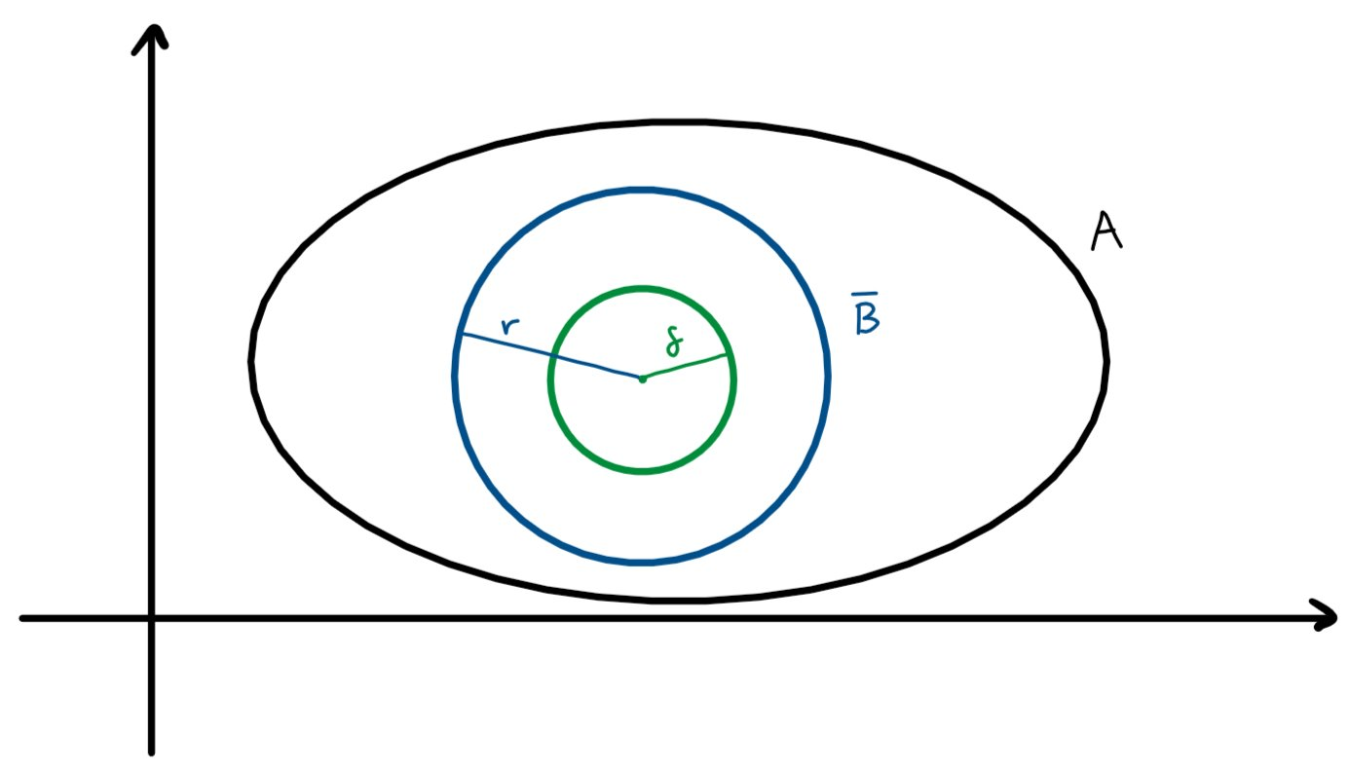
\includegraphics[scale=0.3]{prolongacion}
			\caption{Conxuntos implicados.}
		\end{figure}
		
		Como $\lim\limits_{t \to b^-} \varphi (t) = p$ e, por ser continua, $ \varphi $ é secuencialmente continua, existe unha sucesión $\{t_n\} \longrightarrow b^-$ tal que $\{\varphi(t_n)\} \longrightarrow p$. Eliximos entón un $n_0 \in \mathbb{N}$ tal que $\abs{t_{n_0} - b} < \delta$ e $(t_{n_0}, \varphi (t_{n_0})) \in \overline{B}$. Para a condición inicial $(t_{n_0}, \varphi (t_{n_0}))$ existe unha solución única pasando polo punto definido en $[t_{n_0} - \delta, t_{n_0} + \delta]$ que denoto $\overline{\varphi}$. Entón a función:
		\[\psi: (a, t_{n_0} + \delta] \longrightarrow \psi (t) = \begin{cases}
		\varphi(t) &t \in (a, b) \\ 
		\overline{\varphi} (t) &t \in [b, t_{n_0} + \delta).
		\end{cases}\]
		Así, temos que $\psi$ é solución de $x' = f(t. x)$ e, de feito, $\psi$ prolonga a $\varphi$ a través de $b$.
		\item Análogo.
	\end{enumerate} 
\end{proof}
\begin{observation}
	En primeiro lugar, a afirmación $i)$ é equivalente a dicir:
	\[\exists \{t_m\} \longrightarrow b^- : \exists \lim\limits_{t_n \to b^-} \varphi(t_n) = p \hspace{0.2cm} (b, p) \in A\]
	Chega traballar cunha sucesión. Ademais, non é necesario pedir que $f \in L_{loc}(A, x)$, simplemente sen ela non podemos concluír a unicidade e a demostración sería moito máis complicada.
\end{observation}
\begin{corollary}
	Se $A$ está acoutado, a solución pódese prolongar ata a fronteira.
\end{corollary}
\begin{theorem}[Teorema da banda]\label{banda} \ \\ 
	Dada a ecuación diferencial $x' = f(t, x)$, con $f: (t, x) \in \mathbb{R} \times \mathbb{R}^n \longrightarrow f(t, x) \in \mathbb{R}^n$ sendo $A = (a, b) \times \mathbb{R}^n$. Se se cumpre unha das seguintes condicións:
	\begin{enumerate}
		\item  $f$ continua en $A$, $f \in L_k (A, x)$.
		\item  $f$ continua e acoutada en $A$ ($f \in L_{loc} (A, x)$).
	\end{enumerate}
	
	\begin{figure}[h]
		\centering
		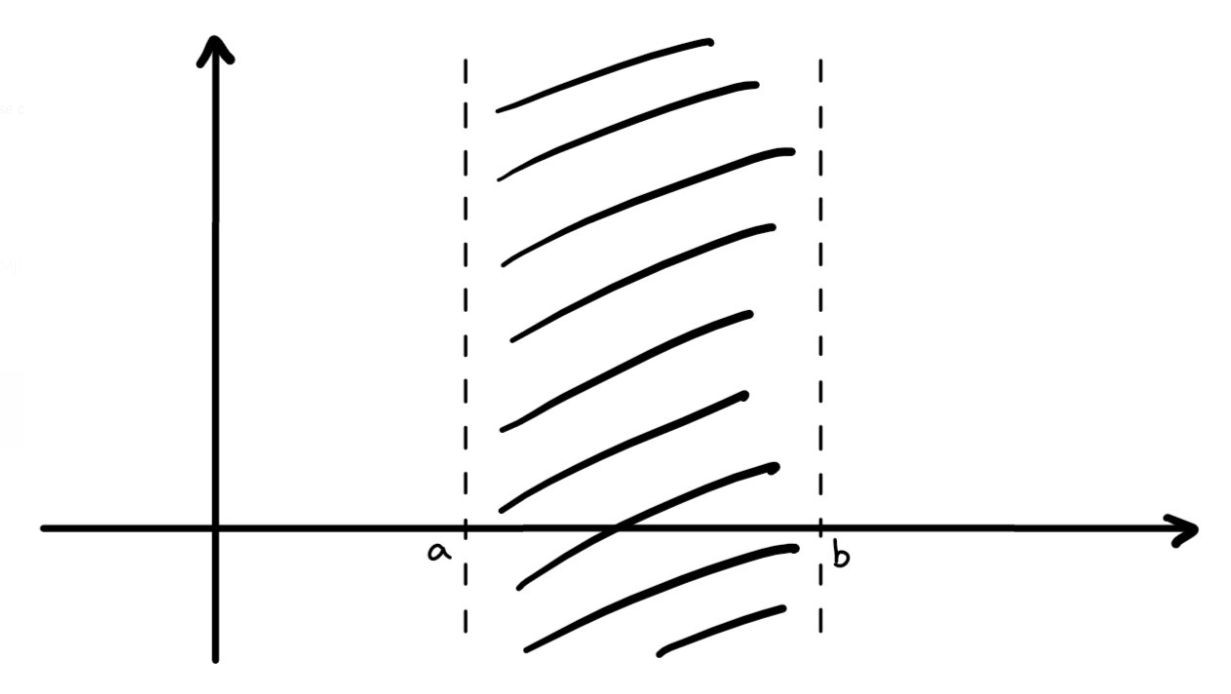
\includegraphics[scale=0.3]{banda}
		\caption{Teorema da banda.}
	\end{figure}
	
	entón, fixado $(t_0, x_0) \in (a, b) \times \mathbb{R}^n$, a solución maximal que pasa por el está definida en $(a, b)$.
\end{theorem}
\begin{observation} \ 
	\begin{enumerate}
		\item Non é necesario pedir $f \in L_{loc} (A, x)$.
		\item $a$, $b$ non teñen porque ser finitos, é dicir, pode tratarse de intervalos da forma $(- \infty, b)$.
	\end{enumerate}
\end{observation}
\begin{theorem}[Teorema da banda pechada] \label{bandacerrada} \ \\
	Dada a ecuación diferencial $x' = f(t, x)$, con $f: [a, b] \times \mathbb{R}^n \longrightarrow \mathbb{R}^n$. Se se cumpre unha das seguintes condicións:
	\begin{enumerate}
		\item $f$ continua en $A = [a, b] \times \mathbb{R}^n$, $f \in L_k (A, x)$.
		\item $f$ continua en $A$, $f \in L_{loc} (A, x)$.
	\end{enumerate}
	entón, fixado $(t_0, x_0) \in A$ a solución maximal pasando por ese punto está definida en $[a, b]$. 
\end{theorem}
\begin{proof}\ \\
	Definimos a seguinte función, onde $A \subset (c, d) \times \mathbb{R}^n$:
	\[g: (t, x) \in (c, d) \times \mathbb{R}^n \longrightarrow g(t, x) = \begin{cases}
	f(a, x), &t \in (c, a] \\
	f(t, x), &t \in [a, b] \\
	f(b, x), &t \in [b, d)
	\end{cases}\]
	e con $g$ continua. Esta función verifica as hipóteses do teorema anterior en $(c, d) \times \mathbb{R}^n$ xa que:
	\begin{enumerate}[-]
		\item Se $f \in L_k(A, x) \Rightarrow g \in L_k ((c, d) \times \mathbb{R}^n)$
		\item Se $f$ acoutado e $f \in L_{loc} (A, x)$, entón $g$ acoutada e $g \in L_{loc} ((c, d) \times \mathbb{R}^n, x)$.
	\end{enumerate}
	Por tanto, fixado $(t_0, x_0) \in A \subset (c, d) \times \mathbb{R}^n$ existe a solución maximal pasando por $(t_0, x_0)$ e definida en $(c, d)$. Por tanto, $\varphi = \psi|_{[a, b]}$ é a solución maximal de $x' = f(t, x)$ pasando por $(t_0, x_0)$.
	
	\begin{figure}[h]
		\centering
		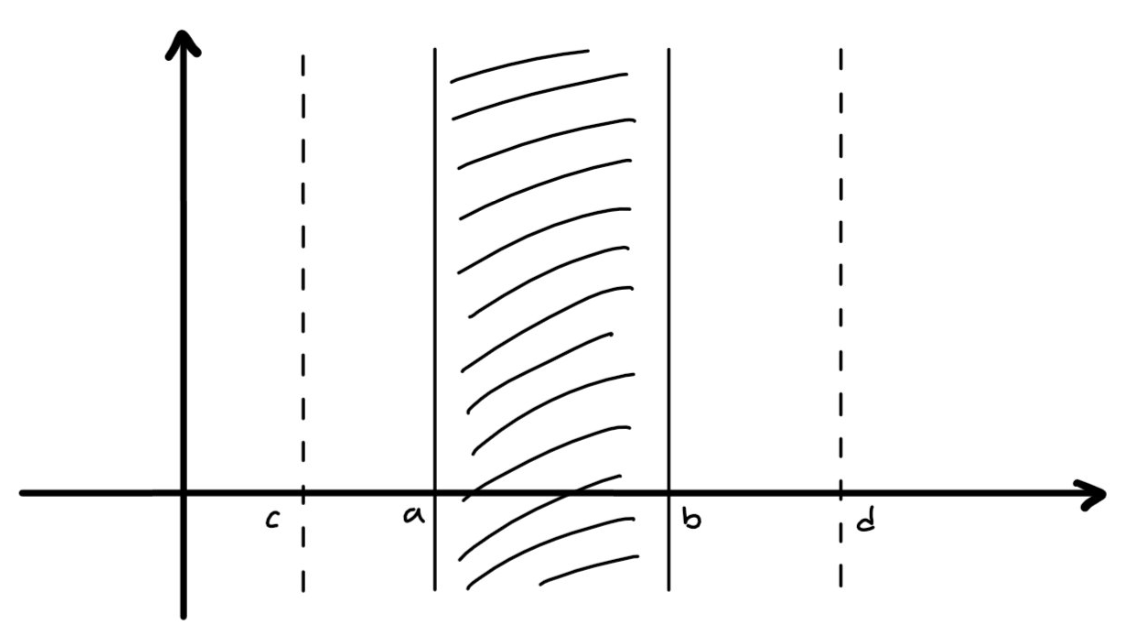
\includegraphics[scale=0.3]{banda_cerrada}
		\caption{Teorema da banda pechada.}
	\end{figure}
	\end{proof}

\begin{proposition}
	Sexan $ A $ un aberto de $ \mathbb{R}^{n+1} $ e $ f $ a aplicación continua $ f:(t,x)\in A\subset \mathbb{R}\times \mathbb{R}^n \longrightarrow f(t,x)\in \mathbb{R}^n $, con $  x'=f(t,x) $ a súa ecuación diferencial asociada. 
	
	Se $ \varphi_1, \varphi_2 $ son solucións da ecuación, definidas en $ [a, t_0]$ e $ [t_0,b] $, respectivamente, e ademais $ \varphi_1(t_0)=\varphi_2(t_0) $, entón $ \varphi $ definida en $ [a,b] $ como:
	\[ \varphi(t)=\begin{cases}
	\varphi_1(t), \quad t\in [a,t_0]\\
	\varphi_2(t), \quad t\in [t_0,b]
	\end{cases} \]
	é solución da ecuación diferencial.
\end{proposition}
\begin{proof}\ \\
	Vexamos que $ \varphi $ é solución por definición:
	\begin{enumerate}[\quad i)]
		\item $ (t,\varphi(t))\in A \ \forall t \in [a,b], $ xa que $ \begin{cases}
		\forall t\in [a,t_0] \quad (t, \varphi_1(t)) \in A, \text{ xa que }\varphi_1 \text{ é solución.}\\
		\forall t\in [t_0,b] \quad (t, \varphi_2(t)) \in A, \text{ xa que }\varphi_2 \text{ é solución.}\\
		\text{Ademais, } \varphi_1(t)=\varphi_2(t).
		\end{cases}$
		\item $ \forall t \in [a,t_0) \ \exists \varphi_1'(t)$
		
		$ \forall t \in [t_0,b) \ \exists \varphi_2'(t) $
		
		Vexamos se existe a derivada en $ t_0 $, utilizando a continuidade de $ \varphi_1 $ e $ \varphi_2 $:
		\[ \lim\limits_{t \to t_0^-} \varphi'_1(t)=\lim\limits_{t \to t_0^-} f(t, \varphi_1(t))=f(t_0,\varphi_1(t_0)) \]
		\[ \lim\limits_{t \to t_0^+} \varphi'_2(t)=\lim\limits_{t \to t_0^+} f(t, \varphi_2(t))=f(t_0,\varphi_2(t_0)) \]
		Como $ \varphi_1(t_0)=\varphi_2(t_0) \Rightarrow \lim\limits_{t \to t_0^-} \varphi'(t)=\lim\limits_{t \to t_0^+} \varphi'(t)$, e $\varphi $ continua en $ t_0 $, entón efectivamente existe $ \varphi'(t_0) $.
		\item Inmediata visto o anterior.
	\end{enumerate} 
\end{proof}
\begin{proposition}
	Sexan $ A $ un aberto de $ \mathbb{R}^{n+1} $ e $ f $ a aplicación continua $ f:(t,x)\in A\subset \mathbb{R}\times \mathbb{R}^n \longrightarrow f(t,x)\in \mathbb{R}^n $, con $  x'=f(t,x) $ a súa ecuación diferencial asociada. 
	
	Entón, toda solución maximal está definida nun aberto.
\end{proposition}
\begin{proof}\ \\
	Probémolo por redución ao absurdo. Supoñamos que está definida nun intervalo da forma $ (a,b] $.
	Como $ A $ é aberto, $ (b,\varphi(b))\in A \Rightarrow (b, \varphi(b)) \in \mathring{A} $.
	
	Estamos nas hipóteses do Teorema de Cauchy-Peano. Por tanto, pasando por $ (b, \varphi(b)) $ existe solución. Podemos construír unha prolongación que sexa solución (polo teorema \ref{prolTh} apartado i) e entón non é maximal.
\end{proof}


\section{Tema 4.}
\subsection{Métodos elementales de integración das ecuacións de primeira orde.}
\subsubsection{EDOs de variables separadas.}
Son ecuacións da forma $ x'=\frac{\partial x}{\partial t}=h(t)g(x) $, con $ h:I_1\longrightarrow\mathbb{R} $ e $ g:I_2\longrightarrow\mathbb{R} $ continuas. 
\paragraph{Xustificación da existencia e unicidade da solución} \ \\
Como $ A=I_1\times I_2 $ debe ser aberto, os intervalos deben ser abertos. Pola continuidade de $ h $ e $ g $ dedúcese a continuidade de $ f(t,x)=h(t)g(x) $, o que nos permite aplicar o teorema \ref{cauchy-peano} de existencia de solución.

Se ademais queremos a unicidade da mesma, necesitamos que $ f $ sexa localmente lipschitziana respecto a $ x $ para poder aplicar o teorema \ref{picard}, é dicir, que $ g $ sexa localmente lipschitziana respecto a $ x $. Tal e como vimos no teorema \ref{lloc_suf}, é suficiente que $ g\in C'(I_2) $.

Nestas condicións, fixado $ (t_0,x_0)\in I_1\times I_2=A $, comprobemos que cumprimos as hipóteses do teorema \ref{picard}:
\begin{enumerate}[i)]
	\item $ I_1\times I_2 $ aberto.
	\item $ f(t,x)=h(t)g(x) $ continua por produto de funcións continuas.
	\item $ f\in L_{loc} (A,x) $ xa que $ g\in L_{loc}(I_2,x) $
\end{enumerate}

\paragraph{Método de resolución}
\begin{enumerate}
	\item $ \frac{1}{g(x)}\cdot\frac{\partial x}{\partial t}=h(t) $
	\item $ \frac{1}{g(x)}\cdot\partial x=h(t)\partial t $
	\item $ \int \frac{1}{g(x)} \partial x= \int h(t) \partial t \Rightarrow G(x)+c_1=H(t)+c_2 \Rightarrow G(x)=H(t)+c$
\end{enumerate}
Se se pide a solución pasando por $ (t_0,x_0) $, achamos a $ c $ que cumpre $ G(x_0)=H(t_0)+c $, é dicir, $ G(x)=H(t)+G(x_0)-H(t_0) \Rightarrow G(x)-G(x_0)=H(t)-H(t_0)$.

Outra forma de chegar a este resultado é observar:
\[ \int_{x_0}^{x} \frac{1}{g(x)} \partial x= \int_{t_0}^{t} h(t) \partial t \Rightarrow G(x)-G(x_0)=H(t)-H(t_0)\]

Nótese que se $ g(x_0)=0 $, entón $ x(t)=x_0 $ é a solución.

\paragraph{Xustificación de que a solución está ben definida}
\begin{theorem}
	Sexa $ M:(t,x)\longrightarrow M(t,x)=G(x)-G(x_0)-(H(t)-H(t_0)) $. Entón $ M(t,x) $ define implicitamente unha solución de $ x'=f(t,x)=h(t)g(x) $, é dicir, a expresión obtida no método de resolución é correcta e a solución vén dada por $ M(t,x)=0 $.
\end{theorem}
\begin{proof}
	Probémoslo utilizando o teorema da implícita. Nótese que 
	\[  M(t,x)=G(x)-G(x_0)-(H(t)-H(t_0))= \int_{x_0}^{x} \frac{1}{g(x)} \partial x- \int_{t_0}^{t} h(t) \partial t \]
	Comprobamos as hipóteses:
	\begin{enumerate}
		\item $ M\in C'(A) $, xa que $ h $ e $ g $ continuas.
		\item $ M(t_0,x_0)=0 $
		\item $ \frac{\partial M}{\partial x}(t_0,x_0)=\frac{1}{g(x_0)}\neq 0 $.
	\end{enumerate}
	Como se cumpren as hipóteses, o teorema da implícita asegúranos que existen $ \varepsilon_{t_0} $ contorna de $ t_0 $, $ \varepsilon_{x_0} $ contorna de $ x_0 $ e $ x:t\in\varepsilon_{t_0}\longrightarrow x(t)\in\varepsilon_{x_0}$. Ademais, dinos que $ x(t) $ cumpre:
	\begin{enumerate}
		\item $ x $ continua na contorna.
		\item $ x(t_0)=x_0 $.
		\item $ M(t,x(t))=0 $ para todo $ t\in \varepsilon_{t_0} $, e $ x(t) $ é a única solución de $ M(t,x(t))=0 $.
		\item $ D x(t)=-[D_x M(t,x(t))]^{-1}D_tM(t,x(t)) $. É dicir:
		\[ Dx(t)=x'(t)=\frac{\partial x}{\partial t}= -[\frac{1}{g(x)}]^{-1}(-h(t))=h(t)g(x)=f(t,x) \]
	\end{enumerate}
	Polo que efectivamente, a función $ x(t) $ definida implicitamente cumpre as condicións para ser solución da ecuación diferencial.
\end{proof}
\subsubsection{EDOs homoxéneas.}
Son ecuacións da forma $ x'=g(\frac{x}{t}), $ ou ben $ x'=\frac{f(t,x)}{h(t,x)} $, con $ f,h $ funcións homoxéneas do mesmo grao.
\begin{definition}
	Dicimos que $ f $ é unha \iindex{función homoxénea de grado $ k $} se $ \forall r \in \mathbb{R}, f(rt,rx)=r^kf(t,x)$.
\end{definition}
\paragraph{Método de resolución} \ \\
Sexan $ f,h $ homoxéneas do mesmo grao. Todas as EDOs homoxéneas pódense reducir a $ x'=g(\frac{x}{t})$.
Redución de  $ x'=\frac{f(t,x)}{h(t,x)} $, tomando $ r=\frac{1}{t} $:
	\[ x'= \frac{f(t,x)}{h(t,x)}=\frac{(\frac{1}{t})^kf(t,x)}{(\frac{1}{t})^kh(t,x)}=\frac{f((\frac{1}{t})t,\frac{x}{t})}{h((\frac{1}{t})t,\frac{x}{t})}=\frac{f(1,\frac{x}{t})}{h(1,\frac{x}{t})}=g(\frac{x}{t})\]
	Unha vez temos a ecuación na forma $ x'=g(\frac{x}{t}) $:
	\begin{enumerate}
		\item $ \frac{x}{t}=u\Rightarrow x=u\cdot t $.
		\item Derivando a expresión anterior respecto a $t,\  x'(t)=u(t)+tu'(t)=g(u) \Rightarrow tu'(t)=g(u)-u(t) $
		\item Resolver $ u'(t)=\frac{g(u)-u}{t} $, que é unha EDO de variables separadas en $ u $ e $ t $.
		\item Desfacer o cambio de variable, tendo en conta que $ u=\frac{x}{t} $.
	\end{enumerate}

\subsubsection{EDOs reducibles a homoxéneas.}
Son ecuacións da forma \[ x'=f(\frac{at+bx+c}{mt+nx+p}) \]con $ a,b,c,m,n,p \in \mathbb{R} $.
\paragraph{Método de resolución} \ \\
Para resolvelas, consideramos a ecuación como o cociente de dúas rectas no plano e razoamos a súa posición relativa para reducir a ecuación a un tipo xa coñecido:
\begin{align*}
r&:at+bx+c=0\\
l&:mt+nx+p=0
\end{align*}
Por casos, as rectas pasan pola orixe?:
\begin{enumerate}[\quad i)]
	\item $ c=p=0 $, é dicir, as dúas pasan pola orixe.
	\[ x'=f(\frac{at+bx}{mt+nx})=f(\frac{a+b(\frac{x}{t})}{m+n(\frac{x}{t})}) \text{ homoxénea.} \]
	\item $ c $ e $ p $ non son ambos os nulos.
	\begin{enumerate}
		\item $ r $ e $ l $ córtanse noutro punto. No apartado anterior vimos que se se cortaban noutro punto era homoxénea. Podemos trasladar os eixos ao momento de corte aplicando un cambio de variable e repetir o razoamento anterior.
		
		\begin{figure}[h]
			\centering
			\begin{tikzpicture}[x=0.75pt,y=0.75pt,yscale=-1,xscale=1]	
			%Shape: Axis 2D [id:dp4031260299087579] 
			\draw[line width=0.75pt]   (163,207.7) -- (333.5,207.7)(180.05,70) -- (180.05,223) (326.5,202.7) -- (333.5,207.7) -- (326.5,212.7) (175.05,77) -- (180.05,70) -- (185.05,77)  ;
			%Straight Lines [id:da2069863440207952] 
			\draw [line width=0.75pt]    (230.5,73) -- (273.5,219) ;
			
			%Straight Lines [id:da7364525271296537] 
			\draw[line width=0.75pt]    (167.5,152) -- (318.5,78) ;
			
			%Shape: Circle [id:dp6288291967071182] 
			\draw  [fill={rgb, 255:red, 0; green, 0; blue, 0 }  ,fill opacity=1 ] (240.83,115) .. controls (240.83,113.8) and (241.8,112.83) .. (243,112.83) .. controls (244.2,112.83) and (245.17,113.8) .. (245.17,115) .. controls (245.17,116.2) and (244.2,117.17) .. (243,117.17) .. controls (241.8,117.17) and (240.83,116.2) .. (240.83,115) -- cycle ;
			
			% Text Node
			\draw (268,123.67) node [scale=0.9] [align=left] {$\displaystyle ( \alpha ,\beta )$};
			% Text Node
			\draw (319,89.67) node  [align=left] {$\displaystyle l$};
			% Text Node
			\draw (229,88.67) node  [align=left] {$\displaystyle r$};
			\end{tikzpicture}
			\caption{Cambio de eixos.}
		\end{figure}
		
		$ (t,x) = (\alpha,\beta)+(s,y) $, polo que $ \begin{cases}
		t=\alpha+s\\
		s=\beta+y
		\end{cases} $
		
		Ademais, como \[  x'=\frac{\partial x}{\partial t}=\frac{\partial (\beta+y)}{\partial t}=\frac{\partial y}{\partial s}\frac{\partial s}{\partial t}=\frac{\partial y}{\partial s}   \]temos:
		
		\[  x'=\frac{\partial y}{\partial s}= f(\frac{a(\alpha+s)+b(\beta+y)+c}{m(\alpha+s)+n(\beta+y)+p})= f(\frac{as+by+a\alpha+b\beta+c}{ms+ny+m\alpha+n\beta+p})  \]
		Pero como as rectas córtanse en $ (\alpha, \beta) $, temos que $ a\alpha+b\beta+c=0 $ e $ m\alpha+n\beta+p=0 $. É dicir:
		\[ x'=f(\frac{as+by}{ms+ny})=f(\frac{a+b(\frac{y}{s})}{m+n(\frac{y}{s})})=g(\frac{y}{s}) \text{ homoxénea.}\]
		\item $ r $ e $ l $ son paralelas. Neste caso, que sexan paralelas quere dicir que $ (a,b)=k(m,n) $, xa que a súa vector dirección debe ser proporcional. Por tanto,
		\[ x'=f(\frac{at+bx+c}{mt+nx+p})=f(\frac{kmt+knx+c}{mt+nx+p})=f(\frac{k(mt+nx)+c}{(mt+nx)+p})\]
		Realizando o cambio de variable $ z=mt+nx $:
		\[ \frac{\partial z}{\partial t}=z'=m+nx'=m+nf(\frac{kz+c}{z+p}) \text{ ecuación de variables separadas.} \]
		Nótese que é necesario desfacer o cambio de variable tras a resolución.
	\end{enumerate}
\end{enumerate}
\subsubsection{EDOs lineales.}
Son ecuacións da forma $ x'=a(t)x+b(t) $ con $ a,b: I\in\mathbb{R}\longrightarrow \mathbb{R} $ continuas.
\begin{definition}\ 
	\begin{enumerate}[\quad i)]
		\item Se $ b(t)=0 $, é unha \iindex{EDO lineal homoxénea}.
		\item Se $ b(t)\neq 0 $, para algún $ t\in I $, é unha \iindex{EDO lineal non homoxénea ou completa}.
	\end{enumerate}
\end{definition}
\paragraph{Método de resolución} \ \\
Distinguiremos segundo o tipo de ecuación lineal:
\begin{enumerate}[\quad i)]
	\item Ecuación lineal homoxénea, $ x'=a(t)x $. É unha ecuación de variables separadas.
	\[ \int\frac{1}{x}dx=\int a(t)dt\Rightarrow\ln\abs{x}=\int a(t)dt+k, \ k\in\mathbb{R}\Rightarrow\abs{x}=e^{k+\int a(t)dt}=k'e^{\int a(t)dt}, \ k'>0 \]
	\[ \abs{x}=\begin{cases}
	\ \ x=k'e^{\int a(t)dt}, \ x>0, k'>0\\
	-x=k'e^{\int a(t)dt}, \ x<0, k'>0
	\end{cases}\Rightarrow x=ce^{\int a(t)dt}, \ c\in \mathbb{R}  \]
	Para achar unha solución particular, substitúo tendo en conta que $ x(t_0)=x_0 $ e acho $ c $. Nótese que se $ x_0>0,\ x(t)>0\ \forall t $, xa que ao ser $ x(t)= \psi(t)=0 \ \forall t$ unha solución da EDO, se $ x(t)= \varphi(t)\neq0 $ para algún t e existe un $ t_0 $ tal que $ \varphi(t_0)=0 $, teriamos dúas solucións por $ (t_0,0) $ ($ \psi $ e $ \varphi $), pero as EDOs lineais están nas hipóteses do teorema \ref{picard} de Picard-Lipschitz que nos asegura unicidade da solución.
	
	Analogamente, se $ x_0<0,\ x(t)<0\ \forall t $.
	\item Ecuación lineal completa, $ x'=a(t)x +b(t) $. Usaremos o método da variación de constantes. Buscaremos unha función $ c(t) $ tal que $ x(t)=c(t)e^{\int a(t) dt} $ sexa solución. A xustificación formal de porque ten esta forma a solución desenvólvese na proposición \ref{ecLinCompleta}.
	
	A partir deste resultado, construímos un método práctico de resolución. Por ser $ x(t) $ solución, ha de verificar $ x'(t)=a(t)x+b(t) $, é dicir,
	\[ c'(t)e^{\int a(t)dt}+c(t)e^{\int a(t)dt}a(t)=a(t)c(t)e^{\int a(t)dt}+b(t) \]
	Por tanto, $ c'(t)e^{\int a(t)dt}=b(t) $. Despois de reordenar, por ser continua podemos integrar e obtemos:
	\[ c(t)=\int \frac{b(t)}{e^{\int a(t)dt}}=h(t)+k, \ k\in \mathbb{R} \]
	Polo que a solución xeral da completa será:
	\[ x(t)=(h(t)+k)\cdot e^{\int a(t)dt}=ke^{\int a(t)dt}+h(t)e^{\int a(t)dt} \]
	É dicir, a solución xeral da completa será a suma da solución xeral da homoxénea coa solución particular da completa para $ k=0 $.
\end{enumerate}
\paragraph{Xustificación da existencia e unicidade da solución}\ \\
Neste caso, $ f(t,x)=a(t)x+b(t) $. Se $ t_0\in I $ intervalo aberto, $ (t_0, x_0)\in I\times \mathbb{R}=A $. É dicir, $ A $ é aberto. Ademais $ f $ é continua xa que $ a(t) $ e $ b(t) $ son continuas. Como tamén $ \frac{\partial f}{\partial x}=a(t) $ é continua, temos polo teorema \ref{lloc_suf} que $ f\in L{loc}(A,x) $ e polo teorema \ref{picard} de Picard-Lipschitz, existe unha solución que pasa por $ (t_0, x_0)\in A$ e é única.

\begin{proposition}\label{ecLinCompleta}
	Sexa $ x'=a(t)x $ a ecuación lineal homoxénea que ten solución $ x(t)=c e^{\int a(t) dt} $, con $ c\in \mathbb{R} $ (como vimos na súa resolución como ecuación de variables separadas). 
	
	A ecuación lineal completa $ x'(t)=a(t)x+b(t) $ ten solución da forma: \[ x(t)= c(t)e^{\int a(t) dt}\text{ , con } c(t)= b(t)e^{-\int a(t) dt}+k\]
\end{proposition}
\begin{proof}
	Queremos atopar unha solución para $ x'(t)=a(t)x+b(t) $. Multiplicamos por $ e^{-\int a(t)dt} $  toda a igualdade.
	\[ x'(t)e^{-\int a(t)dt}=a(t)x(t)e^{-\int a(t)dt}+b(t)e^{-\int a(t)dt}\]
	Reordenando:
	\[  x'(t)e^{-\int a(t)dt}-a(t)x(t)e^{-\int a(t)dt}=b(t)e^{-\int a(t)dt} \]
	Calculamos agora, pola regra do produto:	
	\[ \begin{split}
	\frac{d}{dt}\left( x(t)e^{-\int a(t)dt}\right) &=x'(t)e^{-\int a)(t)dt}+\frac{d}{dt}\left( e^{-\int a(t)dt}\right) x(t)\\
	&=x'(t)e^{-\int a(t)dt}-a(t)e^{-\int a(t)dt}x(t)\\
	&=b(t)e^{-\int a(t)dt}
	\end{split} \]
	utilizando que $ \frac{d}{dt}e^{-\int a(t)dt}=-a(t)e^{-\int a(t)dt} $ e o termo reordenado de arriba.
	Agora, integramos para obter a solución xeral:
	\[ \frac{x(t)}{e^{\int a(t)dt}}+k= \int b(t)e^{-\int a(t)dt} dt\Rightarrow x(t)= \left( \int b(t)e^{-\int a(t)dt} dt+k\right) e^{\int a(t)dt}=c(t)e^{\int a(t)dt} \]
	Como observación final, a solución da ecuación completa pode escribirse como:
	\[ x(t)= ke^{\int a(t)dt}+\int b(t)e^{-\int a(t)dt} dt\cdot e^{\int a(t)dt} \]
	 expresión que corresponde á suma da solución xeral da ecuación homoxénea asociada e a solución particular da completa con $ k=0 $, tal e como xa vimos.
\end{proof}
\begin{proposition}
	Sexa $ x'=a(t)x +b(t) $ ecuación diferencial lineal completa.
	\begin{enumerate}
		\item O conxunto de solucións particulares da ecuación homoxénea $ x'=a(t)x $ é un espazo vectorial de dimensión 1. É dicir:
		\begin{enumerate}[\quad a)]
			\item Se $ x_1(t) $ é unha solución particular da ecuación homoxénea, entón $ kx_1(t) $ tamén é unha solución da ecuación homoxénea, para todo $ k\in \mathbb{R} $.
			\item Se $ x_1 $ e $ x_2(t) $ son solucións particulares da ecuación homoxénea, entón $ x_1-x_2 $ tamén é unha solución da ecuación homoxénea.
		\end{enumerate}
	\item O conxunto de solucións particulares da ecuación completa $  x'=a(t)x +b(t) $ é un espazo vectorial afín de dimensión 1. É dicir:
	\begin{enumerate}[\quad a)]
		\item Se $ z(t) $ é unha solución particular da ecuación completa, entón dada $ x_1(t) $ solución particular da ecuación homoxénea, $ z(t)+x_1(t) $ é unha solución particular da ecuación completa.
		\item Se $ z(t) $ e $ y(t) $ son solucións particulares da ecuación completa, entón $ z(t)-y(t) $ é unha solución particular da ecuación homoxénea.
	\end{enumerate}
	\end{enumerate}
\end{proposition}
\begin{proof} \ 
	\begin{enumerate}
		\item \ 
		\begin{enumerate}[\quad a)]
			\item Se $ x_1(t) $ é unha solución particular da ecuación homoxénea, $ x_1'=ax_1 $. Pero como $ (kx_1)'=k(x_1')=k(ax_1)=a(kx_1) $, $ kx_1 $ é solución da homoxénea.
			\item Se $ x_1 $ e $ x_2(t) $ son solucións particulares da ecuación homoxénea,  $ x_1'=ax_1 $ e  $ x_2'=ax_2 $. Como $ (x_1-x_2)'=x_1'-x_2'=ax_1-ax_2=a(x_1-x_2) $, $ x_1-x_2 $ é solución da ecuación homoxénea.
		\end{enumerate}
		\item \ 
		\begin{enumerate}[\quad a)]
			\item Se $ z(t) $ é unha solución particular da ecuación completa, $ z'(t)=a(t)z+b(t) $. Se $ x_1(t) $ solución particular da ecuación homoxénea, $ x_1'(t)=a(t)x_1 $. Como $ (z(t)+x_1(t))'=z'(t)+x_1'(t)=a(t)z+b(t)+a(t)x_1 = (z+x_1)a(t)+b(t)$, temos que $ z(t)+x_1(t)$ é unha solución particular da ecuación completa.
			\item Se $ z(t) $ e $ y(t) $ son solucións particulares da ecuación completa, $ z'(t)=a(t)z+b(t) $ e $ y'(t)=a(t)y+b(t) $. Como $ (z(t)-y(t))'=z'(t)-y'(t)=a(t)z+b(t) - a(t)y-b(t)=a(t)(z-y) $ temos que $ z(t)-y(t) $ é unha solución particular da ecuación completa.
		\end{enumerate}
	\end{enumerate}
\end{proof}
\subsubsection{EDOs de Bernouilli.}
Son ecuacións da forma $ x'=p(t)x+q(t)x^n $ con $ p,q: I\in\mathbb{R}\longrightarrow \mathbb{R} $ continuas e $ n\in\mathbb{R} $.
\paragraph{Método de resolución} \ 
\begin{enumerate}
	\item Se $ n=0,1 $, a ecuación é lineal.
	\begin{enumerate}
		\item Se $ n=0 $, queda $ x'=p(t)x+q(t) $ lineal.
		\item Se $ n=1 $, queda $ x'=p(t)x+q(t)x=(p(t)+q(t))x $ lineal.
	\end{enumerate} 
	\item Se $ n\neq 0,1 $, tomamos $ u=x^{1-n} $. Como 
	\[ u'=(1-n)x^{1-n-1}x'=(1-n)x^{-n}(p(t)x+q(t)x^n)=(1-n)p(t)u+(1-n)q(t) \]
	É dicir, $ u'=a(t)u+b(t) $ ecuación lineal completa en $ u $ con $ a(t)=(1-n)p(t) $ e $ b(t)=(1-n)q(t) $. Resolvémola e desfacemos o cambio de variable.
\end{enumerate}

\begin{note}
	Debemos ter en conta o dominio no que estamos a traballar. Se $ n=1/2 $, a ecuación está definida para $ x(t)\geq 0 $ e se $ n<0 $, non está definida en $ x(t)=0 $.
\end{note}

\subsubsection{EDOs exactas}
	Consideremos ecuacións da forma:
	\begin{equation} \label{eqEx}
	M(t, x)dt + N(t, x)dx = 0 \Leftrightarrow x'=\frac{-M(t, x)}{N(t, x)}
	\end{equation}
	con $M, \ N: I \times J \longrightarrow \mathbb{R}$, sendo $I, \ J$ intervalos. Ademais, temos que $M, N \in C^1(I\times J)$ e $N(t, x) \neq 0$ para todo $(t, x) \in I \times J$.
	
	\begin{definition}
		A ecuación diferencial dada por (\ref{eqEx}) é unha \iindex{EDO exacta} se $\exists F(t, x)$ tal que $\frac{dF}{dt} = M$ e $\frac{dF}{dx} = N$. A $F$ denomínaselle \iindex{función potencial}.
	\end{definition}
	
	\paragraph{Xustificación da existencia e unicidade da solución}\ \\
	Temos $ x'=f(t,x)= \frac{-M(t, x)}{N(t, x)}$. Como  $M, N \in C^1(I\times J)$ e $N(t, x) \neq 0$, temos que $ f(t,x) $ é continua e está definida no produto dos intervalos abertos $ I \times J $. Ademais, $ f\in L_{loc}(x) $ xa que existe $ \frac{df}{dx} $ e é continua por ser $ M $ e $ N $ continuamente diferenciables. 
	
	É dicir, estamos nas hipóteses do teorema \ref{picard} de existencia e unicidade de solucións de Picard-Lipschitz e podemos afirmar que existe unha única solución pasando por un punto $ (t_0,x_0) $ dado.

\begin{proposition} \label{sol_exacta}
	Se $F$ é unha función potencial para a ecuación diferencial (\ref{eqEx}), a solución de (\ref{eqEx}) pasando por $(t_0, x_0) \in I \times J$ vén dada implicitamente por $F(t, x) - F(t_0, x_0) = 0$.
\end{proposition}	
\begin{proof}\ \\
	Sexa $H:(t, x) \in I \times J \longrightarrow H(t, x) = F(t, x) - F(t_0, x_0)$. Para ver se é solución, debemos comprobar se cumpre  a definición utilizando o teorema da implícita. Primeiro comprobemos se podemos aplicalo:
	\begin{enumerate}
		\item $H \in C^1$. De feito cúmprese que $ H\in C^2 $ xa que $F \in C^2$. Isto dedúcese de que $\frac{dF}{dt} = M$, $\frac{dF}{dx} = N$ e $M, N \in C^1$.
		\item $H(t_0, x_0) = F(t_0, x_0) - F(t_0, x_0) = 0$.
		\item $\frac{dH}{dx}(t_0, x_0) = \frac{dF}{dt}(t_0, x_0) = N(t_0, x_0) \neq 0$. Esta última igualdade débese a que $N(t, x) \neq 0$ para todo $(t, x) \in I \times J$.
	\end{enumerate} 
	Polo que, polo teorema da implícita, $\exists \varepsilon_{t_0}$ contorna de $t_0$ e $\exists \varepsilon_{x_0}$ contorna de $x_0$ e:
	\begin{align*}
		\exists x : \varepsilon_{t_0} & \longrightarrow \varepsilon_{x_0} \\
		t & \longrightarrow x(t)
	\end{align*}
	tal que:
	\begin{enumerate}
		\item $x \in C^1(\varepsilon_{t_0})$.
		\item $x(t_0) = x_0$.
		\item $H(t, x(t)) = 0$, para todo $ t\in \varepsilon_{t_0} $, e $x(t)$ é a única solución de $H(t, x(t)) = 0$ nesa contorna de definición.
		\item $ D x(t)=-[D_x M(t,x(t))]^{-1}D_tM(t,x(t))$.
	\end{enumerate}
	Vexamos que $x(t)$ é a solución buscada de (\ref{eqEx}). Para iso, a partir do último punto anterior derivamos implicitamente:
	\[\frac{dH}{dt} + \frac{dH}{dx} \cdot \frac{dx}{dt} = 0 \Rightarrow \frac{dF}{dt} + \frac{dF}{dx}x' = 0 \Rightarrow M + Nx' = 0 \Rightarrow x' = \frac{-M}{N}.\]
\end{proof}
\begin{theorem}
	A ecuación diferencial (\ref{eqEx}) é exacta se e só se $\frac{dM}{dx} = \frac{dN}{dt}$.
\end{theorem}
\begin{proof}
	"$\Rightarrow$" \\
	Por ser exacta, se existe $F$ tal que $\frac{dF}{dt} = M$, $\frac{dF}{dx} = N$ entón $F \in C^2$. Temos por tanto que existen as derivadas parciais de $F$ respecto de $x$ e $t$ e cúmprese que:
	\[ \frac{d}{dx} \cdot \frac{d}{dt} F = \frac{d}{dt} \cdot \frac{d}{dx} F\]
	polo que xa podemos afirmar que:
	\[\frac{dM}{dx} = \frac{dN}{dt}\]
	"$\Leftarrow$" \\
	Supoñamos que $\frac{dM}{dx} = \frac{dN}{dt}$  e constrúo $F$ función potencial, é dicir, $F$ tal que $\frac{dF}{dt} = M$, $\frac{dF}{dx} = N$. Os candidatos naturais son:
	\[F(t,x)=\int M(t, x)dt + g(x)\]
	e
	\[F(t,x)=\int N(t, x)dx + h(t).\]
	Sexa entón, por exemplo, $F(t, x) = \int M(t, x)dt + g(x)$. O razoamento para o outro caso é análogo e por ambos se deduce o resultado. Temos agora unha $ F(t,x) $ que por como foi construída, cumpre $\frac{dF}{dt} = M$. Para que sexa función potencial só fáltanos garantir a existencia dunha $g$ tal que $\frac{dF}{dx} = N$:
	\[\frac{dF}{dx} = \frac{d}{dx}\int M(t, x)dt + g'(x).\]
	Hai que buscar entón $g$ tal que:
	\[\frac{d}{dx}\int M(t, x)dt + g'(x) = N(t, x),\]
	é dicir, 
	\[g'(x) = N(t, x) - \frac{d}{dx}\int M(t, x)dt.\]
	Agora, $ g'(x) $ non pode depender de $ t $. Se non depende de $ t $, a súa primitiva tampouco o fará e atopariamos $g(x)  $ que fará de $ F $ a función potencial que estabamos a buscar. Para iso, comprobemos que a súa derivada respecto de $ t $ vale 0:
	\begin{align*}
	\frac{d}{dt} g'(x)=	& \frac{d}{dt}\left( N(t, x) - \frac{d}{dx}\int M(t, x)dt\right)  =  \frac{d}{dt}N(t, x) -  \frac{d}{dt}\frac{d}{dx}\int M(t, x)dt  \\
		=& \frac{d}{dt}N(t, x) -  \frac{d}{dx}\frac{d}{dt}\int M(t, x)dt = 
		\frac{dN}{dt} - \frac{dM}{dx} = 0
	\end{align*}
	sendo esta última igualdade consecuencia da hipótese inicial que afirmaba $\frac{dM}{dx} = \frac{dN}{dt}$. Por tanto, 
	\[g(x) = \int\left[ N(t, x) - \frac{d}{dx}\int M(t, x)dt\right] dx\]
	tendo así garantido que $F$ función potencial e a ecuación do enunciado é exacta.
\end{proof}
\paragraph{Método de resolución} \ 
\begin{enumerate}
	\item Identificar que estamos ante unha EDO exacta mediante as formas vistas na definición.
	\item Comprobar que se cumpre a condición $\frac{dM}{dx} = \frac{dN}{dt}$.
	\item Construír unha función potencial. Por exemplo, mediante $ F(t,x)=\int M(t, x)dt + g(x) $. A $ g(x) $ será descoñecida.
	\item Derivar toda a expresión respecto de $ x $ para obter $ g'(x) $ despexando, con ela $ g(x) $ resolvendo a súa primitiva e completar $ F(t,x) $.
	\item Utilizando a proposición \ref{sol_exacta}, dada unha condición inicial a solución da ecuación virá dada implicitamente por $F(t, x) - F(t_0, x_0) = 0$. Despexar $ x(t) $ se é posible. 
\end{enumerate}
\subsubsection{EDOs resolubles por factor integrante.}
Despois de estudar as ecuacións exactas, atopámonos algunhas como a seguinte:
\[ xdt - tdx = 0 \] 
Ten a estrutura dunha exacta, pero non o é xa que 
\[ \frac{dM}{dx}=1\neq-1=\frac{dN}{dt} \]
Con todo, se a multiplicamos por \textit{el factor} $\frac{1}{t^2}$, con $t \neq 0$:
\[(\frac{1}{t^2}x)dt + \frac{1}{t^2}(-t)dx = 0 \Leftrightarrow \frac{x}{t^2}dt + (-\frac{1}{t})dx = 0\]
onde
\[\frac{dM}{dx} = \frac{1}{t^2} = \frac{dN}{dt}.\]
¿Podemos xeneralizar este proceso para converter en exactas ecuacións que a priori non o son? Disto trata este método de resolución.
\begin{definition}
	Diremos que $\mu : (t, x) \in I_1 \times I_2 \longrightarrow \mathbb{R}$ é un \iindex{factor integrante} para $M(t, x)dt + N(t, x)dx = 0$ se:
	\[\mu(t, x)M(t, x)dt + \mu(t, x)N(t, x)dx = 0\]
	é unha EDO exacta ou, o que é o mesmo, $\frac{d}{dx}(M\mu) = \frac{d}{dt}(N\mu)$. Isto reescríbese da seguinte forma:
	\begin{equation} \label{eqInte}
	\mu_x(t, x)M(t, x) + \mu(t, x)M_x(t, x) = \mu_t(t, x)N(t, x) + \mu(t, x)N_t(t, x).
	\end{equation}
	onde o subíndice $ x $ o $ t $ indica a derivada respecto a esa variable.
\end{definition}

As posibles eleccións do factor integrante estarán condicionadas pola ecuación (\ref{eqInte}), pola forma do factor e pola súa dependencia respecto a as distintas variables. Especifícanse a continuación:
\begin{enumerate}
	\item Supoñamos que $\mu$ depende só de t, sendo entón da forma $\mu(t)$. Entón, a ecuación (\ref{eqInte}) reescríbese:
	\[\mu(t, x)M_x(t, x) = \mu_t(t, x)N(t, x) + \mu(t, x)N_t(t, x)\]
	polo que:
	\[\mu\left( M_x-N_t\right) = \mu_t N \Rightarrow \frac{\mu_t}{\mu} = \frac{M_x - N_t}{N}.\]
	Como $ \mu $ só depende de $t$:
	\[\int \frac{\mu_t}{\mu}dt = \int \frac{M_x - N_t}{N}dt.\]
	De onde se deduce:
	\[ \int \frac{\mu_t}{\mu}dt = \ln\abs{\mu(t)}= \int \frac{M_x - N_t}{N}dt\Rightarrow \mu(t)=\pm e^{\int \frac{M_x - N_t}{N}dt}\]
	Sabemos que se $ \mu $ é un factor integrante, $ k\mu $ tamén o será, xa que pola construción do factor non afectará á estrutura de exacta e as derivadas de $ M\mu $ e $ N\mu $ seguirán coincidindo. É dicir, podo escoller calquera dos dous para resolver a ecuación.
	\item Supoñamos agora que $\mu$ depende só de $x$. Entón:
	\[\mu_xM + \mu M_x = \mu N_t \Leftrightarrow \frac{\mu_x}{\mu} = \frac{N_t - M_x}{M}.\]
	Se depende só de $x$, podo calcular $\mu (x)$.
	\item  Supoñamos que $\mu$ é función de $x+t$. Entón, tomando $z=x+t$, temos que:
	\begin{align*}
		\mu_x = & \frac{d\mu}{dx} = \frac{d\mu}{dz} \cdot \frac{dz}{dx} = \mu_z \\
		\mu_t = & \frac{d\mu}{dt} = \frac{d\mu}{dz} \cdot \frac{dz}{dt} = \mu_z 
	\end{align*}
	Polo que, (\ref{eqInte}) reescríbese agora:
	\[\mu_z M + \mu M_x = \mu_z N + \mu N_t \Rightarrow \mu_z (M-N) = \mu (N_t - M_x) \Rightarrow \frac{\mu_z}{\mu} = \frac{N_t - M_x}{M - N}\]
	que, como só depende de $x+t$ pode acharse.
	\item Supoñamos agora que $\mu$ é función de $x-t$. Entón, tomando $z=x-t$, temos que:
	\begin{align*}
	\mu_x = & \frac{d\mu}{dx} = \frac{d\mu}{dz} \cdot \frac{dz}{dx} = \mu_z \\
	\mu_t = & \frac{d\mu}{dt} = \frac{d\mu}{dz} \cdot \frac{dz}{dt} = -\mu_z 
	\end{align*}
	Polo que, (\ref{eqInte}) reescríbese agora:
	\[\mu_z M + \mu M_x = -\mu_z N + \mu N_t \Rightarrow \mu_z (M+N) = \mu (N_t - M_x) \Rightarrow \frac{\mu_z}{\mu} = \frac{N_t - M_x}{M + N}\]
	que, como só depende de $x-t$ pode acharse.
	\item Supoñamos agora que $\mu$ é función de $xt$. Entón, tomando $z=xt$, temos que:
	\begin{align*}
	\mu_x = & \frac{d\mu}{dx} = \frac{d\mu}{dz} \cdot \frac{dz}{dx} = \mu_zt \\
	\mu_t = & \frac{d\mu}{dt} = \frac{d\mu}{dz} \cdot \frac{dz}{dt} = -\mu_zx 
	\end{align*}
	Polo que, (\ref{eqInte}) reescríbese agora:
	\[\mu_z tM + \mu M_x = \mu_z xN + \mu N_t \Rightarrow \frac{\mu_z}{\mu} = \frac{N_t - M_x}{tM + xN}\]
	que, como só depende de $xt$ pode acharse.
\end{enumerate}

\paragraph{Método de resolución} \ 
\begin{enumerate}
	\item Comprobar que a ecuación ten a forma dun exacta pero non cumpre a condición  $\frac{dM}{dx} = \frac{dN}{dt}$.
	\item Tentear os diferentes factores integrantes estudados, tratando de atopar algún que de resultado convértaa en exacta.
	\item Resolver a ecuación exacta.
\end{enumerate}

\subsection{Resolución de EDOs por medio de series de potencias.}
Este método consiste en supoñer que a función solución é analítica, polo menos nun certo dominio, e expresala como unha serie de potencias. É dicir:
\[ x(t)= \sum\limits_{n=0}^{\infty} a_n(t-t_0)^n \]
A resolución consistirá en deducir os coeficientes da serie, que a determinan univocamente e comprobar que efectivamente a serie obtida é solución.
Para iso, teremos que derivar implicitamente a serie e reescribir $ x'(t) $ de forma que a serie empece en $ n=0 $, igual que $ x(t) $. 
\[  x'(t)= \sum\limits_{n=1}^{\infty} na_n(t-t_0)^{n-1} \]
Por último, debemos igualar os coeficientes de $ x' $ e de $ x $ de forma que se cumpra a condición que vén dada na expresión da ecuación diferencial. Desta igualdade poderemos obter condicións sobre os coeficientes de $ x(t) $ que nos permitirán determinar esta serie. 

Se coñecemos as expresións en serie das principais funcións analíticas (seno, coseno, exponencial...), podemos comprobar manualmente que efectivamente a ecuación diferencial cúmprese.

\section{Tema 5. Sistemas de ecuacións lineais. Propiedades das solucións. Matriz fundamental.}
\begin{definition}
	Chamaremos \iindex{sistema de ecuacións lineais} a unha ecuación diferencial da forma:
	\[x'= A(t)x + b(t)\]
	No que $ x,x'\in \mathbb{R}^n $ e $A$ e $b$ son aplicacións continuas cumprindo:\\
	\begin{align*}
	&A: t \in I \subset \mathbb{R} \longrightarrow A(t) \in M_{n \times n}(\mathbb{R}) \\ 
	&b: t \in I \subset \mathbb{R} \longrightarrow b(t) \in \mathbb{R}^n \text{, con $I$ intervalo}
	\end{align*}
	Matricialmente:
	\[ \begin{pmatrix}
	x_1' \\
	\vdots \\
	x_n'  
	\end{pmatrix} = \begin{pmatrix}
	a_{11}(t) & \cdots & a_{1n}(t) \\
	\vdots & \ddots & \vdots \\
	a_{n1}(t) & \cdots & a_{nn}(t)
	\end{pmatrix} \begin{pmatrix}
	x_1 \\
	\vdots \\
	x_n
	\end{pmatrix} + \begin{pmatrix}
	b_1(t) \\
	\vdots \\
	b_n(t)
	\end{pmatrix}\]
	e ecuación a ecuación quere dicir:
	\[\begin{cases}
	x_1' = f_1(t, x_1, \dots, x_n)=a_{11}(t)x_1+\dots+a_{1n}(t)x_n+b_1(t) \\
	\qquad \vdots \\
	x_n' = f_n(t, x_1, \dots, x_n)=a_{n1}(t)x_1+\dots+a_{nn}(t)x_n+b_n(t) 
	\end{cases}\]
\end{definition}
\begin{theorem}
	Sexa $I = (a, b)$ intervalo aberto e $A(t)$, $b(t)$ funcións continuas en $I$. Entón, fixado $(t_0, x_0) \in I \times \mathbb{R}^n$ existe solución para $x'= A(t)x + b(t)$ pasando por $(t_0, x_0)$, é única e a solución maximal está definida en $ I $.
\end{theorem}
\begin{proof}\ \\
	Tomando
	\[f:(t, x) \in I \times \mathbb{R}^n \longrightarrow f(t,x)=A(t)x+b(t)\in\mathbb{R}^n\]
	continua con $D = I \times \mathbb{R}^n$ aberto existe solución pasando por $(t_0, x_0) \in D$. Vexamos a unicidade:
	\[\frac{\partial f}{\partial x} (t, x) = A(t) \text{ continua} \Rightarrow f \in L_{loc} (D, x)\]
	polo que, polo teorema \ref{picard} de Picard-Lipschitz, para todo $ (t_0, x_0) \in D$ existe solución única pasando por $(t_0, x_0)$. \\
	Vexamos que a solución maximal está definida en $I$. Para iso veremos se podemos aplicar o teorema \ref{banda} da banda. Comprobemos as hipóteses:
	\begin{enumerate}
		\item $f$ continua en $D$.
		\item $f \in L_k (D, x)$.
	\end{enumerate}
	Xa temos que $f$ é continua por hipótese. Vexamos se $f$ é lipschitziana en $D$ respecto a a variable $x$:
	\[\norm{f(t, x) - f(t, y)} = \norm{A(t)x + b(t) - A(t)y - b(t)} = \norm{A(t) (x-y)} \leq \norm{A(t)} \norm{x - y} \]
	pero $A(t)$ non ten porque estar acoutado. Así, considero $[c, d] \subset I$ e utilizaremos o teorema da banda pechada. Para iso, vexamos agora que:
	\begin{enumerate}
		\item $f \in C([c, d] \times \mathbb{R}^n)$
		\item $\norm{f(t, x) - f(t, y)} \leq k \norm{x - y}$
	\end{enumerate}
	O primeiro punto cúmprese de forma directa, mentres que o segundo cúmprese xa que $A(t)$ é continua nun compacto, polo que $A(t)$ é acoutada. Por tanto, a solución maximal está definida en $[c, d]$. Comprobo agora que dado un punto $(t_0, x_0) \in I \times \mathbb{R}^n$ a solución maximal está definida en $I$. \\
	Sexa $t \in I$ fixado arbitrario e escollo un compacto $[c, d]\subset I$ tal que $t, t_0 \in [c, d]$. \\
	Polo resultado probado tería que a solución está definida en $[c, d]$ e, por tanto, en $t$. Se isto repítoo para todo punto en $I$, temos que a solución maximal está definida en $I$.
\end{proof}
\begin{note}
	O resultado é certo aínda que $I$ non sexa aberto, é dicir, a solución maximal estará definida no intervalo onde $A$ e $b$ sexan continuas.
\end{note}
\subsection{Sistemas homoxéneos.}
\begin{definition}
	Se $b(t) = 0$ para todo $ t $ diremos que é un \iindex{sistema homoxéneo}. Se $\exists t \in I$, para o que $ b(t)\neq0 $ diremos que é un \iindex{sistema non homoxéneo ou completo}.
\end{definition}
\begin{theorem}
	Sexa o sistema homoxéneo $x' = A(t) x$ con $I$ intervalo e $A: t \in I \subset \mathbb{R} \longrightarrow A(t) \in M_{n \times n} (\mathbb{R})$ continua. O conxunto $S$ de solucións do sistema é un espazo vectorial de dimensión $n$.
\end{theorem}
\begin{proof}\ \\
	Definimos:
	\begin{align*}
		F : \ &S \longrightarrow \mathbb{R}^n \\
		&\varphi \longmapsto F(\varphi) = \varphi (t_0)
	\end{align*}
	con $t_0 \in I$ fixado. Temos que demostrar que:
	\begin{enumerate}
		\item $ S $ espazo vectorial. 
		\begin{enumerate}[\quad i)]
			\item $ \varphi_1, \varphi_2 \in S \Rightarrow \varphi_1 + \varphi_2 \in S$. Cúmprese xa que:
			
			$ (\varphi_1 + \varphi_2)' =\varphi_1'+\varphi_2'=A(t)\varphi_1 +A(t)\varphi_2 = A(t)(\varphi_1 + \varphi_2)\Rightarrow (\varphi_1+\varphi_2)\in S$
			\item $ \lambda\in \mathbb{R}, \varphi\in S $
			
			$ (\lambda \varphi)'=\lambda \varphi'=\lambda A(t)\varphi=A(t)(\lambda \varphi)\Rightarrow \lambda\varphi\in S $.
		\end{enumerate}
		\item $ F $ isomorfismo lineal de $ S $ sobre $ \mathbb{R}^n $.
		\begin{enumerate}[\quad i)]
			\item $ F $ inyectiva. 
			
			Sexan $ \varphi_1,\varphi_2 \in S $ tal que $ F(\varphi_1)=F(\varphi_2) $, con $ x_0=\varphi_1(t_0)=\varphi_2(t_0) $.
			
			$ \varphi_1 $ solución do sistema homoxéneo $ x'=A(t)x $ pasando por $ (t_0,x_0) $.
			
			$ \varphi_2 $ solución do sistema homoxéneo $ x'=A(t)x $ pasando por $ (t_0,x_0) $.
			
			Pero temos que $A$ é continua, polo que existe unha solución única pasando por $ (t_0,x_0) $. Isto implica que $\varphi_1=\varphi_2$ e, por tanto, $F$ inyectiva.
			\item $ F $ sobreyectiva. 
			
			Sexa $ z \in \mathbb{R}^n $ e vexamos que $ \exists \varphi \in S : F(\varphi)=z $. Tomo como $ \varphi $ a solución que pasa por $ (t_0, z) $ e por tanto $ F(\varphi)=\varphi(t_0)=z $.	
			\item $ F $ lineal. 
			\[  F(\varphi_1+\varphi_2)=(\varphi_1+\varphi_2)(t_0)=\varphi_1(t_0)+\varphi_2(t_0)=F(\varphi_1)+F(\varphi_2)  \]
			\[ F(\lambda\varphi)=(\lambda\varphi)(t_0)=\lambda \varphi(t_0)= \lambda F(\varphi), \quad \lambda \in \mathbb{R}, \varphi \in S \]	
			
		\end{enumerate}
		Por tanto $ F $ é un isomorfismo lineal de $ S $ sobre $ \mathbb{R}^n $ e, por tanto, $\dim_\mathbb{R}S=\dim_{\mathbb{R}^n}\mathbb{R}^n=n $.
	\end{enumerate}
\end{proof}
\begin{observation}
	Se $ \{e_1, \dots, e_n\} $ base de $ \mathbb{R}^n $, $ \{ F^1(e_1), \dots, F^n(e_n) \} $ base de $ S $. É dicir:
	
	$ F^i(e_i)=\varphi_i $ solución de $ x'=A(t)x $ que pasa por $ (t_0, e_i) $.
\end{observation}
\begin{definition}
	Sexa $ \phi(t) \in M_{n\times n}(\mathbb{R}), t\in I$, diremos que $ \phi $ é unha \iindex{matriz solución para o sistema homoxéneo} $ x'=A(t)x $ se cada columna é solución del. 
	\[ \begin{pmatrix}
	\vdots & \vdots  &&\vdots\\
	\varphi_1  & \varphi_2 & \dots&\varphi_n \\
	\vdots & \vdots  &&\vdots
	\end{pmatrix}  \]
\end{definition}
\begin{theorem}\label{carac-sol-hom}
	Sexa o sistema homoxéneo $x' = A(t) x$ con $I$ intervalo e $A: t \in I \subset \mathbb{R} \longrightarrow A(t) \in M_{n \times n} (\mathbb{R})$ continua. 
	
	Entón $ \phi(t) $ é matriz solución para $ x'=A(t)x \Leftrightarrow \phi'(t)=A(t)\phi(t) $
\end{theorem}
\begin{proof}\ \\
	"$\Rightarrow $"\\
	Se $ \phi(t) $ é solución, por definición $ \phi=(\varphi_1 \ \varphi_2\  \cdots\  \varphi_n) $. Cada columna é unha solución do sistema homoxéneo, por tanto a derivada da matriz será a derivada de soluciónelas columna a columna:
	\[ \phi' = (\varphi_1' \ \varphi_2'\  \cdots\  \varphi_n')=(f(t,\varphi_1(t)) \ f(t,\varphi_2(t))\  \cdots\  f(t,\varphi_n(t)))=A(\varphi_1 \ \varphi_2\  \cdots\  \varphi_n)=A\phi \]
	"$\Leftarrow $"\\
	Partindo de $ \phi'(t)=A(t)\phi(t) $, interpretamos as columnas de $ \phi $ e $ \phi' $ como un sistema homoxéneo de ecuacións diferenciais:
	\[ (f_1' \ f_2'\  \cdots\  f_n')=(A(t)f_1 \ A(t)f_2\  \cdots\  A(t)f_n)\Rightarrow \begin{cases}
	f_1'=A(t)f_1(t)\\
	\qquad \vdots\\
	f_n'=A(t)f_n(t)\\
	\end{cases} \]
	Para ver que $ \phi $ é matriz solución, temos que ver que as súas columnas $ (f_1 \ f_2\  \cdots\  f_n) $ son solucións do sistema homoxéneo. É dicir, para cada $ f_i $:
	\begin{enumerate}[\quad i)]
		\item $(t, f_i (t)) \in A=\mathbb{R}\times \mathbb{R}^n$, $\forall t \in I$. Cúmprese trivialmente xa que $ A(t)\in M_{n \times n} (\mathbb{R}) $, polo que $ f_i(t)\in \mathbb{R}^n $.
		\item Existe $ f_i' (t)$, $\forall t \in I$. Por definición de $ f_i $.
		\item $f_i'(t)=f(t, f_i(t))$,  $\forall t \in I$. Despréndese da igualdade anterior.
	\end{enumerate}
	Polo que as $ f_i $ son solucións do sistema homoxéneo e $ \phi(t) $ é matriz solución.
\end{proof}

\subsubsection{Matrices fundamentais.}
\begin{definition}
	Dada $ \phi(t)\in M_{n\times n}(\mathbb{R}) $ matriz solución, dicimos que é unha \iindex{matriz fundamental} para $ x'=A(t)x $ se as súas columnas forman unha base do espazo de solucións $ S $. Nótese que non é única, xa que as bases tampouco o son.
\end{definition}
\begin{note}
	Se as $ n $ columnas das matrices fundamentais son unha base do espazo de solucións, podemos interpretar estas matrices como funcións lineais entre $ \mathbb{R}^n $ e o espazo de solucións.
\end{note}
\begin{theorem}[Caracterización de matrices fundamentais]\label{matfund-carac}\ \\
	Se $ \phi(t) $ é unha matriz solución para $ x'=A(t)x $, entón son equivalentes:
	\begin{enumerate}[\quad i)]
		\item $ \phi(t)$ matriz fundamental.
		\item $ \det(\phi(t))\neq 0, \ \forall t \in I $.
		\item $ \exists \ t_0 \in I,$ tal que $ \det(\phi(t_0))\neq 0 $
	\end{enumerate}
\end{theorem}
\begin{proof}\
	\begin{enumerate}
		\item $ i) \Rightarrow ii) $. Esta implicación podemos probala de dúas formas:
		\begin{enumerate}[\quad a)]
			\item Forma 1: \\
			Lembremos que $\phi (t)= (\varphi_1(t) \ | \ \cdots \ | \ \varphi_n(t)) $
			
			Supoñamos que existe $ t_1 $ tal que  $ \det(\phi)(t_1)=0$ polo que $\{ \varphi_1(t_1), \dots, \varphi_n(t_1) \} $ son vectores de $ \mathbb{R}^n  $ linealmente dependentes. É dicir, existen $ \lambda_1, \cdots, \lambda_n \in \mathbb{R}$ non todos nulos tal que $ \lambda_1 \varphi_1(t_1) + \cdots +\lambda_n\varphi_n(t_1)=0 $.
			
			Sexa $ \psi(t)=\lambda_1 \varphi_1(t) + \cdots +\lambda_n\varphi_n(t) $. $ \psi $ é solución de $ x'=A(t)x $ (pola estrutura de espazo vectorial de $ S $) pasando por $ (t_1,\psi(t_1))=(t_1,0) $.
			
			Pero $ x(t)=0 $ é solución de $ x'=A(t)x$ pasando por $ (t_1,0) $.
			Pola unicidade da solución $ \psi(t)=0 \ \forall t \in I$. É dicir, $ \lambda_1 \varphi_1(t) + \cdots +\lambda_n\varphi_n(t) =0 \ \forall t \in I $. Como   $ \lambda_1, \dots, \lambda_n \in \mathbb{R}$ non son  todos nulos, temos que $ \varphi_1, \dots, \varphi_n $ son linealmente dependentes para todo $ t $ e $ \phi(t) $ non é matriz fundamental, pois as solucións non poden formar unha base.
			\item Forma 2 (Redución ao absurdo): \\
			Se $ \phi(t) $ é matriz fundamental, entón $ \phi(t)=(\varphi_1(t), ... , \varphi_n(t)) $ é base de $ S $.
			Vexamos se existe un $ t_1 \in I : \det(\phi(t_1))=0$.
			Entón como $ F:\varphi\in S\longrightarrow \varphi(t_1)\in  \mathbb{R}^n $ isomorfismo lineal, temos que $ \{ \varphi_1(t_1), \dots , \varphi_n(t_n) \}  $ é base de $ \mathbb{R}^n $, pero non pode ser xa que $ \det(\phi(t_1))=0 \Rightarrow \{ \varphi_1(t_1), \dots , \varphi_n(t_n) \} $ son linealmente dependentes.
		\end{enumerate}
	\item $ ii) \Rightarrow iii) $. \\
	Trivial
	\item $ iii) \Rightarrow i) $. \\
	Supoñamos que existe un $ t_0 \in I : \det \phi (t_0)\neq 0 $. Por tanto, as columnas de $ \phi(t_0) $ son linealmente independentes e forman unha base de $ \mathbb{R}^n $.
	
	Sexa o isomorfismo $ F:\varphi\in S\longrightarrow \varphi(t_0)\in \mathbb{R}^n $. 
	
	$ \qquad F^{-1}(\varphi_1(t_0))=\varphi_1 $ é solución de $ x'=A(t)x $ pasando por $ (t_0,\varphi_1(t_0)) $ 
	
	$ \qquad \qquad \vdots $ 
	
	$ \qquad F^{-1}(\varphi_n(t_0))=\varphi_n $ é solución de $ x'=A(t)x $ pasando por $ (t_0,\varphi_n(t_0)) $ \\
	Por tanto, $ \{ \varphi_1, \dots, \varphi_n \} $ é base de $ S $ e $ \phi(t) $ é matriz fundamental. 
	\end{enumerate}
\end{proof}
\begin{definition}
	Se $ \phi(t) $ é matriz fundamental para $ x'=A(t)x $ diremos que é \iindex{matriz principal en $ t_0$}$\in I $ se $ \phi(t_0)=I_n $.
\end{definition}
\begin{proposition}[Solución xeral do sistema homoxéneo] \ \\
	Sexa $ x'= A(t)x, A$ continua en $ I $. Se $ \phi(t) $ é matriz fundamental para $ x'=A(t)x $, entón a solución xeral do sistema homoxéneo é $ x(t)=\phi(t)c, \ c\in \mathbb{R}^n $ (todas as solucións son desta forma).	
	
	As solucións particulares pasando por $ (t_0,x_0) $ son da forma  $ x(t)=\phi(t)\phi^{-1}(t_0)x_0 $.
\end{proposition}
\begin{proof}\ \\
	$ \phi(t)= (\varphi_1 | \varphi_2 | \dots | \varphi_n) $ matriz fundamental, por tanto, $ \{\varphi_1, \varphi_2, \dots,  \varphi_n \} $ é base de $ S $.
	
	Se $ \varphi $ é solución, $ \varphi = c_1\varphi_1(t)+ \dots + c_n \varphi_n(t) $, con $ c_1, \dots, c_n\in \mathbb{R} $, o cal se pode escribir de forma matricial como $ \phi(t)c $.
	
	En particular, as solucións pasando por un punto serán desta forma. Buscando que $ x(t_0)=x_0 $, é dicir, $ \phi(t_0)c=x_0 $, temos que a solución particular é $ x(t)=\phi(t)\phi^{-1}(t_0)x_0 $.
\end{proof}
\subsubsection{Cambios de base na matriz fundamental}
¿Que ocorre se cambiamos de base?
\begin{proposition}\label{derivinversa}\ \\
	Sexa $ \phi(t) $ matriz fundamental (e por tanto non singular). Entón $ (\phi^{-1}(t))'=-\phi^{-1}(t)\phi'(t)\phi^{-1}(t) $
\end{proposition}
\begin{proof}\ \\
	De aquí en diante, podemos denotar matrices fundamentais sen especificar que son funcións de $ t $ para facilitar a lectura.
	
	\[ \phi \phi^{-1}=I\Rightarrow \phi'\phi^{-1}+\phi (\phi^{-1})'=0\Rightarrow \phi (\phi^{-1})'=-\phi'\phi^{-1} \Rightarrow (\phi^{-1})'=-\phi^{-1}\phi'\phi^{-1}\]
\end{proof}
\begin{theorem}\ \\
	Sexa $ \phi(t) $ matriz fundamental para $ x'=A(t)x $.
	
	$ \psi(t) \in M_{n\times n}(\mathbb{R})$ é matriz fundamental para o sistema homoxéneo $ \Leftrightarrow \exists \varOmega \in M_{n\times n}(\mathbb{R})$ constante e non singular ($ \det \varOmega \neq 0 $) tal que $ \psi(t) = \phi(t)\varOmega $.
\end{theorem}
\begin{proof}\ \\
	"$ \Leftarrow $": Vexamos que $ \psi(t)=\phi(t)\varOmega $ é matriz fundamental:
	\begin{enumerate}[\quad i)]
		\item $ \psi(t)=\phi(t)\varOmega $ é solución de $ x'=A(t)x $ pois $ (\psi(t))'=(\phi(t)\varOmega)'=\phi'(t)\varOmega=A(t)\phi(t)\varOmega =A(t)\psi(t) $
		\item $ \psi(t) $ é fundamental.
		
		$ \det (\psi(t))=\det(\phi(t))\det(\varOmega)\neq 0 $, por ser $ \phi $ fundamental e $ \varOmega $ non singular. É dicir, $ \psi(t) $ fundamental.
	\end{enumerate}
	"$ \Rightarrow$": Sexa $\psi (t)$ matriz fundamental e vexamos que:
	\[\varOmega = \phi^{-1} (t) \psi(t)\]
	verifica:
	\begin{enumerate}
		\item  $\psi(t) = \phi(t) \varOmega(t)$. Isto débese a que:
		\[\phi(t) \varOmega (t) = \phi(t) \phi^{-1}(t) \psi(t) = \psi(t) \]
		\item  $\varOmega$ é constante. Para ver isto probemos que $\varOmega' = 0$, usando a proposición \ref{derivinversa}.
		\begin{align*}
			\varOmega' &= (\phi^{-1} \psi)' = (\phi^{-1})'\psi + \phi^{-1}\psi' \\ 
			&= -\phi^{-1} \phi' \phi^{-1} \psi + \phi^{-1}\psi'\\
			&= -\phi^{-1} A \phi \phi^{-1} \psi + \phi^{-1} \psi'\\
			&= -\phi^{-1} A \psi + \phi^{-1} \psi' \\
			&\stackrel{\psi' = A \psi}{=} -\phi^{-1} A \psi + \phi^{-1} A \psi = 0
		\end{align*}
		\item  $\varOmega$ é non singular. Isto cúmprese debido a que:
		\[det(\varOmega) = det(\phi^{-1} \psi) = det(\phi^{-1}) det(\psi) \neq 0\]
		xa que $det(\phi^{-1}) \neq 0$, $det(\psi) \neq 0$.
	\end{enumerate}
\end{proof}
\begin{note}
	Ao cambiar de base, poderiamos interpretalo como a composición das seguintes aplicacións lineais:
	\[\mathbb{R}^n_{B}\xrightarrow{\varOmega} \mathbb{R}^n_{C} \xrightarrow{\phi}S \]
\end{note}
\subsection{Sistemas completos.}
Sexa agora o sistema completo $x' = A(t)x + b(t)$, tal que:
\begin{align*}
	A &: t \in I \subset \mathbb{R} \longrightarrow A(t) \in M_{n \times n} (\mathbb{R}) \\
	b &: t \in I \subset \mathbb{R} \longrightarrow b(t) \in \mathbb{R}^n
\end{align*}
sendo $A$, $b$ continuas.\\
Sexa $S_H$ o espazo vectorial de solucións de $x' = Ax(t)$. Sexa ademais $S_C$ o conxunto de solucións do sistema completo $x' = Ax + b$.
\begin{theorem}
	Sexa $\varphi \in S_H$. Entón , se $ \varphi^C $ é unha solución particular do sistema completo $  x' = A(t)x + b(t) $, temos que:
	\begin{center}
		$S_C = \{ \varphi^C + \varphi \ : \ \varphi \in S_H  \} = \varphi^C + S_H$
	\end{center}
\end{theorem}
\begin{proof}\ \\ 
	"$\subset$": Sexa $\psi \in S_C$, temos entón que $\psi = \varphi^C + (\psi - \varphi^C)$. Por tanto, só é necesario probar que $(\psi - \varphi^C) \in S_H$. Vexámolo: 
	\[ (\psi - \varphi^C )' = \psi' - \varphi^C{'} \stackrel{(\varphi^C \in S_C)}{=} A \psi + b - \varphi^C{'} \stackrel{(\psi \in S_C)}{=} A\psi + b - A \varphi^C - b = A (\psi - \varphi^C) \]
	Obtendo entón que $\psi - \varphi^C$ é solución do sistema homoxéneo.\\ \\
	"$\supset$": Temos neste caso que:
	\begin{enumerate}
		\item $\varphi$ solución do sistema homoxéneo.
		\item $\varphi^C$ solución particular do sistema completo.
	\end{enumerate}
	Vexamos que estas dúas condicións implican que $\varphi + \varphi^C$ é solución do sistema completo:
	\begin{center}
		$(\varphi^C + \varphi)' = (\varphi^C)' + \varphi' = A\varphi^C + b + \varphi' \stackrel{(\varphi' \in S_C)}{=} A\varphi^C + b + A\varphi =
		A(\varphi^C + \varphi) + b$ \\
		$ \Rightarrow (\varphi^C + \varphi) \in S_C$
	\end{center}
\end{proof}
\begin{theorem}[Fórmula de Lagrange ou método de variación de constantes]\label{lagrange-formula}\ \\
	A solución do sistema completo $x' = A(t)x + b(t)$ que pasa por $(t_0, x_0)$ vén dada por:
	\[x(t) = \phi(t) \phi^{-1}(t_0) x_0 + \phi(t)\int_{t_0}^{t} \phi^{-1}(s) b(s) \ ds\]
	onde $\phi(t)$ é matriz fundamental para o sistema homoxéneo.
\end{theorem}
\begin{proof}\ \\
	A solución xeral do sistema homoxéneo viría dada por $x(t) = \phi (t) c$, $c \in \mathbb{R}^n$. Buscamos unha solución do sistema completo da forma $x(t) = \phi (t) c(t)$, $c(t) \in \mathbb{R}^n$. Unha idea da razón de buscar unha solución desta forma particular pódese ver para ecuacións lineais na proposición \ref{ecLinCompleta}.\\
	Para que sexa solución do sistema completo ha de verificar $ x'(t)=A(t)\phi(t)c(t)+b(t) $, pero como $ x(t)=  \phi (t) c(t) $, entón derivando $ x'(t)= \phi'(t)c(t) + \phi(t)c'(t)=A(t)\phi(t)c(t) + \phi(t)c'(t)$. Por tanto, temos a igualdade:
	\begin{align*}
		&A(t)\phi(t)c(t) + \phi(t)c'(t)= A(t)\phi(t)c(t) + b(t) \\
		&\Leftrightarrow \ \phi(t)c'(t) = b(t) \Leftrightarrow \ c'(t) = \phi^{-1}(t) b(t)
	\end{align*}
	Obtida a condición sobre $ c'(t) $, integramos:
	\begin{align*}
	& \int_{t_0}^{t} c'(t) ds = \int_{t_0}^{t} \phi^{-1}(s) b(s) ds\\
	\Leftrightarrow \ &c(t) - c(t_0) = \int_{t_0}^{t} \phi^{-1}(s) b(s) ds\\
	\Leftrightarrow \ &c(t) = c(t_0) + \int_{t_0}^{t} \phi^{-1}(s) b(s) ds
	\end{align*}
	Entón:
	\[x(t) = \phi(t) c(t_0) + \phi(t) \int_{t_0}^{t} \phi^{-1}(s) b(s) ds\]
	para que pase por $(t_0, x_0)$:
	\[x_0 = x(t_0) = \phi (t_0) c(t_0) \Rightarrow c(t_0) = \phi^{-1}(t_0) x_0 \] 
	polo que:
	\[x(t) = \phi(t) \phi^{-1}(t_0) x_0 + \phi(t) \int_{t_0}^{t} \phi^{-1}(s) b(s) ds\]
\end{proof}
\begin{note}
	O integrando de $ \int_{t_0}^{t} \phi^{-1}(s) b(s) ds $ é un vector de dimensión $ n $, por ser produto dunha matriz $ n\times n $ por un vector  $ n\times 1 $. Por tanto, a integral será realizada compoñente a compoñente sobre o vector $ \phi^{-1}(s) b(s) $, e o resultado será tambien un vector $ n\times 1 $.
\end{note}

\section{Tema 6. Sistemas de ecuacións lineais con coeficientes constantes.}
\begin{definition}
	Chamamos \iindex{sistema lineal de coeficientes constantes} a unha ecuación diferencial da forma:
	\[ x'=Ax+b(t) \]
	con $ x', x\in\mathbb{R}^n $, $ A(t)=A\in M_{n\times n} $ constante en $ t $ e $ b:t\in I\subset\mathbb{R}\longrightarrow b(t)\in\mathbb{R}^n $ continua.
\end{definition}
\begin{definition}
	Sexa $ M \in M_{n\times n} $, chamamos \iindex{exponencial dunha matriz ($ e^M $)} á matriz definida por:\[ e^M=\sum_{n=0}^{\infty} \frac{1}{n!}M^n=I+M+\frac{M^2}{2!}+\frac{M^3}{3!}+\dots \]
\end{definition}
\begin{proposition}\ \\
	A exponencial dunha matriz (a serie $ e^M $) é converxente.
\end{proposition}
\begin{proof}
	\[ \sum_{n=0}^{\infty}\norm{\frac{1}{n!}M^n}=\sum_{n=0}^{\infty}\frac{1}{n!}\norm{M^n}\leq\sum_{n=0}^{\infty}\frac{1}{n!}\norm{M}^n=e^{\norm{M}} \]
	Xustifiquemos que isto implica a converxencia. En primeiro lugar, definiremos a norma dunha matriz. Sexa $ A\in M_{n\times n}(\mathbb{R}) $, definimos $ \norm{A}=\sup_{\norm{x}\neq 0} \frac{\norm{Ax}}{\norm{x}}=\sup_{\norm{x}=1}\norm{Ax} $, xa que para vectores non unitarios, o escalar sae multiplicando. 
	
	Interésanos a seguinte propiedade desta norma de matrices para xustificar a desigualdade de arriba: Para $ A,B \in M_{n\times n}(\mathbb{R}) $, temos que $ \norm{A\cdot B}\leq \norm{A}\cdot\norm{B} $. Esta propiedade débese a:
	\[ \norm{AB}=\sup_{\norm{x}\neq 0}\frac{\norm{(AB)x}}{\norm{x}}=\sup_{\norm{x}\neq 0}\frac{\norm{A(Bx)}}{\norm{Bx}} \frac{\norm{Bx}}{\norm{x}}\leq \sup_{\norm{y}\neq 0} \frac{\norm{Ay}}{\norm{y}} \sup_{\norm{x}\neq 0} \frac{\norm{Bx}}{\norm{x}}=\norm{A}\cdot \norm{B}\]
	
	Xustifiquemos agora que a serie é converxente. Temos que ver que para cada elemento da matriz, a serie converxe. Queremos probar:
	\[ \sum_{n=0}^{\infty}\abs{\frac{(M^n)_{i,j}}{n!}}\leq \norm{\frac{M^n}{n!}} \]
	Que no fondo é ver que $ \abs{A_{i,j}}\leq \norm{A} $. Como a norma defínese como o supremo, basta atopar un $ x $ con $ \norm{x}=1 $ tal que  $ \abs{A_{i,j}}\leq \norm{Ax} $. Se collemos $ e_j $ con $ \norm{e_j}=1 $, $  \abs{A_{i,j}} \leq \norm{Ae_j}$ (a norma do vector columna é maior ou igual que o valor absoluto de calquera dos seus elementos).
	
	Polo que queda probado que cada elemento converxe absolutamente, por tanto a serie de cada elemento converxe e a serie matricial tamén converxe.
\end{proof}	
\begin{proposition}[Propiedades da exponencial dunha matriz] \ 
	\begin{enumerate}[\quad i)]
		\item $ e^0 =I, 0 \in M_{n\times n}$
		\item Se $ AB=BA $, $ e^{A+B}=e^Ae^B=e^{B+A} $, con $ A,B\in M_{n\times n} $. 
		\item $ e^{-A}=(e^A)^{-1} $
	\end{enumerate}
\end{proposition}
\begin{note}
	Necesitamos a conmutatividad para poder asegurar  $ e^{A+B}=e^Ae^B$. En cambio, $ e^{A+B}=e^{B+A} $ cúmprese sempre.
\end{note}
\subsection{Sistemas homoxéneos}
\begin{theorem}
	Se $ A\in M_{n\times n} $ constante, entón $ e^{tA} $ é unha matriz fundamental para $ x'=Ax $.
\end{theorem}
\begin{proof} \ \\
	Temos que demostrar que é matriz solución e que é fundamental:
	\begin{enumerate}[\quad i)]
		\item $ e^{tA} $ é matriz solución.
		
		 O primeiro que hai que observar é que como probamos que a exponencial dunha matriz é converxente, entón a serie funcional $ e^{tA} $ converxe puntualmente.
		
		Agora, para probar que é matriz solución, usaremos o resultado \ref{carac-sol-hom}. Temos que ver que $ \phi'=A\phi \Rightarrow  (e^{tA})'=\frac{\partial}{\partial t}e^{tA}=Ae^{tA}$. Con todo, como estamos a traballar con series funcionais, isto non é directo. Para ver claramente que estamos a facer, denotemos ás sumas parciais da serie funcional $ e^{tA} $ como $ f_n =\sum_{n=0}^{n} \frac{1}{n!}t^nA^n$. Sabemos polo resultado anterior que $ f_n \xrightarrow{p} f=e^{tA}$.
		
		Agora, derivando termo a termo, temos que $ f_n'=0+A+ \frac{2t}{2!}A^2+\dots+\frac{nt}{n!}A^n =A+tA^2+\frac{t^2}{2!}A^3+\dots+\frac{t}{(n-1)!}A^n=Af_n $. Queremos probar que $ f_n'\rightarrow g=Af=f' $.
		
		Para probalo, usamos un resultado de Series Funcionais:
		
		
		\noindent\fbox{%
			\parbox{\linewidth}{%
				Se unha sucesión $ f_n $ de funcións definidas nun compacto e derivables (existe $  f_n'\ \forall n \in \mathbb{N} $) converxe puntualmente a $ f $ e $f_n'$ converxe uniformemente a $ g $, entón $ f $ é derivable, existe $ f' $ e $ f'=g $.
			}%
		}
		
		Temos que existe $ \frac{\partial}{\partial t}e^{tA}$ (como serie funcional) para todo $t \in \mathbb{R} $ e que $ \frac{\partial}{\partial t}e^{tA}=Ae^{tA} $ (derivando termo a termo). 
		
		Entón, para aplicar o resultado e probar que é matriz solución, imos ver:
		\begin{enumerate}[\quad a)]
			\item $ e^{tA} $ converxe para $ t $ fixo (a sucesión de sumas parciais $ e^{tA} $ converxe puntualmente).
			\item A serie que resulta de derivar termo a termo a $ e^tA $ converxe uniformemente. Aplicamos o resultado nun compacto $ J $.
			\item Existe $ \frac{\partial}{\partial t} (e^{tA}) $ e é a suma da serie que resulta de derivar termo a termo, para todo $ t $.
		\end{enumerate}
		Para a), temos que, aplicando o criterio mayorante de Weierstrass:
		\[ e^{tA}=\sum_{n=0}^{\infty} \frac{1}{n!}t^nA^n=I+tA+\frac{t^2A^2}{2!}+\dots \]
		\[ \sum_{n=0}^{\infty} \norm{\frac{1}{n!}t^nA^n}=\sum_{n=0}^{\infty} \frac{\abs{t}^n}{n!}\norm{A^n}\leq \sum_{n=0}^{\infty} \frac{1}{n!}\left( \abs{t}\norm{A}\right) ^n = e^{\abs{t}\norm{A}}\]
		Para b), a serie que resulta de derivar termo a termo:
		\[ 0+A+ \frac{2t}{2!}A^2+\dots =A+tA^2+\frac{t^2}{2!}A^3+\dots =\lim\limits_{k\to\infty} A\left( I+tA+\frac{1}{2}t^2A^2+\dots+\frac{1}{k!}t^kA^k\right) 
		\]
		\[=A\lim\limits_{k\to\infty} \left( I+tA+\frac{1}{2}t^2A^2+\dots+\frac{1}{k!}t^kA^k\right)  = Ae^{tA} \]
		Por tanto a serie das derivadas converxe para cada $ t $ fixo a $ Ae^{tA} $.
		
		Para terminar coa proba de b) vexamos entón que a serie converxe uniformemente. Sexa $ J $ un compacto calquera. Entón existe $ \alpha $ tal que $ \forall t \in J, \ \abs{t}\leq \alpha$.
		
		A serie das derivadas $ \sum_{k=0}^{\infty} \frac{1}{k!}t^kA^{k+1} $ converxe uniformemente en $ J $ xa que:
		\[ \sum_{k=0}^{\infty} \norm{\frac{1}{k!}t^kA^{k+1}}\leq \sum_{k=0}^{\infty} \frac{1}{k!}\abs{t}^k\norm{A}^{k+1}\leq \sum_{k=0}^{\infty} \frac{1}{k!}p^k\norm{A}^{k+1} \]
		con $ p=\max\{ \abs{t}, t\in J \} $. 
		
		Entón a serie en norma, esta mayorada por unha serie numérica converxente, polo que polo criterio do mayorante, a serie é converxente uniformemente. Por tanto, existe $ \frac{\partial}{\partial t }e^{tA} $, con $ \frac{\partial}{\partial t }e^{tA}=Ae^{tA} $ en calquera compacto $ J\subset \mathbb{R} $.
		
		Por último, para c), como para dado $ t\in \mathbb{R} $, existe $ J $ compacto tal que $ t\in J $, temos que existe $ \frac{\partial}{\partial t }e^{tA} \ \forall t \in \mathbb{R}$, con $ \frac{\partial}{\partial t }e^{tA}=Ae^{tA}, t\in\mathbb{R}$.
		
		Así, $ e^{tA} $ é matriz solución.
		
		\item $ e^{tA} $ é fundamental. Tomemos $t = 0$:
		\[det(e^{tA}) = det(e^0) = det(I) = 1 \neq 0\]
		Por tanto, polo teorema \ref{matfund-carac} de caracterización de matrices fundamentais, $e^{tA}$ é fundamental.
	\end{enumerate}
\end{proof}
\begin{theorem}
	Sexa $x' = Ax$ con $A \in M_{n \times n}$ constante. A solución para o sistema homoxéneo pasando por $(t_0, x_0)$ vén dada por:
	\[x(t) = e^{(t - t_0)A}x_0\]
\end{theorem}
\begin{proof}\ \\
	Sabemos que, no caso xeral, $x(t) = \phi (t) \phi^{-1} (t_0) x_0$. Como no noso caso temos que $\phi (t) = e^{tA}$:
	\[x(t) = e^{tA}(e^{t_0A})^{-1}x_0 \stackrel{3)}{=} e^{tA}(e^{-t_0A})x_0 \stackrel{tA \text{ y } t_0A \text{ conmutan}}{=} e^{(t - t_0)A}.\]
\end{proof}
\subsection{Sistema completo.}
\begin{theorem}
	Sexa $x' = Ax + b(t)$ con $A \in M_{n \times n}$ constante e $ b:I \subset \mathbb{R} \longrightarrow \mathbb{R}^n $	continua con $I$ aberto. A solución pasando por $(t_0, x_0)$ virá dada por:
	\[x(t) = e^{(t - t_0)A}x_0 + \int_{t}^{t_0}e^{(t - s)A}b(s) \ ds.\]
\end{theorem}
\begin{proof}
	Polo teorema \ref{lagrange-formula}, aplicamos a fórmula de Lagrange e tendo en conta que $\phi (t) = e^{tA}$, temos que:
	\begin{align*}
	x(t) =& \ e^{tA}(e^{t_0A})^{-1}x_0 + \int_{t}^{t_0} e^{tA}(e^{sA})^{-1} b(s) \ ds  \\
	\stackrel{1)}{=}& \ e^{tA}e^{-t_0A}x_0 + \int_{t}^{t_0}e^{tA}e^{-sA} b(s) \ ds \\
	\stackrel{2)}{=}& \ e^{(t-t_0)A}x_0 + \int_{t}^{t_0}e^{(t-s)A} b(s) \ ds
	\end{align*}
	Temos que se cumpre a igualdade $1)$ xa que $(e^A)^{-1} = e^{-A}$ e a igualdade $2)$ xa que $t_0A$ e $tA$ conmutan e $tA$ e $sA$ tamén conmutan.
\end{proof}
\subsection{Ferramentas de cálculo de exponenciais}
\begin{theorem}
	Se $A$ e $B$ son semellantes ($\exists P$ non singular tal que $A = PBP^{-1}$) entón:
	\[e^A = Pe^BP^{-1}\]
	con $P$ non singular.
\end{theorem}
\begin{proof} \ \\
	Temos que:
	\[e^A = \lim\limits_{k \to +\infty} (I + A + \frac{1}{2!}A^2 + \dots + \frac{1}{k!}A^k)\]
	e como:
	\[A = PBP^{-1} \text{, } A^2 = (PBP^{-1})(PBP^{-1}) = PB^2P^{-1}\]
	entón:
	\begin{align*}
		e^A =& \lim\limits_{k \to +\infty} (PIP^{-1} + PBP^{-1} + \frac{1}{2!}PB^2P^{-1} + \dots + \frac{1}{k!}PB^kP^{-1}) \\
		=& \lim\limits_{k \to +\infty} P(I + B + \frac{1}{2!}B^2 + \dots + \frac{1}{k!}B^k)P^{-1} \\
		=& P(\lim\limits_{k \to +\infty} (I + B + \frac{1}{2!}B^2 + \dots + \frac{1}{k!}B^k))P^{-1} = Pe^BP^{-1}
	\end{align*}
\end{proof}
\begin{corollary}
	Se $A$ é unha matriz $M_{n \times n}$ constante e $J$ é a súa forma canónica de Jordan asociada ($A=PJP^{-1}$), entón:
	\[e^{tA} = Pe^{tJ}P^{-1}\]
	con $P$ non singular.
\end{corollary}
\begin{proof}\ \\
	Como $A=PJP^{-1}$, entón $tA$, $tJ$ son semellantes, xa que $A=PJP^{-1}$ implica $tA=P(tJ)P^{-1}$. Aplicando o teorema anterior:
	\[e^{tA} = Pe^{tJ}P^{-1}\]
	concluíndo entón a proba.
\end{proof}
\subsubsection{Resultados de formas de Jordan}
\begin{definition}
	Sexa $ A\in M_{n\times n}(\mathbb{C}) $, é unha matriz diagonal por bloques se ten a forma:
	\[ A=\begin{pmatrix}
	A_{1}  \\
	& A_2  \\
	& & \ddots \\
	& & & A_s
	\end{pmatrix} \]
	con $ A_s $ matriz de $ k_s\times k_s $.
\end{definition}
\begin{theorem}
	Se $ A\in M_{n\times n}(\mathbb{C}) $ é unha matriz diagonal por bloques, entón 
	\[ e^{tA}= \begin{pmatrix}
	e^{tA_1}  \\
	& e^{tA_2}  \\
	& & \ddots \\
	& & & e^{tA_s}
	\end{pmatrix}\] tamén é unha matriz diagonal por bloques.
\end{theorem}
\begin{proof}
	Sabemos que 
	\[ A^2=\begin{pmatrix}
	A_{1}^2  \\
	& A_2^2  \\
	& & \ddots \\
	& & & A_s^2
	\end{pmatrix} \]
	Entón, a matriz desexada é:
	\[ e^{tA}=I+ \begin{pmatrix}
	tA_{1}  \\
	& tA_2  \\
	& & \ddots \\
	& & &t A_s
	\end{pmatrix} + \begin{pmatrix}
	\frac{t^2}{2}A_{1}^2  \\
	& \frac{t^2}{2}A_2^2  \\
	& & \ddots \\
	& & &\frac{t^2}{2} A_s
	\end{pmatrix}+ \ \cdots= \begin{pmatrix}
	e^{tA_1}  \\
	& e^{tA_2}  \\
	& & \ddots \\
	& & & e^{tA_s}
	\end{pmatrix} \]
\end{proof}

\begin{theorem}
	Se $ A\in M_{n\times n}(\mathbb{C}) $ é un bloque de Jordan, é dicir:
	\[ A=\begin{pmatrix}
	\lambda & 1  \\
	& \lambda & 1  \\
	& & \ddots & \ddots \\
	& & & \lambda & 1
	\end{pmatrix} \] entón 
	\[ e^{tA}=\begin{pmatrix}
	e^{\lambda t} & t e^{\lambda t} & \frac{t^2}{2} e^{\lambda t} & \cdots & \frac{t^{n-1}}{(n-1)!} e^{\lambda t}  \\
	& e^{\lambda t} & 1  \\
	& & \ddots & \ddots \\
	& & & e^{\lambda t} & 1
	\end{pmatrix} \]
\end{theorem}

\paragraph{Recordatorio de cálculo de formas de Jordan}\ \\
	Sexa $ A\in M_{2\times 2}(\mathbb{R}) $, con $ \lambda_1, \lambda_2 $ os seus autovalores. A forma de Jordan pode ter as seguintes formas:
	\begin{enumerate}[\quad \text{Caso }1.]
		\item $ \lambda_1\neq \lambda_2 $. Entón 
		\[ J=\begin{pmatrix}
		\lambda_1 &0\\
		0 &\lambda_2
		\end{pmatrix} \]
		Como $ J $ é a mesma transformación lineal pero nunha base $ B_j $, $ A=PJP^{-1} \Rightarrow AP=JP$. É dicir, para cada un dos dous vectores columna da matriz $ P $ de cambio de base, temos que $ Ap_i=\lambda_ip_i \Rightarrow (A-\lambda_iI)p_i=0$.
		\item $ \lambda_1= \lambda_2=\lambda $.
		\begin{enumerate}[\text{Subcaso 2.}1]
			\item $ J=\text{diag}(\lambda,\lambda) $, e por ser $ A $ e $ J $ semellantes, o rango de $ A-\lambda I $ é igual ao de $ J-\lambda I $ que é 0. É dicir, $ A-\lambda I =0 \Rightarrow A=\lambda I $ co que $ P=I $.
			\item \ 
			\[ J=\begin{pmatrix}
			\lambda &1\\
			0 &\lambda
			\end{pmatrix} \]
			Como $ AP=PJ $,
			\[ \begin{rcases}
			 Ap_1 = \lambda p_1\\
			 Ap_2 = p_1 + \lambda p_2
			\end{rcases} \Rightarrow \begin{rcases}
			&(A-\lambda I) p_1=0\\
			&(A-\lambda I) p_2=p_1
			\end{rcases}\Rightarrow  (A-\lambda I)^2p_2= (A-\lambda I) p_1=0   \]
			Neste subcaso, temos que o rango de $ A-\lambda I $ é igual ao de $ J-\lambda I $ que é 1. Por tanto o kernel de $ A-\lambda I $ terá dimensión 1.
			
			En cambio, $ (A-\lambda I)^2 $ ten rango 0 por ter rango 0 $ (J-\lambda I)^2 $. É dicir, manda a 0 a todos os vectores de $ \mathbb{R}^2 $. Por tanto, calquera vector de $ \mathbb{R}^2 $ está no kernel de $ (A-\lambda I)^2 $. Escolleremos un que non estea no kernel de $ (A-\lambda I) $, para así obter $ p_2 $ e $ p_1 $ independentes. Unha vez teñamos $ p_2 $, obtense $ p_1= (A-\lambda I) p_2$.			
		\end{enumerate}
	\end{enumerate}
Para matrices $ 3\times 3 $ procédese de maneira análoga. Facemos un resumo dos casos posibles:
\begin{enumerate}[\quad \text{Caso }1.]
	\item $ \lambda_1,\lambda_2,\lambda_3 $ distintos. $ J=\text{diag}(\lambda_1,\lambda_2,\lambda_3), P=(v_1|v_2|v_3) $, con $ \begin{cases}
	Av_1=\lambda_1v_1\\
	Av_2=\lambda_2v_2\\
	Av_3=\lambda_2v_3
	\end{cases} $
	\item $ \lambda= \lambda_1=\lambda_2\neq \lambda_3 $. Hai dous subcasos:
	\begin{enumerate}[\text{Subcaso 2.}1]
		\item rango$ (A-\lambda I )= 1 $. \\
		$ J=\text{diag}(\lambda,\lambda,\lambda_3), P=(v|w|v_3) $, con $ \begin{cases}
		Av=\lambda_1v\\
		Av=\lambda_2w\\
		Av_3=\lambda_3v_3
		\end{cases}\Rightarrow <v>\neq <w> $
		\item rango$ (A-\lambda I )= 2 $. \\
		 $ J=\begin{pmatrix}
		\lambda &1 &0\\
		0 &\lambda &0\\
		0 &0 &\lambda_3
		\end{pmatrix} $. $ P=((A-\lambda I)v|v|v_3) $, con $ \begin{cases}
		Av_3=\lambda_3v_3\\
		v \in \ker\{(A-\lambda I)^2\}-\ker\{A-\lambda I\}
		\end{cases}$.
	\end{enumerate}
	\item aa $ \lambda= \lambda_1=\lambda_2= \lambda_3 $. Hai tres subcasos:
	\begin{enumerate}[\text{Subcaso 3.}1]
		\item rango$ (A-\lambda I )= 0 $. \\
		$ J=\text{diag}(\lambda,\lambda,\lambda), P=(u|v|w) $, con $ \begin{cases}
		v,u,w \in \ker\{(A-\lambda I)\}
		\end{cases}\Rightarrow u,v,w $ linealmente independentes.
		\item rango$ (A-\lambda I )= 1 $. \\
		$ J=\begin{pmatrix}
		\lambda &1 &0\\
		0 &\lambda &0\\
		0 &0 &\lambda_3
		\end{pmatrix} $. $ P=((A-\lambda I)v|v|w) $, con $ \begin{cases}
		v \in \ker\{(A-\lambda I)^2\}-\ker\{A-\lambda I\} \\
		w \in \ker\{(A-\lambda I)\}\\
		(A-\lambda I)v,w\text{ linealmente independientes.}
		\end{cases}$.	
		\item rango$ (A-\lambda I )= 2 $. \\
		$ J=\begin{pmatrix}
		\lambda &1 &0\\
		0 &\lambda &1\\
		0 &0 &\lambda
		\end{pmatrix} $. $ P=((A-\lambda I)^2v|(A-\lambda I)v|v) $, con $ v \in \ker\{(A-\lambda I)^3\}-\ker\{(A-\lambda I)^2\} $.
	\end{enumerate}
\end{enumerate}
\printindex

\end{document}

